%!TEX root = ../Calculo20.tex
%!TEX TS-program = pdflatex
%!TEX encoding = UTF-8 Unicode
%
\chapter{Cálculo integral}\label{tema-int}

\pagestyle{temas}
\thispagestyle{primera}

\paragraph{Contenido:}\ \par\vspace{-1em}
\begin{itemize}
\item
{\scshape Lección \thechapter.1: Cálculo de primitivas.}
Integración por partes.
Cambios de variable.

\item
{\scshape Lección \thechapter.2: Ecuaciones diferenciales.}
Ecuaciones de variables separables.
Ecuaciones exactas.
Ecuaciones lineales.
Cambios de variables.
Trayectorias ortogonales.

\item
{\scshape Lección \thechapter.3: Integración de funciones de una variable.}
%Integración numérica.
Teorema fundamental del cálculo y regla de Barrow.
Aplicaciones geométricas.

\item
{\scshape Lección \thechapter.4: Integración doble.}
Teorema de Fubini y consecuencias.
Teorema de cambio de variable.
Aplicaciones.

\end{itemize}

\paragraph{Prerrequisitos:}
Aunque el tema es autocontenido, es conveniente haber trabajado previamente con primitivas e integrales definidas, en particular, las primitivas se han estudiado en el primer tema.


\paragraph{Objetivos:}
Conocer y saber aplicar las técnicas fundamentales del cálculo de primitivas y de la resolución de ecuaciones diferenciales ordinarias de primer orden, identificando modelos básicos en ambos problemas.
Saber calcular integrales definidas en un variable y en dos variables, y en este caso utilizando tanto el teorema de Fubini como cambios de variable.
Saber calcular algunas magnitudes geométricas usando integración.
%
%(1) conocer y saber aplicar las técnicas fundamentales del cálculo de primitivas, identificando modelos básicos;
%(2) conocer y saber aplicar las técnicas fundamentales para la resolución de ecuaciones diferenciales ordinarias de primer orden, identificando modelos básicos;
%%(4) saber calcular integrales definidas de forma aproximada usando sumas de Riemann;
%(3) saber calcular integrales definidas en una variable;
%% y utilizarlas para abordar algunos problemas geométricos;
%(4) saber calcular integrales definidas en dos variables mediante el teorema de Fubini y el teorema de cambio de variable;
%(5) utilizar integración para resolver algunos problemas geométricos.
%% y físicos.

\newpage
\paragraph{Resultados de aprendizaje:}\ \par\vspace{-1em}
\begin{itemize}
\item
Identificar y resolver algunos tipos concretos de primitivas: integrales inmediatas, potencias de funciones trigonométricas, funciones racionales,
% (sin raíces complejas múltiples),
casos básicos resolubles con integración por partes, funciones racionales en seno y coseno.

\item
Saber aplicar cambios de variables para resolver primitivas.

\item
Identificar y resolver los tipos básicos de ecuaciones diferenciales ordinarias de primer orden: separables, exactas y lineales.
Ya sea para encontrar soluciones generales o particulares.
%, homogéneas.

\item
Saber aplicar cambios de variable para resolver ecuaciones diferenciales ordinarias de primer orden.
Ya sea para encontrar soluciones generales o particulares.

%\item
%Saber determinar la suma de Riemann asociada a los puntos medios adecuada para aproximar la integral de una función racional con un error determinado. (Se les puede dar la formula de acotación del error y el de la suma de Riemann)

\item
Calcular áreas de regiones planas delimitadas por gráfos de funciones reales o por curvas paramétricas, volúmenes por secciones, volúmenes de revolución usando secciones circulares o capas,
longitud de curvas parametrizadas, integrales de línea mediante la definición o usando el teorema de Green.

\item
Calcular integrales dobles usando el teorema de Fubini, tanto en regiones rectangulares como en regiones delimitadas por grafos.

\item
Saber aplicar el teorema de cambio de variable para calcular integrales dobles. 
% En los ejercicios se dará el cambio explícito o suficientes indicaciones para determinarlo.
Reconocer si es adecuado utilizar coordenadas polares para calcular una integral doble.
% y calcularla.

%\item
%Saber usar la integral definida para calcular: áreas planas, volúmenes, integrales de línea (teorema de Green)

\end{itemize}

\newpage
\section{Cálculo de primitivas}

El cálculo de primitivas es la parte del cálculo integral que consiste en buscar una función cuya derivada coincida con una expresión dada.
Por esta razón, se dice que el cálculo de primitivas es el proceso inverso a la derivación.
Por ejemplo, dada la función $f(x)=3x^2$, el objetivo es encontrar una función $F(x)$ tal que $F'(x)=f(x)$;
en este caso, podemos considerar la función $F(x)=x^3$, pues $F'(x)=3x^2=f(x)$.

Sin embargo, a diferencia del cálculo de derivadas, el cálculo de primitivas no es un proceso automático. Es más, en muchos casos no es posible calcular la primitiva de una expresión en términos de funciones elementales, por ejemplo, para las funciones $f(x)=e^{-x^2}$ o
$g(x)=\vphantom{\dfrac{0^0}{0_{0_0}}}
\dfrac{\operatorname{sen} x}{x}$ se sabe que existen primitivas pero no es posible expresarlas en términos de funciones elementales.

En esta lección, repasamos los tres métodos básicos de integración (identificación de integrales inmediatas, integración por partes y sustitución o cambio de variable) y proporcionaremos las estrategias necesarias para abordar el cálculo de la primitiva de algunos tipos de funciones (racionales, irracionales y trigonométricas).

%
\begin{definicion} 
%Una función
$F$ es una primitiva de $f$ en el intervalo $I$ si $F'(x)=f(x)$ para todo $x$ en $I$.
\end{definicion}
%
Obsérvese que cualquier otra función construida a partir de la función $F(x)$ sumándole una constante también valdría,  pues la derivada de cualquier función constante es 0.
Así, $F_C(x)=x^3+C$ es también una primitiva de $f(x)=3x^2$ ya que $F_C'(x)=3x^2=f(x)$.
%
\begin{proposicion} 
Si $F$ es una primitiva de $f$ en un intervalo $I$ entonces la función $G$ es primitiva de $f$ si y sólo si $G$ es de la forma:
$$ G(x)=F(x)+C\quad\text{para todo }x\text{ en }I $$
donde $C$ es una constante.
\end{proposicion}

De esta forma, llamamos \emph{integral indefinida} a la familia de todas las primitivas de una función y escribimos
\[
\displaystyle\int f(x)\,\mathrm dx = F(x) + C,
\]
siendo $F$ una primitiva de $f$. En esta expresión, $f(x)$ se llama \emph{integrando}, $\mathrm dx$ indica la variable de integración y $C$ se denomina \emph{constante de integración}.

El teorema fundamental del cálculo relaciona la integral definida y el cálculo de primitivas, estableciendo la existencia de primitivas para cualquier función continua.

\begin{teorema}[Fundamental del cálculo]\label{teo:fundcalc}
Sea $f$ una función continua en $[a,b]$ y consideremos la función
\[
F(x)=\int_a^xf(t)\mathrm dt.
\]
La función $F$ así definida es derivable en $(a,b)$ y verifica que $F'(x)=f(x)$.
\end{teorema}
%
Sin embargo, tal y como comentábamos en la introducción, en esta lección nos planteamos determinar primitivas que se expresen en términos de funciones elementales.

La relación que existe entre los conceptos de derivada y primitiva permite deducir fácilmente las propiedades de linealidad del operador, tal y como establecemos en el siguiente resultado.
%
\begin{proposicion} 
La integral indefinida verifica las siguientes propiedades:
\begin{align*}
\displaystyle\int (f(x)+g(x))\,\mathrm dx  &= \displaystyle\int f(x)\,\mathrm dx + \displaystyle\int g(x)\,\mathrm dx \\
\displaystyle\int k \cdot f(x)\,\mathrm dx &= k\cdot\displaystyle\int f(x)\,\mathrm dx,\qquad\text{para todo } k\in\mathbb{R}
\end{align*}
\end{proposicion}
\begin{rawhtml}
&nbsp;
\end{rawhtml}
\begin{ejemplo}\label{ej:int-lineal1}
La integral indefinida de la función $15x^2-3\operatorname{sen} x$ es
\begin{align*}
\displaystyle\int(15x^2-3\operatorname{sen} x)\,\mathrm dx &= \displaystyle\int\left(5(3x^2)+3(-\operatorname{sen} x)\right)\,\mathrm dx = \\
&= 5 \displaystyle\int 3x^2\,\mathrm dx+3\displaystyle\int-\operatorname{sen} x\,\mathrm dx =\\
&= 5x^3+3\cos x + C \tag*{\fej}
\end{align*}
\end{ejemplo}

En el resto del tema se proporcionan algunos métodos y estrategias para el cálculo de primitivas.
En primer lugar, se presentan los tres métodos básicos de cálculo de primitivas: integración inmediata, integración por partes y cambio de variable o sustitución.
El objetivo en cada uno de ellos es conocer y saber aplicar el método en cada caso y así aprender a identificar qué método es más adecuado para calcular la primitiva de una función dada.

\paragraph{Integrales inmediatas.}
%
\begin{figure}
\begin{center}
\begin{tabular}{|l|l|l|}
\hline
Fórmulas de derivación &
\multicolumn{2}{|c|}{Fórmulas de integración}	\\
\hline
$\dfrac{\mathrm d}{\mathrm dx}(x^\alpha )=\alpha x^{\alpha-1}$ &
$\displaystyle\int x^\alpha \,\mathrm dx=\dfrac{x^{\alpha +1}}{\alpha +1}$ &
$\displaystyle\int (f(x))^\alpha f'(x)\,\mathrm dx=\dfrac{(f(x))^{\alpha+1}}{\alpha+1}$ \\
\multicolumn{1}{|c|}{$\alpha\in\mathbb{R}$} &
\multicolumn{1}{|c|}{$\alpha\ne-1$} &
\multicolumn{1}{|c|}{$\alpha\ne-1$} \\\hline
$\dfrac{\mathrm d}{\mathrm dx}(\text{e}^x) = \text{e}^x$	&
$\displaystyle\int \text{e}^x\,\mathrm dx= \text{e}^x$ &
$\displaystyle\int \text{e}^{f(x)}f'(x)\,\mathrm dx= \text{e}^{f(x)}$\\
$\dfrac{\mathrm d}{\mathrm dx}(\log x) = \dfrac{1}{x}$ &
$\displaystyle\int \dfrac{1}{x}\,\mathrm dx= \log|x|$ &
$\displaystyle\int \dfrac{f'(x)}{f(x)}\,\mathrm dx= \log |f(x)|$\\
\hline
$\dfrac{\mathrm d}{\mathrm dx}(\operatorname{sen} x) = \cos x$ &
$\displaystyle\int \cos x\,\mathrm dx= \operatorname{sen} x$ &
$\displaystyle\int \operatorname{sen}(f(x)) f'(x)\,\mathrm dx = -\cos(f(x))$\\
$\dfrac{\mathrm d}{\mathrm dx}(\cos x) = -\operatorname{sen} x$ &
$\displaystyle\int \operatorname{sen} x\,\mathrm dx= -\cos x$ & 
$\displaystyle\int \cos(f(x)) f'(x)\,\mathrm dx = \operatorname{sen}(f(x))$\\
$\dfrac{\mathrm d}{\mathrm dx}(\operatorname{arctg} x) = \dfrac1{1+x^2}$ &
$\displaystyle\int\dfrac{\mathrm dx}{1+x^2} =  \operatorname{arctg} x$ &
$\displaystyle\int\frac{f'(x)}{1+f(x)^2}\mathrm dx = \operatorname{arctg} f(x)$\\
\hline
\end{tabular}
\end{center}
\caption{Derivadas e integrales inmediatas.}\label{fig:inmediatas2}
\end{figure}
%
Las fórmulas de derivación, leídas en sentido inverso, proporcionan el método básico para calcular primitivas; estas fórmulas se conocen como integrales inmediatas.
Es más, el objetivo de los distintos métodos y fórmulas que veremos en el resto de la lección es transformar una función en una o varias funciones que se puedan integrar usando integrales inmediatas.

En la figura~\ref{fig:inmediatas2}, aparece una tabla con las derivadas, y las correspondientes integrales inmediatas, que se usan más frecuentemente en el cálculo de primitivas;
en el ejemplo~\ref{ej:int-lineal1}, hemos usado la propiedad de linealidad y la primitiva de las funciones polinómicas y trigonométricas que aparecen en esta tabla.

\begin{rawhtml}
<div style="text-align: center;"><iframe width="560" height="316" src="https://www.youtube.com/embed/XEyhPTiwQXg?list=PL2rtpLKW91qZWeUoEWMYEQV4UBosq4MNG" frameborder="0" allowfullscreen=""></iframe></div>
\end{rawhtml}

\begin{rawhtml}
<div style="text-align: center;"><iframe width="560" height="316" src="https://www.youtube.com/embed/x77z-Q7LXaU?list=PL2rtpLKW91qZWeUoEWMYEQV4UBosq4MNG" frameborder="0" allowfullscreen=""></iframe></div>
\end{rawhtml}


\subsection{Integración por partes}\label{partes}

La fórmula de integración por partes es una consecuencia de la regla de derivación del producto de funciones:
\begin{align*}
\frac{\mathrm d}{\mathrm dx}(u(x)v(x)) &=
u'(x)v(x)+u(x)v'(x) \\
u(x)v(x) &=
\displaystyle\int v(x)u'(x)\,\mathrm dx + \displaystyle\int u(x)v'(x)\,\mathrm dx \\
\displaystyle\int u(x)v'(x)\,\mathrm dx &= u(x)v(x) - \displaystyle\int v(x)u'(x)\,\mathrm dx
\end{align*}

Escribimos a continuación el enunciado con las condiciones necesarias para su aplicación.
%
\begin{teorema}
Dadas dos funciones, $u$ y $v$, derivables y con derivadas continuas, se
verifica: 
$$
\displaystyle\int u(x)v'(x)\mathrm dx =u(x)v(x) -\displaystyle\int v(x)u'(x)\mathrm dx
$$
\end{teorema}
%
Si $u$ es una función, es frecuente utilizar la siguiente notación cuando trabajamos con integrales:
\[
\mathrm du = u'(x)\mathrm dx
\]
Esta notación, permitirá escribir fácilmente pasos intermedios y abreviar algunas fórmulas.
Por ejemplo, usando esta notación, podemos escribir la fórmula de integración por partes como sigue:
\[
\displaystyle\int u\,\mathrm dv =u\,v -\displaystyle\int v\,\mathrm du
\]

Es recomendable usar integración por partes cuando el integrando está dado como producto de dos funciones de distinto ``tipo''.
Por ejemplo, una expresión polinómica por una exponencial o por una trigonométrica.
%
\begin{ejemplo}
Para calcular la integral $\displaystyle\int x\text{e}^x\,\mathrm dx$ identificamos las siguientes funciones:
\begin{eqnarray*}
u=x					& \Longrightarrow & \mathrm du=\mathrm dx \\
\mathrm dv=\text{e}^x\,\mathrm dx  & \Longrightarrow & v=\text{e}^x
\end{eqnarray*}
%
y aplicamos el método de integración por partes:
\[
\displaystyle\int x\text{e}^x\,\mathrm dx = x\text{e}^x -\displaystyle\int \text{e}^x\,\mathrm dx
\] 
La integral que queda por resolver es inmediata:
\begin{equation}
\displaystyle\int x\text{e}^x\,\mathrm dx = x\text{e}^x -\displaystyle\int \text{e}^x\,\mathrm dx=
x\text{e}^x - \text{e}^x + C = (x-1)\text{e}^x + C
\tag*{\fej}
\end{equation}
\end{ejemplo}
%
En algunos casos, como en el ejemplo siguiente, será necesario aplicar el método reiteradamente. 
%
\begin{ejemplo}
Para calcular la integral $\displaystyle\int x^2\text{e}^x\,\mathrm dx$ identificamos las siguientes funciones:
\begin{eqnarray*}
u=x^2				& \Longrightarrow & \mathrm du=2x\,\mathrm dx			\\
\mathrm dv=\text{e}^x\,\mathrm dx	& \Longrightarrow & v=\text{e}^x
\end{eqnarray*}
%
y aplicamos el método de integración por partes:
$$
\displaystyle\int x^2\text{e}^x\,\mathrm dx = x^2\text{e}^x -\displaystyle\int 2x\text{e}^x\,\mathrm dx = x^2\text{e}^x - 2 \displaystyle\int x\text{e}^x\,\mathrm dx
$$ 
La integral que hemos obtenido se resuelve también por partes, como hemos visto en el ejemplo anterior.
Al final, agrupando las expresiones se obtiene:
%
\begin{equation}
\displaystyle\int x^2\text{e}^x\,\mathrm dx =
x^2\text{e}^x - 2 \displaystyle\int x\text{e}^x\,\mathrm dx =
x^2\text{e}^x - 2(x-1)\text{e}^x =
(x^2-2x+2)\text{e}^x + C\tag*{\fej}
\end{equation}
\end{ejemplo}

En ocasiones, cuando se aplica reiteradamente este método volvemos a obtener la integral de partida.
Este tipo de integrales se denominan cíclicas y la solución se obtiene ``despejando'' la integral de partida de la ecuación resultante.
%
\begin{ejemplo}\label{4partcic}
Para calcular la integral $\displaystyle\int \text{e}^x\operatorname{sen} x\,\mathrm dx$ identificamos las siguientes funciones:
%
\begin{eqnarray*}
u=\text{e}^x	& \Longrightarrow & \mathrm du=\text{e}^x\,\mathrm dx			\\
\mathrm dv=\operatorname{sen} x\,\mathrm dx	& \Longrightarrow & v=-\cos x
\end{eqnarray*}
%
y aplicamos el método de integración por partes:
$$
\displaystyle\int \text{e}^x\operatorname{sen} x\,\mathrm dx = -\text{e}^x\cos x - \displaystyle\int -\text{e}^x\cos x\,\mathrm dx = -\text{e}^x\cos x + \displaystyle\int \text{e}^x\cos x\,\mathrm dx
$$ 
Para calcular la integral $\displaystyle\int \text{e}^x\cos x\,\mathrm dx$ que aparece en la expresión obtenida, identificamos las funciones como sigue:
%
\begin{eqnarray*}
u=\text{e}^x	& \Longrightarrow & \mathrm du=\text{e}^x\,\mathrm dx			\\
\mathrm dv=\cos x\,\mathrm dx	& \Longrightarrow & v=\operatorname{sen} x,
\end{eqnarray*}
%
y volvemos a aplicar el método de integración por partes,
$$
\displaystyle\int \text{e}^x\cos x\,\mathrm dx = \text{e}^x\operatorname{sen} x-\displaystyle\int\text{e}^x\operatorname{sen} x\,\mathrm dx,
$$
para obtener la misma integral de partida.
Si agrupamos las expresiones:
$$
\displaystyle\int \text{e}^x\operatorname{sen} x\,\mathrm dx =
-\text{e}^x\cos x + \text{e}^x\operatorname{sen} x - \displaystyle\int\text{e}^x\operatorname{sen} x\,\mathrm dx,
$$
podemos despejar la expresión $\displaystyle\int \text{e}^x\operatorname{sen} x\,\mathrm dx$ y obtener el resultado final:
\[
\displaystyle\int \text{e}^x\operatorname{sen} x\,\mathrm dx = \dfrac{-\text{e}^x\cos x + \text{e}^x\operatorname{sen} x}{2} + C\tag*{\fej}
\]
\end{ejemplo}

Como vemos en el siguiente ejemplo, otra de las aplicaciones de este método es integrar funciones simples no inmediatas. 
%
\begin{ejemplo}\label{4parteslog}
Para calcular la integral $\displaystyle\int \log x\,\mathrm dx$ identificamos las siguientes funciones:
\begin{eqnarray*}
u=\log x	& \Longrightarrow & \mathrm du=\frac{1}{x}\,\mathrm dx			\\
\mathrm dv=\mathrm dx	& \Longrightarrow & v=x
\end{eqnarray*}
y aplicamos el método de integración por partes:
\begin{equation}
\displaystyle\int \log x\,\mathrm dx = x\log x - \displaystyle\int x\cdot\dfrac1x\mathrm dx = x\log x - x  + C\tag*{\fej}
\end{equation}
\end{ejemplo}

\begin{rawhtml}
<div style="text-align: center;"><iframe width="560" height="316" src="https://www.youtube.com/embed/Lra80mkANRc?list=PL2rtpLKW91qZWeUoEWMYEQV4UBosq4MNG" frameborder="0" allowfullscreen=""></iframe></div>
\end{rawhtml}

\begin{rawhtml}
<div style="text-align: center;"><iframe width="560" height="316" src="https://www.youtube.com/embed/-P4-5yeAXPQ?list=PL2rtpLKW91qZWeUoEWMYEQV4UBosq4MNG" frameborder="0" allowfullscreen=""></iframe></div>
\end{rawhtml}

\begin{rawhtml}
<div style="text-align: center;"><iframe width="560" height="316" src="https://www.youtube.com/embed/xD1n2dYo0fA?list=PL2rtpLKW91qZWeUoEWMYEQV4UBosq4MNG" frameborder="0" allowfullscreen=""></iframe></div>
\end{rawhtml}

\subsection{Cambio de variable o sustitución}

A partir de la regla de la cadena se deduce la fórmula general del cambio de variable que permite aplicar el método de sustitución.
%
\begin{teorema}[De cambio de variable]\label{th:sustitucion}
Dadas dos funciones $f$, $g$ con $f$ y $g'$ continuas, se verifica que:
$$
\displaystyle\int f(g(x))g'(x)\mathrm dx = F(g(x)),
$$
en donde $F$ es una primitiva de la función $f$. 
\end{teorema}

La forma más simple de aplicar este resultado es con el siguiente proceso, denominado \emph{sustitución directa}.
\[
\displaystyle\int f(g(x))g'(x)\,\mathrm dx
\stackrel{(1)}{=} \displaystyle\int f(t)\,\mathrm dt
\stackrel{(2)}{=} F(t)
\stackrel{(3)}{=} F(g(x))+C
\]
Es decir, en primer lugar (1) hacemos la sustitución:
\begin{align*}
g(x) &= t\\
g'(x)\mathrm dx &= \mathrm dt
\end{align*}
A continuación, (2) hallamos la integral $\displaystyle\int f(t)\mathrm dt = F(t)$; y por último,
(3) \emph{deshaciendo} el cambio, $t = g(x)$, se obtiene que la
primitiva buscada es $F(g(x))$. 

Para aplicar este método, necesitamos identificar una expresión $f(x)$ cuya derivada, $f'(x)$ aparezca multiplicando al resto de la expresión.
%
\begin{ejemplo}
Para calcular $\displaystyle\int x\operatorname{sen} x^2 \,\mathrm dx$ hacemos la sustitución:
\begin{align*}
x^2      & = t \\
2x\,\mathrm dx   & = \mathrm dt,
\end{align*}
que permite transformar la integral anterior en una integral inmediata que se resuelve aplicando la fórmula de integración de la función $\operatorname{sen}(x)$ de la siguiente manera:
$$
\displaystyle\int x\operatorname{sen}(x^2)\,\mathrm dx = \displaystyle\int \frac{1}{2}\operatorname{sen}(t)\,\mathrm dt = \frac{-1}{2}\cos(t)
$$
Al final se deshace el cambio para obtener el resultado:
\begin{equation}
\displaystyle\int x\operatorname{sen}(x^2)\,\mathrm dx = \frac{-1}{2}\cos(x^2)+C\tag*{\fej}
\end{equation}
\end{ejemplo}
\begin{rawhtml}
&nbsp;
\end{rawhtml}
\begin{ejemplo}
Para calcular $\displaystyle\int\cos x\log(\operatorname{sen} x)\,\mathrm dx$ hacemos la sustitución
\begin{align*}
\operatorname{sen} x     & = t \\
\cos x\,\mathrm dx & = \mathrm dt
\end{align*}
%
que nos lleva a la integral de la función logaritmo, que hemos hallado en un ejemplo anterior usando integración por partes:
\begin{multline*}
\displaystyle\int\cos x\log(\operatorname{sen} x)\,\mathrm dx = \displaystyle\int\underbrace{\log t}_u\,\underbrace{\mathrm dt}_{\mathrm dv}
=t\log(t) - \displaystyle\int t\cdot\dfrac1t\mathrm dt =\\
=t\log(t) - t=
\operatorname{sen} x\log(\operatorname{sen} x) - \operatorname{sen} x + C
\tag*{\fej}
\end{multline*}
\end{ejemplo}
\begin{rawhtml}
&nbsp;
\end{rawhtml}
\begin{ejemplo}
Para calcular la integral $\displaystyle\int\dfrac{x}{1+x^4}\,\mathrm dx$
podemos aplicar la sustitución
%
\begin{align*}
x^2      & = t \\
2x\,\mathrm dx   & = \mathrm dt
\end{align*}
%
que permite transformar la integral anterior en una integral inmediata que se resuelve aplicando la fórmula de integración de la función $\operatorname{arctg}(x)$ de la siguiente manera:
\[
\displaystyle\int\dfrac{x}{1+x^4}\,\mathrm dx = \displaystyle\int\dfrac{\frac{1}{2}}{1+t^2}\,\mathrm dt = \dfrac{1}{2}\displaystyle\int\dfrac{1}{1+t^2}\,\mathrm dt=\dfrac{1}{2}\operatorname{arctg} t +C
= \dfrac{1}{2}\operatorname{arctg} x^2 + C\tag*{\fej}
\]
\end{ejemplo}

\begin{rawhtml}
<div style="text-align: center;"><iframe width="560" height="316" src="https://www.youtube.com/embed/Dh_oikJcLRc?list=PL2rtpLKW91qZWeUoEWMYEQV4UBosq4MNG" frameborder="0" allowfullscreen=""></iframe></div>
\end{rawhtml}


En la práctica, muchas de las integrales que se resuelven mediante una sustitución directa son resueltas ``a ojo'' usando las fórmulas de integración inmediata.
Por ejemplo, en el ejemplo anterior, un simple arreglo de constantes,
\[
\displaystyle\int\dfrac{x}{1+x^4}\,\mathrm dx = \dfrac{1}{2}\displaystyle\int\dfrac{2x}{1+(x^2)^2}\,\mathrm dx,
\]
hubiera permitido identificar la regla de derivación general de la función arco tangente
\[
\frac{\mathrm d}{\mathrm dx}\operatorname{arctg} f(x) =\frac{f'(x)}{1+f(x)^2}.
\]
En la tabla de la figura~\ref{fig:inmediatas2}, también aparecen las integrales inmediatas generalizadas de esta forma.

Otra forma de aplicar el teorema de cambio de variable es mediante el siguiente esquema que se denomina \emph{sustitución inversa}.
\[
\displaystyle\int f(x)\,\mathrm dx
\stackrel{(1)}{=} \displaystyle\int f(g(t))g'(t)\,\mathrm dt
\stackrel{(2)}{=} F(t)
\stackrel{(3)}{=} F(g^{-1}(x)) + C
\]
Es decir, en primer lugar (1) se sustituye la variable inicial por una expresión dependiente de una nueva variable:
\begin{align*}
x & = g(t) \\
\mathrm dx & = g'(t)\mathrm dt
\end{align*}
A continuación (2) hallamos la integral $\displaystyle\int f(g(t))g'(t)\mathrm dt = F(t)$; y por
último, (3) \emph{deshaciendo} el cambio, $t = g^{-1}(x)$, se obtiene que la primitiva buscada es
$F(g^{-1}(x))$. 

\begin{ejemplo}\label{4intirrac}
Para calcular la integral irracional $\displaystyle\int \sqrt{1-x^2}\,\mathrm dx$ vamos a realizar el siguiente cambio de variable:
%
\begin{align*}
x  & = \operatorname{sen} t \\
\mathrm dx & = \cos t\,\mathrm dt
\end{align*}
El objetivo del mismo es ``eliminar'' la raíz que aparece en el integrando.
\[
\displaystyle\int \sqrt{1-x^2}\,\mathrm dx = \displaystyle\int \sqrt{1-\operatorname{sen}^2 t}\cos t\,\mathrm dt = \displaystyle\int \cos^2 t\,\mathrm dt,
\]
Para resolver la última integral podemos utilizar la fórmulas que aprendimos en el primer tema, para transformar las potencias de funciones trigonométricas.
\[
\displaystyle\int \cos^2 t\,\mathrm dt = \displaystyle\int\dfrac{1+\cos 2t}{2}\,\mathrm dt
= \dfrac{t}{2}+\dfrac{\operatorname{sen} 2t}{4}
= \dfrac{t}{2}+\dfrac12\operatorname{sen}(t)\cos(t)
\]

Y finalmente, deshacemos el cambio de variable
\begin{equation}
\dfrac{t}{2}+\dfrac12\operatorname{sen}(t)\cos(t)
= \dfrac12\operatorname{arcsen}(x)+\dfrac12 x \sqrt{1-x^2}+C\tag*{\fej}
\end{equation}
\end{ejemplo}

Aplicaremos las sustituciones directas o inversas siguiendo los modelos que repasamos en las secciones siguientes asociadas a cada tipo de función.

\subsection{Funciones racionales}

Las funciones expresadas como cociente de polinomios se denominan \emph{funciones racionales}.
En esta sección, vamos a trabajar con polinomios con coeficientes reales y estamos interesados en la transformación de las expresiones racionales en una forma normal dada como suma de un polinomio y \emph{fracciones simples}.

En primer lugar, hablaremos de funciones racionales \emph{propias} si el grado del denominador es estrictamente mayor que el grado del numerador, como por ejemplo
\[
\dfrac{5x+4}{x^2-2x-8},\qquad \dfrac{1}{x^5-8}.
\]
Hablaremos de funciones racionales \emph{impropias} si el grado del denominador es menor o igual que el grado del numerador, como por ejemplo
\[
\dfrac{x^2-x}{x+3},\qquad \dfrac{x^2+3x-4}{x^2-2x-8}
\]
%
\begin{proposicion}
Cualquier función racional se puede expresar como suma de un polinomio y de una función racional propia.
\end{proposicion}
%
La transformación necesaria para conseguir la descomposición es simplemente la división de polinomios, tras la cual llegamos a la igualdad
\[
\frac{P(x)}{Q(x)} = C(x) + \frac{R(x)}{Q(x)},
\]
en donde $C(x)$ el cociente y $R(x)$ el resto de dividir $P(x)$ entre $Q(x)$.
%
\begin{ejemplo}
La función racional $\dfrac{x^6-2}{x^4+x^2}$ no es propia; dividimos para obtener la expresión de la proposición anterior.
\begin{center}
\begin{tabular}{rllcl}
$\cancel{x^6}$ & $-2$ &&& \multicolumn{1}{|l}{$x^4+x^2$} \\\cline{5-5}
$\cancel{-x^6}$ & $-x^4$ &&& $x^2-1$ \\\cline{1-2}
 & $\cancel{-x^4}$ & $-2$ \\
 & $\cancel{+x^4}$ & $+x^2$ \\\cline{2-3}
 &       &  $+x^2-2$
\end{tabular}
\end{center}
Mostramos, pero no explicamos, los detalles de la división, que pueden consultarse en cualquier manual de matemáticas de secundaria. Ya podemos escribir la descomposición deseada.
\[
\frac{x^6-2}{x^4+x^2} = x^2 - 1 + \frac{x^2-2}{x^4+x^2}\tag*{\fej}
\]
\end{ejemplo}
\begin{rawhtml}
&nbsp;
\end{rawhtml}
\begin{definicion}[Fracción simple]
Las funciones racionales
\[ 
\frac{A}{(ax+b)^n} ,\qquad \qquad \frac{Ax+B}{(ax^2+bx+c)^n},
\]
en donde, $n\in\mathbb N$, $A,B,a,b,c\in\mathbb R$ y $ax^2+bx+c$ no tiene raíces reales, 
se denominan \emph{fracciones simples}.
\end{definicion}
%
Por ejemplo,
\[
\begin{array}{c@{\qquad\quad}c}
\dfrac{3}{2x+1}, & \dfrac{-5}{x^3-3x^2+3x-1}=\dfrac{-5}{(x-1)^3},\\
\\
\dfrac{x}{2x^2+2x+1}, & \dfrac{1-x}{x^4+8x^2+16}=\dfrac{1-x}{(x^2+4)^2},
\end{array}
\]
son fracciones simples. Sin embargo,
\begin{itemize}
\item
$\dfrac{x}{x-2}$ no es fracción simple, ya que el denominador tiene grado 1 y el numerador no es una constante;
\item
$\dfrac{x^2+x+1}{x^2+1}$ no es simple, ya que el numerador tiene grado 2;
\item
$\dfrac{1}{x^3+4x}$ no es simple, ya que el denominador, $x(x^2+4)$, no se corresponde con una potencia de un polinomio de grado 1, ni con una potencia de un polinomio de grado 2;
\item
$\dfrac{2x+5}{(x^2-4)^3}$ no es simple, ya que el polinomio $x^2-4$ tiene raíces reales.
\end{itemize}

\begin{proposicion}
Cualquier función racional propia $\dfrac{P(x)}{Q(x)}$, se puede expresar como suma de fracciones simples.
Concretamente, si
\begin{multline*}
Q(x)=a(x-a_1)^{n_1}(x-a_2)^{n_2}\dots (x-a_p)^{n_p}\\
(x^2+b_1x+c_1)^{m_1}(x^2+b_2x+c_2)^{m_2}\dots (x^2+b_qx+c_q)^{m_q}
\end{multline*}
es la factorización en $\mathbb{R}$ del polinomio $Q(x)$, entonces existen números reales
$A_{ij}$, $B_{ij}$, $C_{ij}$, tales que:
\begin{align}
\dfrac{P(x)}{Q(x)} = & \left(\dfrac{A_{11}}{x-a_1}+\dfrac{A_{12}}{(x-a_1)^2}+\cdots +\dfrac{A_{1n_1}}{(x-a_1)^{n_1}}\right)+\notag\\
 +&\left(\dfrac{A_{21}}{x-a_2}+\dfrac{A_{22}}{(x-a_2)^2}+\cdots +\dfrac{A_{2n_2}}{(x-a_2)^{n_2}}\right)+\notag\\
+& \cdots +\notag\\
+
&\left(\dfrac{A_{p1}}{x-a_p}+\dfrac{A_{p2}}{(x-a_p)^2}+\cdots +\dfrac{A_{pn_p}}{(x-a_p)^{n_p}}\right)+\notag \\
+&\left(\dfrac{B_{11}x+C_{11}}{x^2+b_1x+c_1}+\cdots+\dfrac{B_{1m_1}x+C_{1m_1}}{(x^2+b_1x+c_1)^{m_1}}\right)+\notag\\
+&\left(\dfrac{B_{21}x+C_{21}}{x^2+b_2x+c_2}+\cdots+\dfrac{B_{2m_2}x+C_{2m_2}}{(x^2+b_2x+c_2)^{m_2}}\right)+\notag\\
+&\cdots+\notag\\
+&\left(\dfrac{B_{q1}x+C_{q1}}{x^2+b_qx+c_q}+\cdots+\dfrac{B_{qm_q}x+C_{qm_q}}{(x^2+b_qx+c_q)^{m_q}}\right)\label{eq:desc-simples}
\end{align}
\end{proposicion}

El número de sumandos de la descomposición descrita en el resultado es la suma de las multiplicidades de los factores de $Q$.
Para cada raíz real, se consideran tantos sumandos como su multiplicidad;
los denominadores son las potencias sucesivas del correspondiente factor y los numeradores son constantes.
Para cada factor de grado 2 irreducible (par de raíces complejas conjugadas), se consideran tantos sumandos como su multiplicidad;
los denominadores son las potencias sucesivas del correspondiente factor y los numeradores son polinomios de grado menor o igual a~1. 

Por lo tanto, para determinar la descomposición, partimos de la factorización del
denominador y planteamos la igualdad establecida en el resultado anterior para determinar, mediante identificación de coeficientes, los números $A_{ij}$, $B_{ij}$, $C_{ij}$
%
\begin{ejemplo}\label{ej:rac-simp1}
Mostramos el proceso de descomposición en fracciones simples de la función racional propia $\dfrac{x^2-2}{x^4+x^2}$.
%\newline
%En el primer paso, factorizamos el denominador
\begin{align*}
& \text{[Factorizamos el denominador,}\dots\\
\frac{x^2-2}{x^4+x^2} & = \frac{x^2-2}{x^2(x^2+1)}\\
& \text{[aplicamos el esquema de descomposición,}\dots\\
& = \frac{A}{x} + \frac{B}{x^2} + \frac{Cx+\mathit{D}}{x^2+1}\\
& \text{[sumamos}\dots \\
& = \frac{Ax(x^2+1)+B(x^2+1)+x^2(Cx+\mathit{D})}{x^2(x^2+1)}\\
& \text{[y agrupamos.}\\
& = \frac{(A+C)x^3+(B+\mathit{D})x^2+Ax+B}{x^2(x^2+1)}
\end{align*}
Al igualar los coeficientes de los polinomios de los numeradores, obtenemos el siguiente sistema lineal de 4 ecuaciones y 4 incógnitas:
\[
\begin{array}{clcr}
(x^3)\quad\to\quad & A+C & = &  0  \\ 
(x^2)\quad\to\quad & B+D & = &  1  \\ 
(x^1)\quad\to\quad & A   & = &  0	\\ 
(x^0)\quad\to\quad & B   & = & -2
\end{array}
\]
cuya solución es
$A = 0$, $B =-2$, $C = 0$ y $\mathit{D} =3$. Por lo tanto:
\[
\frac{x^2-2}{x^4+x^2} = - \frac{2}{x^2} + \frac{3}{x^2+1}\fejeq
\]
\end{ejemplo}
\begin{rawhtml}
&nbsp;
\end{rawhtml}
\begin{ejemplo}\label{ej:rac-simp2}
La siguiente función racional también es propia y por lo tanto no es necesario dividir los polinomios:
\[
\frac{6x^5+16x^4+22x^3+18x^2+20x-1}{(x-1)^2(x+2)(x^2+x+1)^2}
\]
El denominador ya está factorizado, así que podemos pasar directamente a escribir la descomposición en fracciones simples:
\begin{multline*}
\frac{6x^5+16x^4+22x^3+18x^2+20x-1}{(x-1)^2(x+2)(x^2+x+1)^2} =\\
=\frac{A}{x-1}+\frac{B}{(x-1)^2}+\frac{C}{x+2}+\frac{\mathit{D}x+E}{x^2+x+1}+\frac{Fx+G}{(x^2+x+1)^2}
\end{multline*}
Sumamos la expresión de la derecha tomando el denominador inicial como mínimo común múltiplo y obtenemos la siguiente igualdad de numeradores
\begin{multline*}
6x^5+16x^4+22x^3+18x^2+20x-1 =\\
= A(x-1)(x+2)(x^2+x+1)^2 + B(x+2)(x^2+x+1)^2 + C(x-1)^2(x^2+x+1)^2 +\\
+ (\mathit{D}x+E)(x-1)^2(x+2)(x^2+x+1) + (Fx+G)(x-1)^2(x+2) =\\
= (A+C+\mathit{D})x^6+(3A+B+\mathit{D}+E)x^5+(3A+4B-2\mathit{D}+E+F)x^4+\\
+(A+7B-2C-\mathit{D}-2E+G)x^3+(-3A+8B-\mathit{D}-E-3F)x^2+\\
+(-3A+5B+2\mathit{D}-E+2F-3G)x+(-2A+2B+C+2E+2G)
\end{multline*}
Por lo que, igualando coeficientes, obtenemos el siguiente sistema de siete ecuaciones lineales con siete incógnitas:
\[
\left.\begin{array}{rcrcl}
x^6	& \rightarrow &	0		& = & A+C+\mathit{D}		  				\\
x^5	& \rightarrow &	6		& = & 3A+B+\mathit{D}+E					\\
x^4	& \rightarrow &	16	& = & 3A+4B-2\mathit{D}+E+F			\\
x^3	& \rightarrow &	22	& = & A+7B-2C-\mathit{D}-2E+G		\\
x^2	& \rightarrow &	18	& = & -3A+8B-\mathit{D}-E-3F			\\
x^1	& \rightarrow &	20	& = & -3A+5B+2\mathit{D}-E+2F-3G	\\
x^0	& \rightarrow &	-1	& = & -2A+2B+C+2E+2G
\end{array}\right\rbrace \Longrightarrow 
\left\lbrace\begin{array}{rcl}
A		& = & 1		\\
B		& = &	3		\\
C		& = & -1	\\
\mathit{D}		& = & 0		\\
E	  & = & 0		\\
F	  & = & 1		\\
G 	& = & -2
\end{array}\right.
\]
Por tanto, la descomposición final es:
\begin{multline*}
\frac{6x^5+16x^4+22x^3+18x^2+20x-1}{(x-1)^2(x+2)(x^2+x+1)^2} =\\
=\frac{1}{x-1}+\frac{3}{(x-1)^2}-\frac{1}{x+2}+\frac{x-2}{(x^2+x+1)^2}
\end{multline*}
\fej
\end{ejemplo}

La importancia de la descomposición en fracciones simples en integración es que sus primitivas son fáciles de obtener, tal y como vemos en los siguientes ejemplos. De esta forma, junto con la propiedad de linealidad, la descomposición en suma de fracciones simples permite calcular las primitivas de cualquier función racional cuyo denominador se pueda factorizar.
%
\begin{ejemplo}
\begin{equation}
\displaystyle\int\dfrac{3}{2x-7}\,\mathrm dx = \dfrac{3}{2}\displaystyle\int\dfrac{2}{2x-7}\,\mathrm dx = \dfrac{3}{2}\log|2x-7| + C
\tag*{\fej}
\end{equation}
\end{ejemplo}
\begin{rawhtml}
&nbsp;
\end{rawhtml}
\begin{ejemplo}
\begin{equation}
\displaystyle\int\dfrac{2}{(x-3)^5}\,\mathrm dx = 2\displaystyle\int(x-3)^{-5}\,\mathrm dx = \dfrac{2}{-4} (x-3)^{-4} = \dfrac{-1}{2(x-3)^4} + C\tag*{\fej}
\end{equation}
\end{ejemplo}
\begin{rawhtml}
&nbsp;
\end{rawhtml}
\begin{ejemplo}
El denominador del integrando de $\displaystyle\int\dfrac{4x+1}{x^2-6x+10}\,\mathrm dx$ es irreducible; esta integral se resuelve mediante un cambio directo que deducimos fácilmente tras completar cuadrados en el denominador:
\[
x^2-6x+10 = (x-3)^2-9+10=(x-3)^2+1
\]
De esta forma, el cambio adecuado es:
\[
t = x-3,\quad
x=t+3,\quad
\mathrm dx = \mathrm dt.
\]
El desarrollo queda entonces como sigue:
\begin{align*} 
\displaystyle\int\dfrac{4x+1}{x^2-6x+10}\mathrm dx &=
\displaystyle\int\dfrac{4(t+3)+1}{t^2+1}\mathrm dt = \displaystyle\int\dfrac{4t+13}{t^2+1}\mathrm dt =\\
& = 2\displaystyle\int\dfrac{2t}{t^2+1}\mathrm dt + \displaystyle\int\dfrac{13}{t^2+1}\mathrm dt =\\
& =2\log(t^2+1)+13\operatorname{arctg} t =\\
& =2\log(x^2-6x+10)+13\operatorname{arctg}(x-3) +C\tag*{\fej}
\end{align*}
\end{ejemplo}
\begin{rawhtml}
&nbsp;
\end{rawhtml}
\begin{ejemplo}\label{4racred}
Las integrales de las funciones racionales simples del tipo
\[
\displaystyle\int\dfrac{1}{(x^2+1)^2}\,\mathrm dx,
\]
es decir, cuyo denominador es potencia de un polinomio irreducible de grado 2 y el numerador es una constante, necesitan un poco más de trabajo.
Concretamente, vamos a partir de la misma integral, pero reduciendo en una unidad el exponente;
esta integral se abordará con integración por partes:
\begin{eqnarray*}
u=\dfrac{1}{x^2+1}	& \Longrightarrow & \mathrm du=\dfrac{-2x}{(x^2+1)^2}\,\mathrm dx			\\
\mathrm dv=\mathrm dx				& \Longrightarrow & v=x
\end{eqnarray*}
De esta forma:
\[
\displaystyle\int\dfrac{1}{x^2+1}\,\mathrm dx = \dfrac{x}{x^2+1}+2\displaystyle\int\dfrac{x^2}{(x^2+1)^2}\,\mathrm dx
\]
La integral del segundo miembro ``se asemeja'' a la integral propuesta, por lo que, a partir de ella, con unas manipulaciones algebraicas podemos obtenerla fácilmente:
\begin{align*}
\displaystyle\int\dfrac{1}{x^2+1}\,\mathrm dx
& = \dfrac{x}{x^2+1}+2\displaystyle\int\dfrac{x^2}{(x^2+1)^2}\,\mathrm dx \\
& = \dfrac{x}{x^2+1}+ 2\displaystyle\int\dfrac{x^2+1-1}{(x^2+1)^2}\,\mathrm dx \\
& = \dfrac{x}{x^2+1}+ 2\displaystyle\int\dfrac{x^2+1}{(x^2+1)^2}\,\mathrm dx -2\displaystyle\int\dfrac{1}{(x^2+1)^2}\,\mathrm dx = \\
& = \dfrac{x}{x^2+1}+ \displaystyle\int\dfrac{2}{x^2+1}\,\mathrm dx -2\displaystyle\int\dfrac{1}{(x^2+1)^2}\,\mathrm dx = \\
\end{align*}
Ahora, basta con ``despejar'' la integral buscada y completar el cálculo:
\begin{align*}
\displaystyle\int\dfrac{1}{(x^2+1)^2}\,\mathrm dx & = 
\dfrac{x}{2(x^2+1)}+ \frac12\displaystyle\int\dfrac{1}{x^2+1}\,\mathrm dx\\
& = 
\dfrac{x}{2(x^2+1)}+ \frac12\operatorname{arctg} x +C
\end{align*}
%
En este ejemplo, sólo ha sido necesario aplicar el procedimiento una vez, pues la integral era de grado $n=2$;
en general, tendremos que aplicar el proceso sucesivas veces para reducir el exponente unidad a unidad.\fej
\end{ejemplo}

\subsubsection{Funciones trigonométricas}\label{trig}

En el primer tema, aprendimos a integrar las funciones del tipo $\operatorname{sen}^nx$ y $\cos^nx$ obteniendo fórmulas que convierten estas expresiones en sumas de funciones cuyas integrales son inmediatas.
Vamos a aprender a integrar en esta sección funciones más generales en las que intervienen la funciones seno y coseno.
Concretamente, las \emph{racionales en seno y coseno}, es decir, funciones cuya expresión se obtiene a partir de una función racional $R(t)$, en la cual cada variable $t$ se sustituye por $\operatorname{sen} x$ o por $\cos x$.
La expresión resultante se representa habitualmente por 
$R(\operatorname{sen} x,\cos x)$.
Por ejemplo, las siguientes expresiones son racionales en $\operatorname{sen}$ y $\cos$:
\[
\dfrac{3\operatorname{sen}^2 x +\cos x - 5}{\operatorname{sen} x +2},\qquad
\dfrac{\operatorname{sen} x\cos x}{\operatorname{sen} x + \cos^2x -1},\qquad
\operatorname{tg} 2x;
\]
mientras que estas otras no lo son:
\[
\dfrac{x^3+\operatorname{sen} x}{\cos^2 x},
\qquad\qquad
\dfrac{\operatorname{sen}^2 x}{\text{e}^{\cos x}},
\qquad\qquad
\dfrac{\operatorname{sen}\cos x}{\cos^2 x} 
\]
Dependiendo de la paridad de la función $R(\operatorname{sen} x,\cos x)$ respecto del seno y el coseno, aplicaremos una de las siguientes sustituciones:
\begin{enumerate}
\item Si $R(\operatorname{sen} x,-\cos x)=-R(\operatorname{sen} x,\cos x)$, se usará la sustitución $\operatorname{sen} x = t$.
\item Si $R(-\operatorname{sen} x,\cos x)=-R(\operatorname{sen} x,\cos x)$, se usará la sustitución $\cos x = t$.
\item Si $R(-\operatorname{sen} x,-\cos x)=R(\operatorname{sen} x,\cos x)$, tomamos $t=\operatorname{tg} x = \dfrac{\operatorname{sen} x}{\cos x}$, de forma que
$$
\mathrm dx=\dfrac{\mathrm dt}{1+t^2},\quad \operatorname{sen}^2 x = \dfrac{t^2}{1+t^2}, \quad
\cos^2 x=\dfrac{1}{1+t^2}
$$
\item En cualquier otro caso, y como último recurso, podemos usar la sustitución $t=\operatorname{tg} \big(\dfrac{x}2\big)=\dfrac{\operatorname{sen} x}{1+\cos x}=\dfrac{1-\cos x}{\operatorname{sen} x}$, de forma que
$$
\mathrm dx=\dfrac{2}{1+t^2}\mathrm dt,\quad \operatorname{sen} x = \dfrac{2t}{1+t^2}, \quad
\cos x=\dfrac{1-t^2}{1+t^2}
$$
\end{enumerate}
%
Todos estos cambios, reducen el problema a integrar una función racional.
%
\begin{ejemplo}
Naturalmente, la función $R$ puede ser polinómica, que es un caso particular de racional.
Por ejemplo, para calcular la integral $\displaystyle\int\operatorname{sen}^3 x\cos^2 x\,\mathrm dx$, la tabla anterior recomienda el cambio
\[
\cos x = t,\quad \operatorname{sen}^2 x=1-t^2,\quad -\operatorname{sen} x\,\mathrm dx=\mathrm dt,
\]
que conduce a una función polinómica:
\begin{multline*}
\displaystyle\int\operatorname{sen}^3 x\cos^2 x\,\mathrm dx =
\displaystyle\int\operatorname{sen}^2 x\cos^2 x\operatorname{sen} x\,\mathrm dx = 
\displaystyle\int -(1-t^2)t^2\,\mathrm dt =\\
= \displaystyle\int(t^4-t^2)\,\mathrm dt = \dfrac{1}{5}t^5-\dfrac{1}{3}t^3+C
= \dfrac{1}{5}\cos^5x -\dfrac{1}{3}\cos^3x + C\tag*{\fej}
\end{multline*}
\end{ejemplo}
\begin{rawhtml}
&nbsp;
\end{rawhtml}
\begin{ejemplo}
Para calcular la integral $\displaystyle\int\dfrac{\mathrm dx}{1-\operatorname{sen} x}$ utilizamos el cambio de variable $\operatorname{tg}(x/2)=t$, ya que no es posible aplicar ninguno de los otros tres, y obtenemos una integral racional:
\begin{multline*}
\displaystyle\int\dfrac{\mathrm dx}{1-\operatorname{sen} x} = \displaystyle\int\dfrac{\frac{2}{1+t^2}}{1-\frac{2t}{1+t^2}}\,\mathrm dt = \displaystyle\int\dfrac{2}{(t-1)^2}\,\mathrm dt = \dfrac{-2}{t-1}+C=\\
= \dfrac{2}{1-\operatorname{tg}(x/2)} + C
= \dfrac{-2}{\dfrac{\operatorname{sen} x}{1+\cos x}-1} + C
= \dfrac{2(1+\cos x)}{\cos x -\operatorname{sen} x+1} + C\tag*{\fej}
\end{multline*}
\end{ejemplo}

\begin{rawhtml}
<div style="text-align: center;"><iframe width="560" height="316" src="https://www.youtube.com/embed/_vrOPBr-jy8?list=PL2rtpLKW91qZWeUoEWMYEQV4UBosq4MNG" frameborder="0" allowfullscreen=""></iframe></div>
\end{rawhtml}

\subsubsection{Funciones irracionales}\label{irrac}

%:Arreglar
%Pensar ejercicios/ejemplos con cambios hiperbólicos y sust. de Euler.
En general, el objetivo de un cambio de variable es simplificar o transformar la expresión del integrando para llegar a otra expresión cuya primitiva podamos resolver por otro método conocido.
Vemos en esta sección algunos ejemplos de funciones que contienen una expresión de la forma
\[
\sqrt{ax^2+bx+c}
\]
En estos casos, el objetivo sería un cambio de variable que ``elimine'' la raíz cuadrada.
Una forma sencilla de hacerlo se utilizando compleción de cuadrados para transformar el polinomio cuadrático y después utilizar las igualdades
\[
\cos^2t+\operatorname{sen}^2t=1, \qquad
\cosh^2t-\operatorname{senh}^2t=1.
\]
para determinar el cambio adecuado.
%
\begin{ejemplo}
Vamos a calcular la integral $\displaystyle\int\dfrac{1}{\sqrt{x^2-2x+5}}\,\mathrm dx$.
Empezamos completando cuadrados:
\[
x^2-2x+5 = (x-1)^2+4% = 4\left(\left(\frac{x-1}2\right)^2+1\right)
\]
Dado que los dos sumandos son positivos, tenemos que fijarnos en las funciones hiperbólicas, cuya relación se puede escribir
\[
\cosh^2t=1+\operatorname{senh}^2t
\]
De esta forma, el cambio adecuado parece ser $x-1=2\operatorname{senh} t$, ya que permite simplificar la raíz:
\[
(x-1)^2+4 = (2\operatorname{senh} t)^2+4 =4(1+\operatorname{senh}^2t) = 4\cosh^2t
\]
Calculamos la diferencial y completamos la resolución:
\[
x=1+2\operatorname{senh} t,\quad \mathrm dx=2\cosh t\,\mathrm dt
\]
\begin{multline*}
\displaystyle\int\dfrac{\mathrm dx}{\sqrt{x^2-2x+5}} = \displaystyle\int\dfrac{\mathrm dx}{\sqrt{(x-1)^2+4}} = \\
=\displaystyle\int\dfrac{2\cosh t}{\sqrt{4\cosh^2t}}\mathrm dt = \displaystyle\int\,\mathrm dt
=t +C = \operatorname{argsenh}\dfrac{x-1}2\tag*{\fej}
\end{multline*}
\end{ejemplo}
Este tipo de sustituciones no son las únicas que permiten trabajar con funciones irracionales y muchos casos será conveniente recurrir a otros cambios menos intuitivos.
\begin{ejemplo}
Vamos a calcular la integral $\displaystyle\int\dfrac{\sqrt{x^2-1}}{x^4}\,\mathrm dx$ utilizando la sustitución $x=\dfrac1t$,
$\mathrm dx=\dfrac{-\mathrm dt}{t^2}$.
\begin{multline*}
\displaystyle\int\dfrac{\sqrt{x^2-1}}{x^4}\,\mathrm dx =
\displaystyle\int\dfrac{-\sqrt{\dfrac1{t^2}-1}}{\dfrac1{t^4}}\dfrac{\mathrm dt}{t^2} =
\displaystyle\int-t\sqrt{1-t^2}\,\mathrm dt = 
\dfrac12\displaystyle\int-2t(1-t^2)^{1/2}\,\mathrm dt = \\ =
\dfrac12\,\dfrac{(1-t^2)^{3/2}}{3/2}+C=
\dfrac13\left(1-\dfrac1{x^2}\right)^{3/2}+C
\end{multline*}
Obsérvese que la integral en $t$ se ha resuelto como una integral inmediata.\fej
\end{ejemplo}

\begin{rawhtml}
<p style="text-align: center;"><iframe width="560" height="316" src="https://www.youtube.com/embed/Cb6vK7DVH2Q?list=PL2rtpLKW91qZWeUoEWMYEQV4UBosq4MNG" frameborder="0" allowfullscreen=""></iframe></p>
\end{rawhtml}


%\newpage
%\thispagestyle{empty}
%
%\ 
%
%\vfill
%\begin{center}
%(Esta página se ha dejado intencionalmente en blanco)
%\end{center}


\newpage
\section{Ecuaciones diferenciales}

Una \emph{ecuación diferencial} es una ecuación donde la incógnita es una función y en la expresión aparecen derivadas de la función incógnita.
Las ecuaciones diferenciales constituyen una herramienta fundamental en la resolución de muchos problemas físicos y geométricos.
Por ejemplo, en la última sección, usaremos ecuaciones diferenciales para representar analíticamente familias de curvas y trabajar con ellas.

Si la incógnita es una función de una variable, decimos que la ecuación diferencial es \emph{ordinaria} y, si la incógnita es un campo escalar decimos que la ecuación diferencial es \emph{en derivadas parciales}. En esta lección solamente estudiaremos ecuaciones diferenciales ordinarias.
%
%\begin{definicion}
%Una \emph{ecuación diferencial ordinaria} (en adelante, EDO) es una ecuación donde la incógnita es una función y en la expresión aparecen derivadas de la función incógnita. 
%\end{definicion}
%
\begin{ejemplo}
La igualdad
\[
x^2 y'-xy=4y',
\]
es una ecuación diferencial ordinaria.
Sobre la variable $y$, aparece el operador derivada, y por lo tanto, debe ser considerada la \emph{incógnita} de la ecuación.
Sus soluciones serán de la forma $y=\varphi(x)$, es decir, $x$ es la \emph{variable independiente}.
La función
\[
y=\varphi(x)=\sqrt{x^2-4}
\]
es una solución de la ecuación, según comprobamos a continuación.
\begin{align*}
\varphi(x) &= \sqrt{x^2-4}\\
\varphi'(x) &= \dfrac{x}{\sqrt{x^2-4}}\\
x^2\varphi'(x) -x\varphi(x) &= \dfrac{x^3}{\sqrt{x^2-4}}-x\sqrt{x^2-4} =\dfrac{4x}{\sqrt{x^2-4}}\\
4 \varphi'(x) &=\dfrac{4x}{\sqrt{x^2-4}}\\
x^2\varphi'(x) -x\varphi(x) &= 4 \varphi'(x)\tag*{\fej}
\end{align*}
\end{ejemplo}
\begin{rawhtml}
&nbsp;
\end{rawhtml}
\begin{ejemplo}
El cálculo de primitivas, que estudiamos en la lección anterior, constituye un método de resolución de las ecuaciones diferenciales ordinarias del tipo
$$
y'=f(x),
$$
pues el objetivo era encontrar una función $y=F(x)$ que verificase $y'=f(x)$. Por ejemplo, para encontrar una solución de la ecuación diferencial $y'=\operatorname{tg} x$ calculamos la siguiente integral
\begin{equation}
y=\displaystyle\int\operatorname{tg} x\,\mathrm dx = -\log(\cos x)+C,\quad C\in\mathbb{R}\tag*{\fej}
\end{equation}
\end{ejemplo}

Un criterio de clasificación de las ecuaciones diferenciales es el orden de derivación más alto que interviene en la ecuación, y que llamamos \emph{orden} de la ecuación. Así,
\begin{center}\begin{tabular}{ll}
$y'''+4y =2$  			& es de orden 3,\\
$y''=-32$ 					& es de orden 2,\\
$(y')^2-3y=e^x$ 		& es de orden 1,\\
$y-\operatorname{sen} y' =0$ 			& es de orden 1.
\end{tabular}\end{center}
%
En esta lección, estudiamos solamente las ecuaciones diferenciales ordinarias de primer orden, es decir, expresiones de la forma
\[
F(x,y,y')=0,
\]
en donde $F$ es un campo escalar de tres variables.
\begin{definicion}
Decimos que una función $\varphi(x)$ es una solución de la ecuación $F(x,y,y')=0$ en
$\mathit D$ si:  $\varphi(x)$ es  derivable en $\mathit D$ y $F(x,\varphi(x),\varphi'(x))=0$ para todo $x\in\mathit  D$.
\end{definicion}

Si consideramos la EDO de primer orden $y'+2y=0$, es fácil comprobar que todas las funciones de la forma 
\[
\varphi_C(x)=Ce^{-2x},\quad C\in\mathbb{R},
\]
son \emph{soluciones} de dicha ecuación; esta expresión se denomina \emph{solución general} de la ecuación. En algunas ocasiones, y debido a las manipulaciones que se realizan para resolver las ecuaciones, podrán existir otras soluciones que no entren en el esquema de las soluciones generales, estas soluciones se denominan \emph{soluciones singulares}. Por ejemplo, la ecuación $y=xy'-(y')^2$ admite como solución general:
$$
\varphi_C(x)=Cx-C^2,\quad C\in \mathbb{R},
$$
pero la función $\varphi(x)=x^2/4$ también es una solución y no entra en el esquema de solución general anterior (ver figura~\ref{fig:clairaut}).
\begin{latexonly}
\begin{figure}
\begin{center}
\includegraphics[width=.8\textwidth]{T3/figs/clairaut.pdf}
\end{center}
\caption{Soluciones de la ecuación $y=xy'-(y')^2$.}\label{fig:clairaut}
\end{figure}
\end{latexonly}
\begin{rawhtml}
<div class="center">
<img src="./T3/figuras/Leccion32-1-clairaut.svg" width="450">
</div>
\end{rawhtml}

Por los ejemplos que hemos visto hasta ahora, es evidente que, por lo general, una ecuación diferencial admite infinitas soluciones.
Sin embargo, en los problemas reales, es habitual que se incluyan determinadas condiciones adicionales que restrinjan las posibles soluciones.
Por ejemplo, un problema del tipo 
\[
y''+4y=2,\qquad y(0)=2, \qquad y'(0)=1,
\]
en el que fijamos el valor de la función y de su derivada en un punto,
se denomina \emph{problema de Cauchy} o \emph{de condiciones iniciales}.
La solución de un problema con condiciones iniciales se denominan \emph{solución particular}.

Aunque siempre es posible plantearse la existencia de soluciones de una ecuación diferencial, sólo cabe la posibilidad de plantearse la unicidad de las mismas en los problemas de condiciones iniciales.
Por ejemplo, la solución general de $y'+2y=0$ es $\varphi_C(x)=Ce^{-2x}$;
pero si le imponemos la condición inicial $y(0)=2$, entonces la \emph{única} solución del problema es $\varphi_2(x)=2e^{-2x}$.

Por lo tanto, en el estudio de ecuaciones diferenciales podemos distinguir dos problemas fundamentales:
\begin{itemize}
\item Dada una ecuación diferencial con condiciones iniciales:
¿podemos afirmar que dicho problema tiene solución?;
si dicho problema tiene solución, ¿es única?
\item Dada una ecuación diferencial para la cual podemos afirmar que tiene solución,
¿cómo hallamos dicha solución?
\end{itemize}

El primer punto entra dentro del estudio teórico de la EDO.
Aunque en el resultado siguiente solo vamos a analizar las cuestiones de existencia y unicidad, se pueden formular otro tipo de preguntas más especificas, pero que quedan fuera de los objetivos de este curso:
¿cuál es el mayor dominio que se puede considerar para la solución?,
¿existe alguna relación de dependencia entre las soluciones?,
la dependencia de la solución general respecto de los parámetros ¿es continua?, ¿es diferenciable?,\dots

\begin{teorema} Consideremos el problema:
\[
y'=f(x,y),\qquad y(x_0)=y_0
\]
\begin{enumerate}
\item Si $f$ es continua en un conjunto de la forma
$[x_0-\varepsilon,x_0+\varepsilon]\times [y_0-\delta,y_0+\delta]$, entonces el problema tiene
solución definida en algún intervalo contenido en $[x_0-\varepsilon,x_0+\varepsilon]$.
\item Si $f$ es diferenciable y su parcial respecto de $y$ es continua en un entorno de $(x_0,y_0)$, entonces el problema tiene solución única en algún entorno de $x_0$.
\end{enumerate}
\end{teorema}

Es decir, si somos capaces de despejar la derivada de la incógnita $y'$, en función de $x$ e $y$, las propiedades de continuidad y diferenciabilidad se traducen en existencia y unicidad de las soluciones de la ecuación.
Una ecuación transformada en la forma $y'=f(x,y)$ se dice que está \emph{resuelta respecto de la derivada}.

\newpage
\begin{ejemplo}
Consideremos la ecuación
$$ y'=y^2 $$
La función nula es solución de esta ecuación  (solución singular). Por otra parte, las funciones
$$
\varphi_c(x)=\dfrac{-1}{x+c}\qquad  x\in (-\infty,-c)\cup (-c,\infty)
$$
también son soluciones (solución general).
Es fácil comprobar que cualquier problema de condiciones iniciales tiene solución entre alguna de las anteriores; finalmente, dado que la función $f(x,y)=y^2$ es diferenciable y sus parciales son continuas, la ecuación anterior tiene la propiedad de unicidad y por lo tanto podemos concluir que las soluciones anteriores son las únicas soluciones de la ecuación.
\fej\end{ejemplo}

\begin{latexonly}
\begin{figure}
\begin{center}
\includegraphics[width=.8\textwidth]{T3/figs/ejem1.pdf}
\end{center}
\caption{Soluciones de la ecuación $
y'=y^{2/3}
$}\label{ej1}
\end{figure}
\end{latexonly}
\begin{ejemplo}
Consideremos la ecuación
$$
y'=y^{2/3}
$$
La función nula es solución de esta ecuación. Por otra parte, las funciones
$$
\varphi_c(x)=\dfrac{1}{27}(x+c)^3\qquad  x\in \mathbb{R}
$$
son también soluciones (ver figura~\ref{ej1}).
\begin{rawhtml}
<div class="center">
<img src="./T3/figuras/Leccion32-2-ejem1.svg" width="550">
</div>
\end{rawhtml}
Por tanto, esta ecuación no tiene la
propiedad de unicidad en
$\mathbb{R}^2$ pero sí tiene la propiedad de unicidad en los conjuntos $\mathbb{R}\times
(-\infty,0)$ y
$\mathbb{R}\times (0,\infty)$ ya que la función $f(x,y)=y^{2/3}$ es diferenciable en
estos conjuntos y las parciales son continuas.
\fej\end{ejemplo}

\begin{rawhtml}
<p style="text-align: center;"><iframe width="560" height="316" src="https://www.youtube.com/embed/pcJU6PZNlp8?list=PL2rtpLKW91qZWeUoEWMYEQV4UBosq4MNG" frameborder="0" allowfullscreen=""></iframe></p>
\end{rawhtml}

En la secciones siguientes vamos a abordar la resolución de algunos tipos de ecuaciones.
En general, el problema de encontrar las soluciones es bastante complicado; como ocurre con el cálculo integral, sólo para algunos tipos de ecuaciones es posible obtener sus soluciones mediante métodos sencillos.
Cuando no es posible determinar las soluciones analíticas se pueden aplicar técnicas de aproximación, pero estos métodos quedan fuera de los objetivos de este tema.

Los métodos se presentan como algoritmos de manipulación formal de las expresiones; algunos pasos de estos métodos pueden requerir condiciones adicionales sobre los dominios o sobre las funciones, así que \emph{debemos asegurarnos de que tales condiciones se verifican, o bien de que tales manipulaciones pueden realizarse}.

Así mismo, algunas manipulaciones pueden alterar parcialmente los resultados finales: añadir soluciones, perder soluciones, restringir o ampliar el dominio,\dots : \emph{debemos tener esto en cuenta en los problemas concretos, y hacer un estudio posterior en el que se aborden estas cuestiones}.

Por otra parte, debemos tener en cuenta que los métodos de resolución solo permitirán obtener una definición \emph{implícita} de las soluciones.
Es decir, transformarán la ecuación $F(x,y,y')=0$ en otra ecuación equivalente (no diferencial) de la forma $U(x,y)=0$; en este caso decimos que $U(x,y)=0$ es la \emph{solución implícita} de la ecuación.

\begin{rawhtml}
<p style="text-align: center;"><iframe width="560" height="316" src="https://www.youtube.com/embed/6IuuPCNBiMo?list=PL2rtpLKW91qZWeUoEWMYEQV4UBosq4MNG" frameborder="0" allowfullscreen=""></iframe></p>
\end{rawhtml}

\subsection{Ecuaciones de variables separables}

Una ecuación de \emph{variables separadas} es una ecuación de la forma
$$
F(x)+G(y)y'=0
$$

Si, mediante operaciones algebraicas elementales, es posible transformar una ecuación en otra con la forma anterior, decimos que es una ecuación de \emph{variables separables}. 

Estas ecuaciones se resuelven de la siguiente forma:
\begin{eqnarray*}
F(x)+G(\varphi(x))\varphi'(x) &=& 0 \qquad\qquad\mbox{(integración)}\\
\int (F(x) + G(\varphi(x))\varphi'(x))\,\mathrm dx &=& C \qquad\qquad\mbox{(linealidad)}\\
\int F(x)\,\mathrm dx + \int G(\varphi(x))\varphi'(x)\,\mathrm dx 	&=& C \qquad\qquad\mbox{(sustitución)}\\
\int F(x)\,\mathrm dx + \int G(y)\,\mathrm dy &=& C \qquad\qquad\mbox{(primitiva)}
\end{eqnarray*}

En el tercer paso hemos aplicado el método de sustitución utilizado el cambio de variable: $y=\varphi(x)$, $\mathrm dy=\varphi'(x)\mathrm dx$. Por lo tanto, si encontramos dos primitivas $p$ y $q$ de $F$ y $G$ respectivamente, las soluciones de la ecuación inicial verificarán la expresión implícita:
\[
p(x)+q(y)=C
\]
% Si es posible, resolveremos esta ecuación para obtener una expresión explícita $y=f(x)$
% de la solución de la EDO.
%
\begin{ejemplo}
$(x^2+4)y' = xy$ es una ecuación de variables separables:
\begin{eqnarray*}
&&\dfrac{x}{x^2+4}=\dfrac{y'}{y}\\
&&\int\dfrac{x}{x^2+4}\mathrm dx-\int\dfrac{\mathrm dy}{y}=0\\
&&\dfrac12\log (x^2+4)-\log |y|= C_1\\
&&|y|=e^{-C_1}\sqrt{x^2+4}\\
&&y=\pm e^{-C_1}\sqrt{x^2+4}\\
&&y=C_2\sqrt{x^2+4} \qquad,\quad C_2\in\mathbb{R}-\{0\}
\end{eqnarray*}

Al separar las variables en el primer paso de la resolución hemos efectuado una división por
$y$, lo que excluye del proceso posterior las soluciones que se anulan en algún punto. Sin embargo, la función nula $y=0$ es solución de la ecuación inicial y, por la propiedad de unicidad, la única que pasa por los puntos del eje de abcisas. Por tanto, las soluciones de la ecuación son:
\begin{equation}
\varphi_C(x)=C\sqrt{x^2+4}, \qquad C\in\mathbb{R}\tag*{\fej}
\end{equation}
\begin{rawhtml}
<div class="center">
<img src="./T3/figuras/Leccion32-3-ejem2.svg" width="450">
</div>
\end{rawhtml}
\end{ejemplo}

\begin{latexonly}
\begin{figure}
\begin{center}
\includegraphics[width=.8\textwidth]{T3/figs/ejem2.pdf}
\end{center}
\caption{Soluciones de $(x^2+4)y' = xy$}\label{ej2}
\end{figure}
\end{latexonly}

\begin{rawhtml}
<p style="text-align: center;"><iframe width="560" height="316" src="https://www.youtube.com/embed/zhX_O2vqxSQ?list=PL2rtpLKW91qZWeUoEWMYEQV4UBosq4MNG" frameborder="0" allowfullscreen=""></iframe></p>
\end{rawhtml}


\subsection{Ecuaciones exactas}

Una ecuación $P(x,y)+y'Q(x,y)=0$ se dice \emph{exacta} si existe un campo escalar $U$ tal que $\nabla U(x,y)=(P(x,y),Q(x,y))$, es decir,
\[
\mathrm D_1U(x,y)=\dfrac{\partial U}{\partial x}(x,y)=P(x,y),\qquad
\mathrm D_2U(x,y)=\dfrac{\partial U}{\partial y}(x,y)=Q(x,y)
\]
En tal caso, el campo $U$ se denomina \emph{potencial} de $(P,Q)$ y la expresión
\[
U(x,y)=C
\]
define implícitamente las soluciones de la ecuación:
\begin{align*}
U(x,f(x))&=C\\
\dfrac{\mathrm d}{\mathrm dx}(U(x,f(x)))&=0\\
\dfrac{\partial U}{\partial x}(x,f(x))+\dfrac{\partial U}{\partial y}(x,f(x))f'(x)&=0\\
P(x,f(x))+Q(x,f(x))f'(x)&=0 \\
P(x,y)+Q(x,y)y'&=0 
\end{align*}

Pero, ¿cómo sabemos si una ecuación es exacta y cómo determinamos en tal caso su potencial?
El lema de Poincaré responde a la primera pregunta y veremos en los ejemplos siguientes que el cálculo de primitivas es suficiente para determinar el potencial.
%
\begin{teorema}[Lema de Poincaré]
Consideremos dos campos escalares~$P$~y~$Q$, en $\mathbb{R}^2$ cuyo dominio es un conjunto en ``forma de estrella''.
La ecuación $P(x,y)+y'Q(x,y)=0$ es exacta si y solo si
$\dfrac{\partial P}{\partial y}(x,y)=\dfrac{\partial Q}{\partial x}(x,y)$.
\end{teorema}

En este enunciado se exige que el dominio común de $P$ y $Q$, $\mathit D$, tenga \emph{forma de estrella}, es decir, que \emph{exista un punto $(a,b)\in \mathit D$ de tal forma que los segmentos que unen este punto con cualquier otro del conjunto, está contenido en~$\mathit D$}.
En realidad, esta restricción no condiciona la aplicación del lema de Poincaré, solamente reduciría el conjunto en el cual podemos afirmar que existe solución.
En la práctica, este análisis siempre lo haremos a posteriori, es decir, una vez resuelta una ecuación, debemos verificar siempre la validez de la misma y el dominio en el cual tal solución es válida.

\begin{latexonly}
\begin{figure}
\begin{center}
\includegraphics[width=.8\textwidth]{T3/figs/ejem3.pdf}
\end{center}
\caption{Soluciones de $(xy^2+x)+(yx^2)y'=0$}\label{ej3}
\end{figure}
\end{latexonly}
%
\begin{ejemplo}\label{42edoexacta}
La ecuación 
\[
(xy^2+x)+(yx^2)y'=0
\]
es exacta ya que:
\[
\dfrac{\partial}{\partial y}(xy^2+x) = 2xy = \dfrac{\partial}{\partial x}(yx^2)
\]
Para hallar el potencial, razonamos de la siguiente forma.
Si $U(x,y)$ es el potencial de la ecuación, entonces
\[
\frac{\partial}{\partial y}U(x,y)= yx^2,
\]
y por lo tanto,
\[
U(x,y)= \int yx^2\,\mathrm dy+C.
\]
Ahora bien, dado que estamos trabajando con expresiones con dos variables y solo integramos respecto de $y$, debemos entender que la constante de integración puede incluir a la variable $x$; es decir, debemos considerar $C=\varphi(x)$.
\[
U(x,y)=\int yx^2\,\mathrm dy= \frac12y^2x^2+\varphi(x)
\]
Para determinar una función $\varphi(x)$ (que no incluye a la variable $y$), utilizamos la otra parcial de $U$:
\[
xy^2+x = \frac{\partial}{\partial x}U(x,y) = xy^2+\varphi'(x)
\]
De la igualdad obtenida deducimos que $\varphi'(x) = x$, por lo que
\[
\varphi(x) = \int x\,\mathrm dx = \dfrac{x^2}2
\]
En consecuencia, podemos tomar $U(x,y)=\frac12(y^2x^2+x^2)$.
Por lo tanto,
\[
y^2x^2+x^2 = C
\]
es la solución general de la ecuación (ver figura~\ref{ej3}).
\begin{rawhtml}
<div class="center">
<img src="./T3/figuras/Leccion32-4-ejem3.svg" width="450">
</div>
\end{rawhtml}
Podemos observar que $C\le0$ no define ninguna función y para $C>0$ las funciones solución son:
$$
f_C(x)=\sqrt{\dfrac{C}{x^2}-1}\qquad\qquad 
g_C(x)=-\sqrt{\dfrac{C}{x^2}-1}
$$
También podemos observar que ninguna de las soluciones anteriores corta el eje de ordenadas;
cualquier solución que pase por este eje debería ser una extensión de alguna solución $f_C$ o $g_C$, lo cual
es imposible, ya que estas funciones no pueden ser extendidas con continuidad al punto $x=0$.
\fej\end{ejemplo}

\begin{rawhtml}
<p style="text-align: center;"><iframe width="560" height="316" src="https://www.youtube.com/embed/TOUGX-bxPqg?list=PL2rtpLKW91qZWeUoEWMYEQV4UBosq4MNG" frameborder="0" allowfullscreen=""></iframe></p>
\end{rawhtml}

\subsection{Ecuaciones lineales}

Las ecuaciones de la forma
\[
y'+p(x)y+q(x)=0
\]
se denominan \emph{ecuaciones lineales de primer orden}. Si las funciones $p$ y $q$ son continuas y derivables, la ecuación tiene solución definida en la intersección de los dominios de las dos funciones y además, cada problema de Cauchy asociado a una ecuación lineal tiene solución única.

Si la función $q$ es nula, decimos que la ecuación es \emph{lineal homogénea} y estas ecuaciones son también ecuaciones en variables separables:
%
\[
p(x)y+y' =0\qquad\Longleftrightarrow\qquad \frac{y'}{y}  =-p(x)
\]
% \\
%y &= C\exp\left(\int -p(x)\,\mathrm dx\right)=C\lambda(x),\quad C\in\mathbb{R}
%\end{align*}
%
El método de resolución de las ecuaciones lineales se basa en los dos resultados que vemos a continuación.
%
\begin{teorema}[Principio de superposición]
Si $y_p$ es una solución (particular) de la ecuación lineal
\begin{equation}\label{eq:lineal}
y'+p(x)y+q(x)=0
\end{equation}
e $y_h$ es una solución de la ecuación \emph{homogénea asociada}, $y_h'+p(x)y_h=0$,
entonces
\[
y = y_p + C y_h,\ C\in\mathbb{R}
\]
es la solución general de la ecuación inicial.
\end{teorema}

Ya hemos visto que las ecuaciones lineales homogéneas son ecuaciones en variables separables, que ya sabemos resolver.
Por lo tanto, solo nos falta saber determinar una solución particular de cualquier ecuación lineal.
% 
\begin{teorema}[Conjetura de Lagrange]
Si $y_h$ es una solución de la ecuación $y_h'+p(x)y_h=0$, entonces existe una función $c(x)$
tal que $y_p=c(x)y_h$ es solución (particular) de
\begin{equation}\label{eq:lineal2}
y'+p(x)y+q(x)=0
\end{equation}
\end{teorema}
%
Vemos a continuación un ejemplo de cómo usamos estos resultados para resolver las ecuaciones lineales.
%
\begin{ejemplo}
Vamos a resolver la ecuación
\begin{equation}\label{ej:ecdlineal}
y'-y\operatorname{sen} x +\operatorname{sen} x = 0
\end{equation}
\begin{enumerate}
\item
En primer lugar, encontramos una solución de la ecuación lineal homogénea asociada:
\begin{align*}
y'_h-y_h\operatorname{sen} x &= 0\\
\dfrac{y_h'}{y_h} &= \operatorname{sen} x \\
\log|y_h| &= -\cos x\\
y_h &= \mbox{e}^{-\cos x}
\end{align*}
\item
La conjetura de Lagrange establece que hay una solución particular de la ecuación inicial de la forma
\[
y_p = c(x)\mbox{e}^{-\cos x}
\]
Sustituyendo $y_p$ en la ecuación podemos determinar $c(x)$:
\begin{align*}
\dfrac{\mathrm d}{\mathrm dx}\left(c(x)\mbox{e}^{-\cos x}\right)-
\left(c(x)\mbox{e}^{-\cos x}\right)\operatorname{sen} x &= -\operatorname{sen} x\\
c'(x)\mbox{e}^{-\cos x}+c(x)\operatorname{sen} x\mbox{e}^{-\cos x}-c(x)\operatorname{sen} x\mbox{e}^{-\cos x} &= -\operatorname{sen} x\\
c'(x)\mbox{e}^{-\cos x} &= -\operatorname{sen} x\\
c'(x) &= -\operatorname{sen} x \mbox{e}^{\cos x} \\
c(x) &= \mbox{e}^{\cos x}\\
y_p &= \mbox{e}^{\cos x}\mbox{e}^{-\cos x}=1
\end{align*}
En este paso, siempre deberá simplificarse $c(x)$ y será posible despejar $c'(x)$.
\item
Terminamos utilizando el principio de superposición para concluir que la solución general es
\[
y = y_p + C y_h= 1+ C\mbox{e}^{-\cos x}\tag*{\fej}
\]
\end{enumerate}
\end{ejemplo}

\begin{rawhtml}
<p style="text-align: center;"><iframe width="560" height="316" src="https://www.youtube.com/embed/UE60QNWkooo?list=PL2rtpLKW91qZWeUoEWMYEQV4UBosq4MNG" frameborder="0" allowfullscreen=""></iframe></p>
\end{rawhtml}

\subsection{Cambios de variables}
\label{ss:cambiosvariable}

Las ecuaciones estudiadas hasta ahora, son ecuaciones básicas.
Para resolver otro tipo de ecuaciones, se utilizarán diversas técnicas que las transformen en uno de estos tipos básicos.
En los ejemplos que vemos a continuación haremos uso de \emph{cambios de variables} para conseguir este objetivo.

\begin{ejemplo}
Una ecuación $y'=f(x,y)$ se dice que es homogénea si verifica $f(tx,ty)=f(x,y)$ para todo $t$.
El cambio de variable $y=xu$ convierte estas ecuaciones en ecuaciones en variables separables, en donde, $u$ será la nueva incógnita.
Por ejemplo,
\begin{equation}\label{ej:ecdhomo}
y'=\dfrac{y}x+\dfrac{x}y
\end{equation}
es una ecuación homogénea.
En este caso, $f(x,y)=\dfrac{y}x+\dfrac{x}y$, por lo que
\[
f(tx,ty)= \dfrac{ty}{tx}+\dfrac{tx}{ty} =\dfrac{y}x+\dfrac{x}y=f(x,y)
\]
Para completar la sustitución, nos hace falta determinar $y'$, para lo que debemos recordar que la nueva variable $u$ representa a una función:
\[
y=xu \qquad \Longrightarrow \qquad
y' = u+xu'
\]
Realizamos el cambio de variable y completamos la resolución de la ecuación resultante.
\begin{align*}
y' & =\dfrac{y}x+\dfrac{x}y \\
u+xu' &= u +\dfrac1u \\
xu' &= \dfrac1u \\
uu' &= \dfrac1x \\
\int u\,\mathrm du &= \int\dfrac{\mathrm dx}x \\
\dfrac{u^2}2 &= \log|x| +C_1 \\
u^2 &= \log x^2 +C  \\
\dfrac{y^2}{x^2} &= \log x^2 +C  \\
y^2&= x^2(\log x^2 +C) \tag*{\fej}
\end{align*}
\end{ejemplo}
\begin{rawhtml}
&nbsp;
\end{rawhtml}
\begin{ejemplo}
Vamos a resolver la ecuación $y'+\dfrac{y}x = xy^2$ utilizando el cambio de variable $y=1/u$.
\begin{align*}
y'+\dfrac{y}x &= xy^2 \\
y=\dfrac1u,&\quad y'=\dfrac{-u'}{u^2} \\
\dfrac{-u'}{u^2}+\dfrac1{xu} &= \dfrac{x}{u^2} \\
u'-\dfrac{u}{x} &= -x
\end{align*}
En este ejemplo, hemos llegado a una ecuación lineal en $u$ que pasamos a resolver, empezando por la ecuación homogénea asociada.
\begin{align*}
u'_h-\dfrac{u_h}{x} &= 0\\
\dfrac{u'_h}{u_h} &= \dfrac1x\\
\log|u_h| &= \log |x| \\
u_h &= x
\end{align*}
Hallamos ahora la solución particular de la forma $u_p=c(x)x$
\begin{align*}
u'_p-\dfrac{u_p}{x} &= -x \\
c'(x)x+c(x)-\dfrac{c(x)x}{x} &= -x \\
c'(x)x &= -x \\
c'(x) &= -1 \\
c(x) &= -x \\
u_p & =c(x)x= -x^2
\end{align*}
Ya podemos completar el cálculo de la ecuación propuesta
\begin{align*}
u & = u_p+Cu_h = -x^2+Cx \\
y &= \dfrac1u = \dfrac1{Cx-x^2}
\end{align*}
\end{ejemplo}

\begin{rawhtml}
<p style="text-align: center;"><iframe width="560" height="316" src="https://www.youtube.com/embed/2LdpOaemUUI?list=PL2rtpLKW91qZWeUoEWMYEQV4UBosq4MNG" frameborder="0" allowfullscreen=""></iframe></p>
\end{rawhtml}

%\newpage
%\thispagestyle{empty}
%
%\ 
%
%\vfill
%\begin{center}
%(Esta página se ha dejado intencionalmente en blanco)
%\end{center}
\newpage

\section{Integración de funciones de una variable}

El contenido de esta lección está dedicado a la \emph{integral de Riemann} o \emph{integral definida} de funciones de una variable.
La aplicación de la integral al cálculo de áreas planas es el ejemplo más simple para entender este concepto, aunque como veremos más adelante, las aplicaciones de la integral definida son múltiples, tanto en las matemáticas como en las distintas áreas de ingeniería.

\begin{latexonly}
\begin{floatingfigure}{.3\textwidth}
\begin{center}
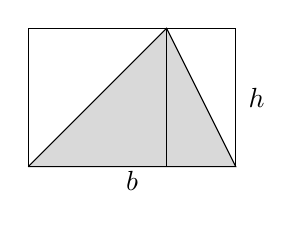
\begin{tikzpicture}[x=5em,y=5em]
\fill[color=gray!30] (0,0)--(1,1)--(1.5,0)--(0,0);
\draw (0,0)--(0,1)--(1.5,1)--(1.5,0);
\draw (0,0)--(1,1)--(1.5,0)--(0,0);
\draw (1,1)--(1,0);
\draw (1,1)--(1,0);
\draw (0.75,-.1) node{$b$};
\draw (1.65,.5) node{$h$};
\end{tikzpicture}
\end{center}
\end{floatingfigure}
\end{latexonly}
Seguramente el alumno recuerde toda una colección de fórmulas para calcular el área de polígonos.
Todas esas fórmulas tienen como punto de partida la definición del área de un rectángulo: \emph{el área de un rectángulo es el producto de sus dimensiones.}
A partir de esta definición, podemos calcular el área de cualquier polígono.
Por ejemplo, en la figura de la izquierda, podemos ver que el área de  un triángulo de base $b$ y altura $h$ es
$A=\frac12bh$ (ya que el área de los dos triángulos sombreados, es igual al área de los dos triángulos sin sombrear).
\begin{rawhtml}
<div class="center">
<img src="./T3/figuras/Leccion33-1.svg" width="150">
</div>
\end{rawhtml}
Además, el área de cualquier otra \emph{región poligonal} se puede calcular dividiéndola en triángulos.
%
\begin{latexonly}
\begin{center}
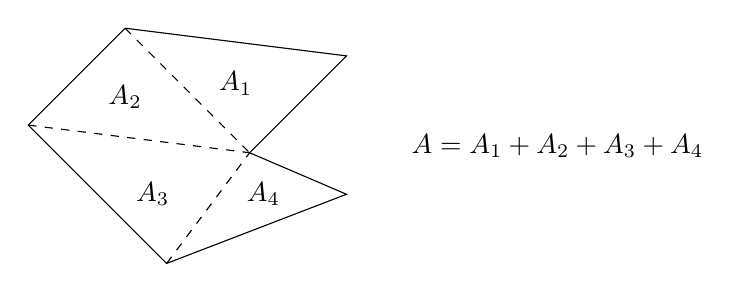
\begin{tikzpicture}[x=5em,y=5em]
\draw (1,0)--(0,1)--(.7,1.7)--(2.3,1.5)--(1.6,.8)--(2.3,.5)--(1,0);
\draw[dashed] (.7,1.7)--(1.6,.8);
\draw[dashed] (0,1)--(1.6,.8);
\draw[dashed] (1,0)--(1.6,.8);
\draw (1.5,1.3) node{$A_1$};
\draw (.7,1.2) node{$A_2$};
\draw (.9,.5) node{$A_3$};
\draw (1.7,.5) node{$A_4$};
\draw (2.7,.85) node[right]{$A=A_1+A_2+A_3+A_4$};
\end{tikzpicture}
\end{center}
\end{latexonly}
\begin{rawhtml}
<p></p>
<div class="center">
<img src="./T3/figuras/Leccion33-2.svg" width="450">
</div>
\end{rawhtml}

Pero, ¿cómo calculamos el área encerrada por una curva?
No podemos obtener de forma directa una expresión para esa área, por lo que, en estos casos, buscamos un procedimiento para aproximar su valor.
Por ejemplo, en la antigüedad, utilizaban polígonos regulares inscritos en un círculo para aproximar el valor de su área; cuantos más lados tomemos, mejor será esta aproximación.

\begin{latexonly}
\begin{center}
\begin{tikzpicture}
\foreach \rr in {3,...,7}{
\draw[gray!70](\rr*2,0) circle (2em);
\node[regular polygon, regular polygon sides=\rr, minimum size=4em, draw]
at (\rr*2,0) {};}
\end{tikzpicture}
\end{center}
\end{latexonly}
\begin{rawhtml}
<div class="center">
<img src="./T3/figuras/Leccion33-3.svg" width="450">
</div>
\end{rawhtml}


En una región arbitraria, también podemos utilizar este procedimiento, por ejemplo, inscribiendo franjas rectangulares para obtener aproximaciones que podemos mejorar tomandolas cada vez más estrechas.

\begin{latexonly}
\begin{center}
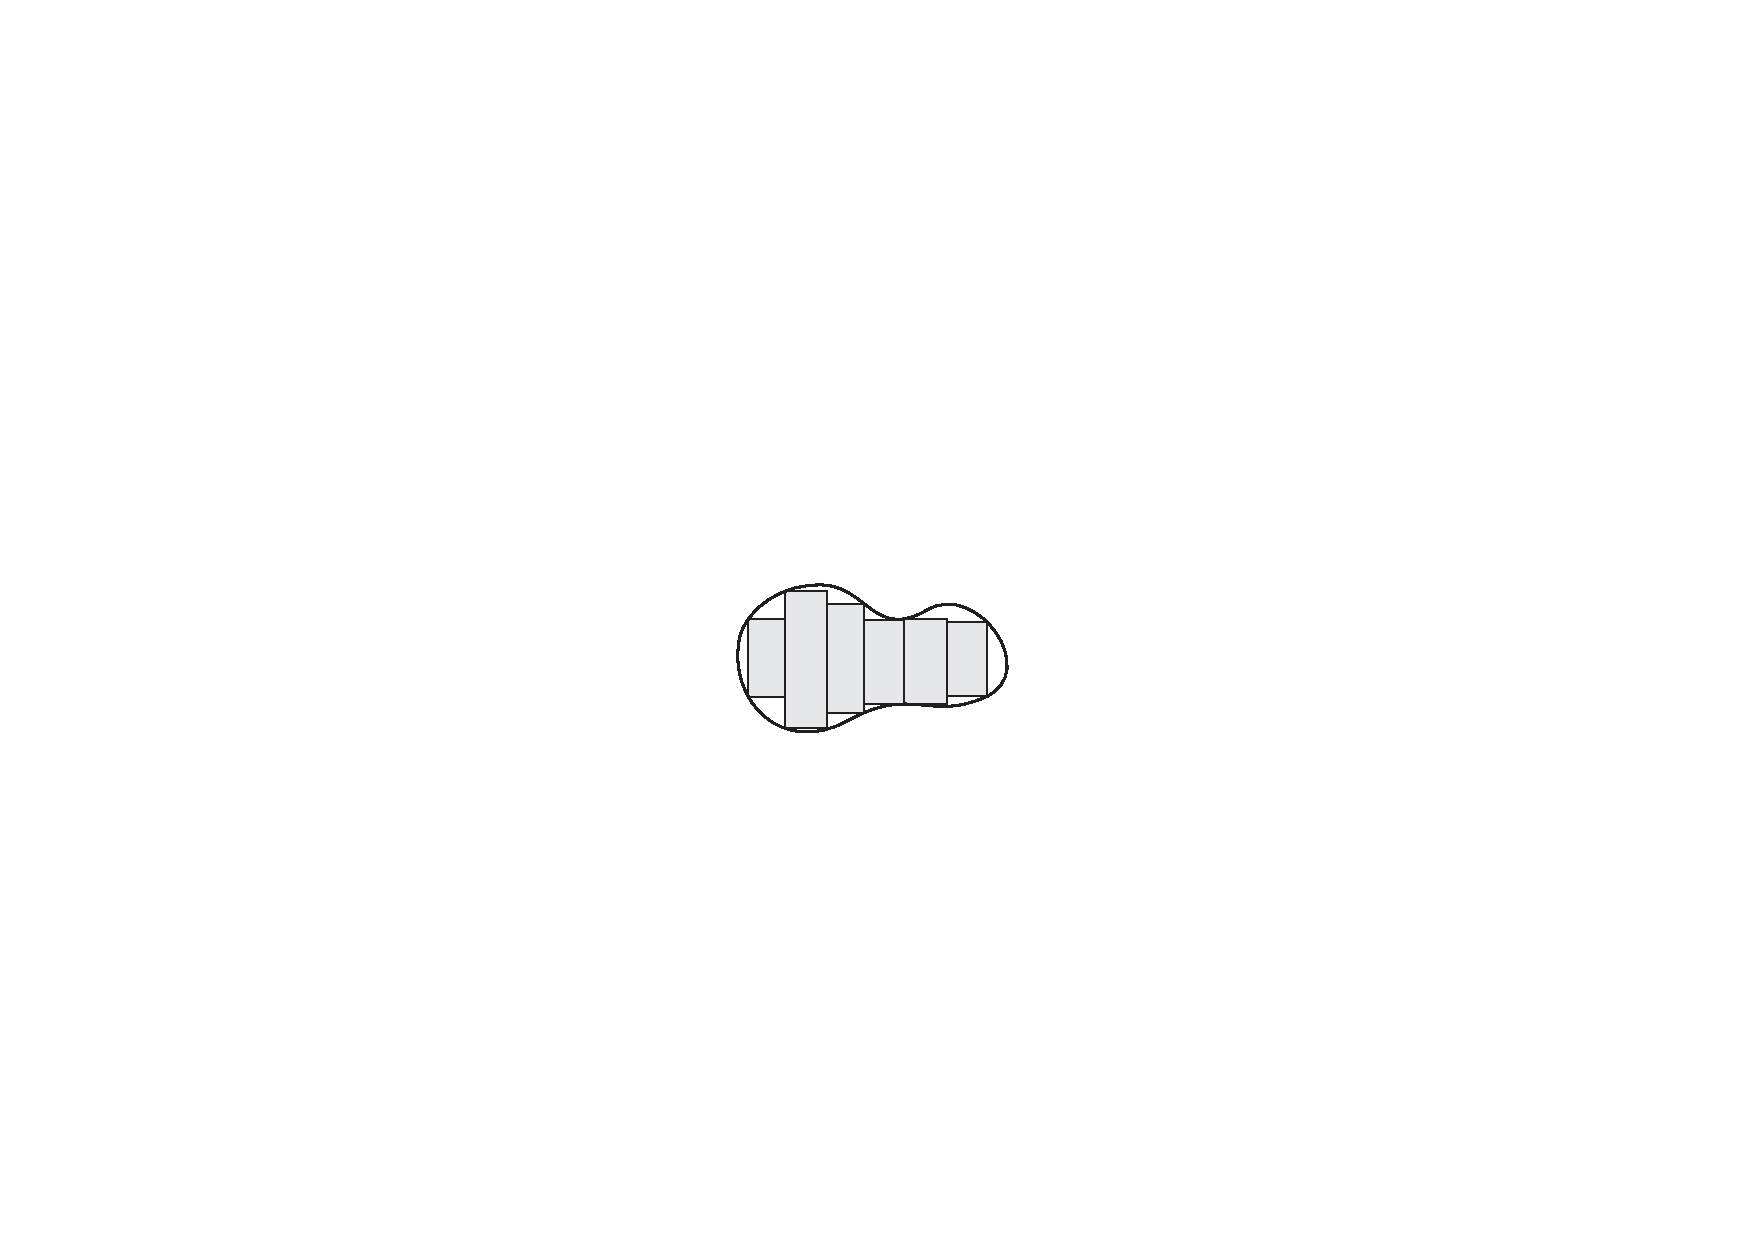
\includegraphics{T3/figs/DefArea2.pdf}
\end{center}
\end{latexonly}
\begin{rawhtml}
<div class="center">
<img src="./T3/figuras/Leccion33-4-DefArea2.svg" width="300">
</div>
\end{rawhtml}
%
De hecho, este es el punto de partida para definir las \emph{sumas de Riemann}, que introducimos a continuación, y que son el fundamento de la \emph{Integral de Riemann}.

\subsection{Sumas de Riemann: integración numérica}

Si $f$ es una función positiva en el intervalo $[a,b]$, queremos calcular el área de la región comprendida entre el grafo de $f$, el eje $OX$ y las rectas $X=a$ y $X=b$.
Este área será la integral definida de $f$ en el intervalo $[a,b]$.
%
\begin{latexonly}
\begin{center}
\begin{tikzpicture}[x=3em,y=3em]
%\pgfsetlinewidth{.5pt}
% Zona sombreada:
% Una vez generada la curva, duplico el archivo .table
% y le añado los puntos que cierran la región.
% De esta forma, puedo utilizar \fill para crear la
% región sobreada:
\fill[gray!30] plot file {T3/figs/Calc3.riemann2.table};
\draw[domain=1:5,smooth,variable=\x]
plot (\x,0.2*\x*\x*\x-1.7*\x*\x+4.0*\x-.5);
%
\draw (1,2.0) -- (1,0) node[below] {$a$};
\draw (5,2)--(5,0) node[below] {$b$};
\draw[latex-] (4,.7)--(6,1.5) node[right]{Área$=\displaystyle\int_a^b f(x)\mathrm dx$};
% Ejes
\draw[-stealth] (-.15,0) -- (5.7,0) node[right] {$X$}; 
\draw[-stealth] (0,-.15) -- (0,2.5) node[right] {$Y$};;
\end{tikzpicture}
\end{center}
\end{latexonly}
\begin{rawhtml}
<div class="center">
<img src="./T3/figuras/Leccion33-5.svg" width="400">
</div>
\end{rawhtml}
%
Con este modelo, podemos plantear fácilmente los cálculos necesarios para aproximar el valor de la integral como la suma de las áreas de varios rectángulos.
Para describir estos rectángulos, elegimos un conjunto de puntos $x_k$, tales que
\[
a=x_0 \sle x_1 \sle x_2 \sle \dots \sle x_{m-1} \sle x_m=b,
\]
y puntos intermedios $s_k$ tales que $x_{k-1}\le s_k\le x_k$, de tal forma que cada subintervalo
$[x_{k-1},x_k]$ será la base de un rectángulo y $f(s_k)$ su altura.
El área de cada rectángulo será $f(s_k)(x_k-x_{k-1})$ y por lo tanto, la aproximación del área de la región será la suma de las áreas de todos estos rectángulos, es decir
\enlargethispage{\baselineskip}
\[
\sum_{k=1}^m f(s_k)(x_k-x_{k-1}).
\]
Esta aproximación corresponde a la región sombreada que podemos ver en la figura~\ref{fig:sum-rie} y la expresión se denomina \emph{Suma de Riemann}.
\begin{rawhtml}
<div class="center">
<img src="./T3/figuras/Leccion33-6.svg" width="400">
</div>
\end{rawhtml}
%
\begin{latexonly}
\begin{figure}
\begin{center}
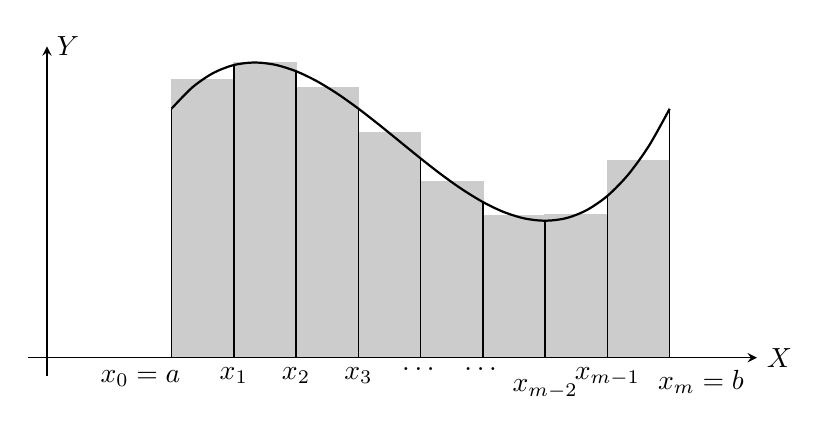
\begin{tikzpicture}[x=4.5em,y=4.5em]
\pgfsetlinewidth{.5pt}
% Zona sombreada (suma de Riemann)
\draw[gray!40,fill=gray!40] (1,0) -- (1,2.234375) -- (1.5,2.234375) -- (1.5,2.365625000000001) -- (2,2.365625000000001) -- (2,2.171875) -- (2.5,2.171875) -- (2.5,1.803125000000001) -- (3,1.803125000000001) -- (3,1.409375000000004) -- (3.5,1.409375000000004) -- (3.5,1.140625) -- (4,1.140625) -- (4,1.146875000000003) -- (4.5,1.146875000000003) -- (4.5,1.578125000000004) -- (5,1.578125000000004) -- (5,0) -- (1,0);
% Ejes y función:
\draw[-stealth] (-.15,0) -- (5.7,0) node[right] {$X$}; 
\draw[-stealth] (0,-.15) -- (0,2.5) node[right] {$Y$};;
\draw[thick,domain=1:5,smooth,variable=\x]
plot (\x,0.2*\x*\x*\x-1.7*\x*\x+4.0*\x-.5);
\draw (.75,-.02) node[below] {$x_0=a$};
\draw (1,2.0) -- (1,0);
\draw (1.5,2.35) -- (1.5,0) node[below] {$x_1$};
\draw (2,2.3)--(2,0)  node[below] {$x_2$};
\draw (2.5,2) -- (2.5,0) node[below] {$x_3$};
\draw (3,1.6) --(3,0) node[below]{\dots};
\draw (3.5,1.25) -- (3.5,0) node[below]{\dots}; 
\draw (4,1.1) -- (4,0);
\draw (4,-.1) node[below]{$x_{m-2}$};
\draw (4.5,1.3) -- (4.5,0) node[below]{$x_{m-1}$};
\draw (5,2)--(5,0);
\draw (5.25,-.02) node[below] {$x_m=b$};
\end{tikzpicture}
\end{center}
\caption{Aproximación del área bajo el grafo usando sumas de Riemann.}\label{fig:sum-rie}
\end{figure}
%
\begin{figure}
\begin{center}
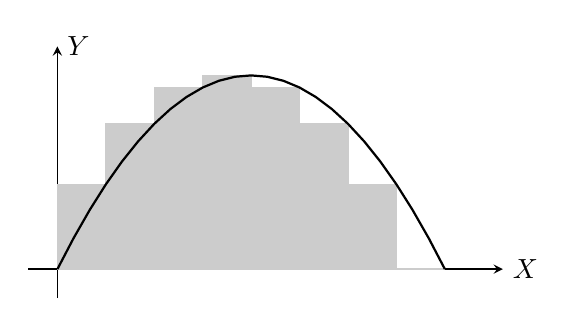
\begin{tikzpicture}[x=7em,y=7em]
\pgfsetlinewidth{.5pt}
\draw[-stealth] (-.15,0) -- (2.3,0) node[right] {$X$}; 
\draw[-stealth] (0,-.15) -- (0,1.15) node[right] {$Y$};;
\draw[gray!40,fill=gray!40](0,0)--(0,0.4375)--(0.25,0.4375)--(0.25,0.75)--(0.5,0.75)--(0.5,0.9375)--(0.75,0.9375)--(.75,1)--(1,1)
--(1,0.9375)--(1.25,0.9375)--(1.25,0.75)--(1.5,0.75)--(1.5,0.4375)--(1.75,0.4375)--(1.75,0)--(2,0)--(0,0);
\draw[thick,domain=0:2] plot (\x,2*\x-\x*\x);
%plot[id=parab8,samples=50]
%function{2*x-x*x};
\end{tikzpicture}
\end{center}
\caption{Aproximación del área del ejemplo~\ref{ej-riemann}.}\label{fig:ej-riemann}
\end{figure}
\end{latexonly}
\begin{ejemplo}\label{ej-riemann}
%
Consideremos la función $f(x)=2x-x^2$ en el intervalo $[0,2]$ y
consideremos los puntos $x_k=\dfrac{k}4$, $s_k=\dfrac{k}4$ para cada $k=0,1,\dots,8$;
con ellos, vamos a calcular una aproximación del área que queda debajo de la gráfica de $f$, según aparece en la figura~\ref{fig:ej-riemann}.
\begin{rawhtml}
<div class="center">
<img src="./T3/figuras/Leccion33-7.svg" width="400">
</div>
\end{rawhtml}
En primer lugar, observamos que, para cada $k=1,\dots,8$
\enlargethispage{-1.2ex}
\[
x_k-x_{k-1} = \frac{k}4 - \frac{k-1}4 = \frac14,
\]
y por lo tanto
\begin{multline*}
\sum_{k=1}^m f(s_k)(x_k-x_{k-1})
= \sum_{k=1}^8 f\big(\frac{k}4\big)\frac14
= \frac14\sum_{k=1}^8 \big(2\frac{k}4-\frac{k^2}{16}\big)=\\
= \frac14\big(\big(\frac{1}2-\frac{1^2}{16}\big) +
 \big(\frac{2}2-\frac{2^2}{16}\big) +
 \big(\frac{3}2-\frac{3^2}{16}\big) +
 \big(\frac{4}2-\frac{4^2}{16}\big) +\\
 +\big(\frac{5}2-\frac{5^2}{16}\big) +
 \big(\frac{6}2-\frac{6^2}{16}\big) +
 \big(\frac{7}2-\frac{7^2}{16}\big) +
 \big(\frac{8}2-\frac{8^2}{16}\big)\big) =\frac{21}{16}\tag*{\fej}
\end{multline*}
\end{ejemplo}

Las aproximaciones dadas por las sumas de Riemann pueden ser mejoradas aumentando el número de puntos, de forma que la amplitud de todos los subintervalos disminuya tendiendo a 0.
Decimos que una función es integrable si, en estas condiciones, las sumas de Riemann convergen a un mismo valor y este valor se denomina \emph{integral (definida)} de la función en el intervalo.

\begin{ejemplo}\label{ej-parab}
Vamos a considerar nuevamente la función $f(x)=2x-x^2$ del ejemplo anterior.
Pero ahora, vamos a calcular las sumas de Riemann para una partición en $n$ subintervalos iguales, es decir, de amplitud $\dfrac2n$, y tomando igualmente el extremo superior como punto intermedio de cada subintervalo;
es decir, $s_{n,k}=x_{n,k} = \dfrac{2k}n$ para $k=1,\dots,n$ y entonces,
\begin{align*}
\sum_{k=1}^n f(s_{n,k})(x_{n,k}-x_{n,k-1})
& = \frac2n\sum_{k=1}^n f(s_{n,k}) = \frac2n\sum_{k=1}^n f(\frac{2k}n)=\\
& = \frac2n \sum_{k=1}^n \big(2\frac{2k}n-\frac{4k^2}{n^2}\big)= \\
& = \left(\left( \frac8{n^2}\sum_{k=1}^n k\right) -\left( \frac8{n^3}\sum_{k=1}^n k^2\right)\right)=\\
& = \left(\left( \frac8{n^2}\frac{n(n+1)}2\right) -\left( \frac8{n^3}\frac{n(n+1)(2n+1)}6\right)
\right)=\\
& =\frac{4n^2-4}{3n^2}
\end{align*}
Entonces,
\[
\int_0^2(2x-x^2)\mathrm dx = \lim \frac{4n^2-4}{3n^2} =\frac43\tag*{\fej}
\]
%Ahora podemos comparar este resultado con la aproximación obtenida en el ejemplo~\ref{ej-riemann}:
%\[
%\text{Error}=\frac43-\frac{21}{16} =\frac1{48} = 0.0208 \wideparen3 
%\]
\end{ejemplo}

%Si la función es positiva en el intervalo, el valor de esta integral es el área de la región que queda entre el grafo y el eje~$OX$.

En particular, las funciones continuas son integrables en cada intervalo cerrado contenido en su dominio y estas funciones serán con las que trabajaremos en el curso.
Para calcular integrales definidas usamos el cálculo de primitivas (si es posible) y usamos las sumas de Riemann como método de aproximación.
No obstante, debemos entender que la teoría asociada a las sumas de Riemann no es solo importante como método de aproximación, sino que además es la forma de probar que una magnitud puede definirse o calcularse mediante integrales: cualquier magnitud que se puede aproximar por sumas de Riemann de una función continua, tiene a la integral como valor exacto; más adelante, veremos algunos ejemplos intuitivos de estas ideas.

\begin{rawhtml}
<p style="text-align: center;"><iframe width="560" height="316" src="https://www.youtube.com/embed/rWzW0uggaN0?list=PL2rtpLKW91qawRYK1FOQv2H_dcdGz_dIo" frameborder="0" allowfullscreen=""></iframe></p>
\end{rawhtml}


\subsection{Regla de Barrow y propiedades}

Ya hemos recordado en la primera lección de este tema el teorema fundamental de cálculo, que establece que si $f$ es continua, la función
\[
F(x)=\int_a^x f(t)\mathrm dt,
\]
es una primitiva de $f$, es decir, $F'(x)=f(x)$.
A partir de este teorema se deduce fácilmente la Regla de Barrow, que es la herramienta para cálculo de integrales basada en primitivas.
Supongamos que $G$ es cualquier primitiva de $f$, que habremos hallado usando los métodos vistos en la primera lección de este tema.
Entonces $F$ y $G$ se diferencian en una constante,
\begin{equation}\label{eq:barrow1}
G(x)-\int_a^x f(t)\mathrm dt = C, \text{ para todo } x\in[a,b]
\end{equation}
En particular, tomando $x=a$ determinamos el valor de $C$:
\[
C=G(a)-\int_a^a f(t)\mathrm dt = G(a)
\]
y con él, ya podemos expresar el valor de la integral definida en terminos de $G$:
\[
\int_a^x f(t)\mathrm dt = G(x)-G(a).
\]
De esta forma, hemos demostrado la regla de Barrow.
%
\begin{teorema}[Regla de Barrow]\label{th:barrow}
Si $f$ es continua en $[a,b]$ y $G'(x)=f(x)$ para todo $x\in[a,b]$, entonces 
\[ 
\int_a^b f(t)\,\mathrm dt=G(b)-G(a) \stackrel{\text{(Notación)}}{=} \left[G(x)\vphantom{\dfrac12}\right]_a^b
\]
\end{teorema}
\begin{rawhtml}
&nbsp;
\end{rawhtml}
\begin{ejemplo}
Vamos a calcular de nuevo el área de la región del ejemplo~\ref{ej-parab} usando la regla de Barrow:
\begin{equation}
\int_0^2 (2x-x^2)\mathrm dx = \left[x^2-\frac{x^3}3\right]_0^2 = 4-\frac83=\frac43\tag*{\fej}
\end{equation}
\end{ejemplo}
\begin{rawhtml}
&nbsp;
\end{rawhtml}
\begin{ejemplo}\label{ej-circ}
El área de un círculo se puede calcular a partir de la gráfica de la función $f(x)=\sqrt{r^2-x^2}$. Si consideremos el intervalo $[0,r]$, la región entre el grafo de $f$ y el eje $OX$ es un cuarto de círculo y por lo tanto:
\[
A=4\int_0^r\sqrt{r^2-x^2}\mathrm dx
\]
Hallamos en primer lugar la primitiva:
\begin{align*}
A =& 4\int \sqrt{r^2-x^2}\mathrm dx=\\
&\left[
\begin{array}{l}
x=r\operatorname{sen}\theta %\text{ (esta función es creciente en $[0,\pi/2]$)}\\
\mathrm dx=r\cos\theta d\theta
\end{array}
\right.\\
=& 4\int \sqrt{r^2-r^2\operatorname{sen}^2\theta}\, r\cos\theta\, d\theta=\\
= & 4\int r^2\cos^2\theta d\theta
= 4r^2\int \left(\frac12+\frac12\cos2\theta\right) d\theta=\\
= & 4r^2\left(\frac{\theta}2+\frac14\operatorname{sen} 2\theta\right)
= r^2\left(2\theta +\operatorname{sen} 2\theta\right)=\\
= & r^2\Big(2\operatorname{arcsen}\frac{x}{r} +\operatorname{sen} 2(\operatorname{arcsen}\frac{x}{r})\Big)
\end{align*}
Por lo tanto
\begin{multline*}
A=4\int_0^r\sqrt{r^2-x^2}\mathrm dx=
\left[r^2\Big(2\operatorname{arcsen}\frac{x}{r} +\operatorname{sen} 2(\operatorname{arcsen}\frac{x}{r})\Big)\right]_0^r=\\
=r^2\Big(2\operatorname{arcsen} 1 +\operatorname{sen} 2(\operatorname{arcsen} 1)\Big)
-r^2\Big(2\operatorname{arcsen} 0 +\operatorname{sen} 2(\operatorname{arcsen} 0)\Big)=\\
=r^2\Big(2\frac{\pi}2 +\operatorname{sen} 2(\frac{\pi}2)\Big)
=\pi r^2\tag*{\fej}
%\left[2r^2\operatorname{arcsen}\dfrac{x}r +2x\sqrt{r^2-x^2}\right]_0^r=\pi r^2
\end{multline*}
\end{ejemplo}

Debemos insistir en que el hecho de tener un resultado tan potente como la Regla de Barrow para calcular integrales definidas, no debe llevarnos a la conclusión errónea de que podemos olvidar la definición de integral.
De hecho, la regla de Barrow solo es útil para aquellas funciones que admiten una primitiva \emph{expresable en términos de funciones elementales}, y ya sabemos que no todas las funciones continuas admiten este tipo de primitivas.

\begin{teorema}[Linealidad de la integral]
Si $f$ y $g$ son continuas en $[a,b]$ y $\alpha,\beta\in\mathbb{R}$, entonces:
\[
\int_a^b(\alpha f(x)+\beta g(x))\,\mathrm dx=
\alpha\int_a^b f(x)\,\mathrm dx +\beta \int_a^b g(x)\,\mathrm dx
\]
\end{teorema}
\begin{rawhtml}
&nbsp;
\end{rawhtml}
\begin{teorema}[Propiedad de aditividad] Sea $f$ una función continua en $[a,b]$ y
$c\in[a,b]$, entonces
\[
\int_a^b f(x)\,\mathrm dx =\left(\int_a^c f(x)\,\mathrm dx\right)+
\left(\int_c^b f(x)\,\mathrm dx\right)
\]
\end{teorema}
%
Tal y como hemos definido la integral, en el operador $\displaystyle\int_a^b$ es necesario que $a\le b$.
Para flexibilizar los cálculos, es conveniente admitir la situación inversa.
%
\begin{definicion}
Si $f$ es continua en $[a,b]$, definimos la integral
$\displaystyle\int_b^af(x)\,\mathrm dx$ como:
\[
\int_b^a f(x)\,\mathrm dx = -\int_a^b f(x)\,\mathrm dx
\]
\end{definicion}

Esta definición se hace así para que la extensión del operador siga verificando la propiedad de aditividad
\begin{align*}
& \int_a^bf(x)\,\mathrm dx+\int_b^af(x)\,\mathrm dx = \int_a^a f(x)\,\mathrm dx =0\\
& \int_a^bf(x)\,\mathrm dx+\int_b^af(x)\,\mathrm dx = \int_a^bf(x)\,\mathrm dx-\int_a^bf(x)\,\mathrm dx = 0
\end{align*}

A continuación, vamos a dar los enunciados de los teoremas de cambio de variable e integración por partes, pero para integrales definidas.
Si utilizamos estos métodos para calcular integrales definidas, es preferible usarlos tal y como los enunciamos a continuación ya que, como veremos en los ejemplos, su aplicación simplifica los cálculos necesarios.
%
\begin{teorema}[Cambio de variable directo]\label{th:sust1}
Supongamos que $g'$ es continua y en $[a,b]$ y que $f$ es continua y biyectiva entre $g(a)$ y $g(b)$,
entonces:  
\[
\int_a^bf(g(x))g'(x)\mathrm dx = \int_{g(a)}^{g(b)}f(u)\mathrm du
\]
\end{teorema}
\begin{rawhtml}
&nbsp;
\end{rawhtml}
\begin{corolario}[Cambio de variable inverso]\label{th:sust2}
Sea $f$ una función continua en $[\alpha ,\beta]$.
Consideremos una función $g\colon I\to [\alpha ,\beta]$ biyectiva, continua y con primera derivada continua. Entonces, 
\[
\int_\alpha^\beta f(x)\mathrm dx = 
\int_{g^{-1}(\alpha)}^{g^{-1}(\beta)}f(g(u))g'(u)\mathrm du
\]
\end{corolario}

Obsérvese que, en este teorema, hemos incluido, como condición necesaria, que el cambio de variable esté dado por una función biyectiva, es decir, monótona en el intervalo de integración.
%
\begin{ejemplo}
Vamos a repetir el cálculo del área de un círculo de radio $r$, que hicimos anteriormente, pero de forma más simple por la ayuda del resultado anterior:
\begin{align*}
A =& 4\int_0^r\sqrt{r^2-x^2}\mathrm dx=\\
&\left[
\begin{array}{l}
x=r\operatorname{sen}\theta \text{ (esta función es creciente en $[0,\pi/2]$)}\\
\mathrm dx=r\cos\theta d\theta\\
x_0=0 \Rightarrow \theta_0=\operatorname{arcsen} 0 = 0\\
x_1=r \Rightarrow \theta_1=\operatorname{arcsen}\frac{r}r =\operatorname{arcsen}1 = \pi/2\\
\end{array}
\right.\\
= & 4\int_0^{\pi/2}r^2\cos^2\theta d\theta
= 4r^2\int_0^{\pi/2}\left(\frac12+\frac12\cos2\theta\right) d\theta=\\
= & 4r^2\left[\frac{\theta}2+\frac14\operatorname{sen} 2\theta\right]_0^{\pi/2}
= 4r^2 \dfrac{\pi}4 = \pi r^2\tag*{\fej}
\end{align*}
\end{ejemplo}
\begin{rawhtml}
&nbsp;
\end{rawhtml}
\begin{teorema}[Integración por partes]\label{th:partes}
Sean $f$ y $g$ dos funciones tales que $f'$ y $g'$ son  continuas, entonces:
\[
\int_a^bf(x)g'(x)\mathrm dx = \left[f(x)g(x)\vphantom{\frac12}\right]_a^b-\int_a^bg(x)f'(x)\mathrm dx
\]
\end{teorema}
\begin{rawhtml}
&nbsp;
\end{rawhtml}
\begin{ejemplo}
Utilizamos el resultado anterior para calcular la siguiente integral definida
\[
\int_{\pi/6}^{\pi/2}\cos x \log\operatorname{sen} x\,\mathrm dx
\]
Para ello, utilizamos el cambio de variable
\[
t = \operatorname{sen} x,\quad
\mathrm dt = \cos x\,\mathrm dx
\]
Los límites de integración se modifican de la siguiente forma: para $x=\pi/6$, el valor de $t$ es  $1/2$, mientras que para $x=\pi/2$ el valor de $t$ es 1.
%
\begin{align*}
\int_{\pi/6}^{\pi/2}\cos x & \log\operatorname{sen} x\,\mathrm dx =\int_{1/2}^{1} \log t\,\mathrm dt \\
& \left[
\begin{array}{l}
u= \log t \Longrightarrow \mathrm du=\dfrac{\mathrm dt}t \\
\mathrm dv =\mathrm dt \Longrightarrow v=t
\end{array}
\right.\\
= & \left[t\log t\vphantom{\dfrac12}\right]_{1/2}^{1} - \int_{1/2}^{1}\mathrm dt 
= \dfrac{-\log(1/2)}2-\left[t\vphantom{\dfrac12}\right]_{1/2}^{1} = \dfrac{\log 2}2-\dfrac12
\end{align*}
\end{ejemplo}

\begin{rawhtml}
<p style="text-align: center;"><iframe width="560" height="316" src="https://www.youtube.com/embed/aWZcsLIVAAM?list=PL2rtpLKW91qawRYK1FOQv2H_dcdGz_dIo" frameborder="0" allowfullscreen=""></iframe></p>
\end{rawhtml}


\subsection{Aplicaciones geométricas}\label{sec:geom}

Aunque hemos utilizado el cálculo de áreas de regiones planas para motivar el concepto de integral, debemos tener en cuenta que una integral se identifica con un área solo si el integrando es una función positiva.
%
\begin{teorema}
Si $f$ es una función continua y positiva en el intervalo
$[a,b]$, entonces la integral definida $\displaystyle\int_a^b f$ es el valor del área de la región comprendida entre el grafo de $f$ y el eje $OX$ en dicho intervalo.
\end{teorema}

A continuación, repasamos otras aplicaciones de la integral para determinar otras magnitudes, como volúmenes, longitudes de curvas o áreas de superficies alabeadas.
Otras aplicaciones posibles se encuentran en el campo de la física, para calcular el trabajo o los centros de masas.

\paragraph{Cálculo de volúmenes por secciones.}
Supongamos que tenemos el sólido acotado
por dos planos perpendiculares a una recta y que para cada $t\in[a,b]$ conocemos el área $A(t)$, de las secciones del sólido perpendiculares a dicha recta, de tal forma que la función $A$ es continua.
Si tomamos una partición del intervalo, $a=t_0\sle t_1\sle \dots\sle t_n=b$, el volumen del sólido se puede aproximar por la suma de los volúmenes de los cilindros de base $A(t_i)$ y altura $(t_i-t_{i-1})$:
\[
V\approx \sum_{i=1}^n A(t_i)(t_i-t_{i-1})
\]
Obviamente, estas expresiones son sumas de Riemann asociadas a la función $A(t)$, y por lo tanto, podemos afirmar que el volumen exacto es:
\[
V=\int_a^b A(t)\mathrm dt
\]
En algunos casos, el enunciado del problema dará la posición del sólido
respecto de los ejes coordenados, pero más frecuentemente, tendremos que elegir
nosotros esta posición, de tal forma que sea fácil calcular las áreas
$A(t)$.

\begin{ejemplo}\label{ej-cunna}
Se corta una cuña de un tronco (cilíndrico) de radio 2 dm
dando dos cortes con una sierra mecánica que llegan hasta el centro del
tronco. Si uno de los cortes se hace perpendicular y el otro formando un ángulo de
$30^\circ$ con  el primero, ¿qué volumen tendrá la cuña?
\begin{latexonly}
\begin{center}
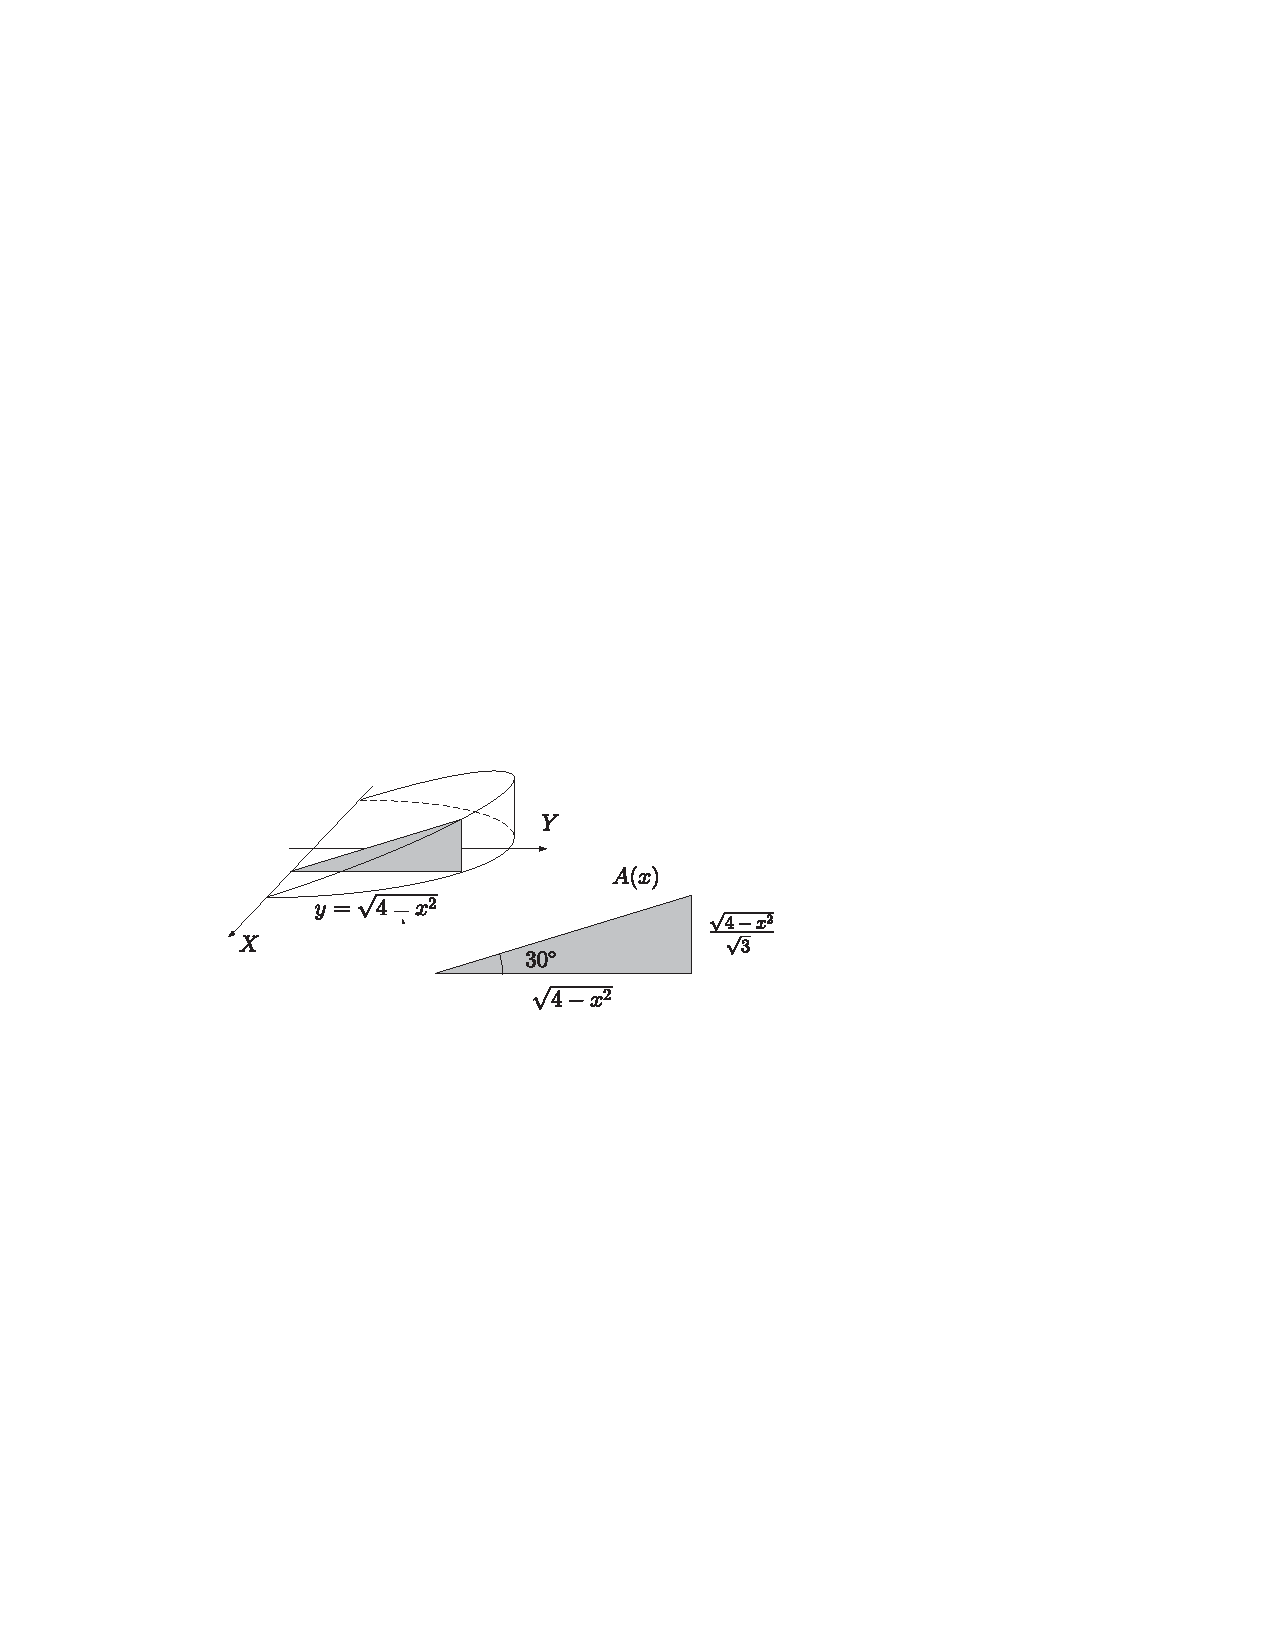
\includegraphics{T3/figs/cunna.pdf}
\end{center}
\end{latexonly}
\begin{rawhtml}
<div class="center">
<img src="./T3/figuras/Leccion33-8-cunna.svg" width="500">
</div>
\end{rawhtml}
Para hacer el cálculo utilizando el método de las secciones, situamos el sólido como se muestra en la figura. La base de la cuña, perpendicular al eje del tronco, es el interior del semicírculo $y=\sqrt{4-x^2}$.
Al hacer los cortes perpendiculares al eje $OX$, las secciones son triángulos rectángulos cuya base es $\sqrt{4-x^2}$ y forma un ángulo de $30^\circ$ con la hipotenusa.
Por lo tanto, su altura es $\frac{\sqrt{4-x^2}}{\sqrt3}$ y el área de la sección es 
$A(x)=\frac1{2\sqrt3}(4-x^2)$. El volumen que queríamos calcular es:
\begin{equation}
V=\int_{-2}^2 A=\int_{-2}^2 \frac{4-x^2}{2\sqrt3}\mathrm dx
=\dfrac{\sqrt3}6 \left[4x-\dfrac{x^3}3\right]_{-2}^2 = \dfrac{16}9\sqrt3
\tag*{\fej}
\end{equation}
\end{ejemplo}

%:Arreglar: expresarlo de una forma más general
% \pi(R(t)^2-r(t)^2)

Como caso particular, podemos calcular el volumen de \emph{sólidos de revolución} usando el método de los discos.
Si consideremos una región plana determinada por el grafo de una función
continua $f$ entre $a$ y $b$ que gira alrededor del eje $OX$,
el sólido generado verifica que las secciones perpendiculares al
eje $OX$, son circulos de radio $f(x)$. Por tanto, el volumen del sólido es:
\[
V=\int_a^b \pi f(x)^2\,\mathrm dx
\]

\paragraph{Cálculo de volúmenes de revolución por capas.}
Otra forma de generar un sólido de revolución es girando la región determinada por una función continua en un intervalo $[a,b]$ con $a\geq 0$, alrededor del eje $OY$. Para aproximar el valor de este volumen, consideremos una partición $a=x_0\sle x_1\sle \dots\sle x_n=b$, y los puntos intermedios $s_i=\frac{x_i+x_{i-1}}2$;
el volumen del sólido se puede aproximar por la suma de los volúmenes de los cilindros cuya base es la corona circular de radios $x_{i-1}$ y $x_i$ y cuya altura es $f(x_i)$:
\begin{multline*}
V \approx \sum_{i=1}^n f(s_i)(\pi x_i^2-\pi x_{i-1}^2) =
\sum_{i=1}^n \pi f(s_i) (x_i+x_{i-i})(x_i-x_{i-i}) = \\ =
\sum_{i=1}^n 2 \pi f(s_i) s_i (x_i-x_{i-i})
\end{multline*}
%
Obviamente, estas expresiones son sumas de Riemann asociadas a la función $2\pi xf(x)$, que es continua por serlo $f$.
Por lo tanto, podemos afirmar que el volumen exacto es
\[
V=\int_a^b 2\pi xf(x)\,\mathrm dx
\]
%
%El método de las secciones es adecuado para sólidos que no presentan \emph{perforaciones}, en estos casos será más recomendable utilizar el método de las capas.

%Para calcular un volumen utilizando cualquiera de los dos métodos, tendremos que situar la región (desplazándola o girándola) en los ejes de coordenadas de tal forma que el cálculo de las secciones o de las capas sea lo más simple posible.

%:Arreglar: expresarlo de una forma más general
% 2\pi*R(t)*h(t), en donde R(t) es el radio de la capa, o distancia al eje,
% y h(t) es la altura de la capa

\paragraph{Longitud de una curva parametrizada.} Si $\gamma(t)=(x(t),y(t))$ es una curva parametrizada diferenciable tal que $x'$ e $y'$ son continuas en $[a,b]$, su longitud viene dada por la siguiente integral:
\[
\ell=\int_a^b\sqrt{(x'(t))^2+(y'(t))^2}\,\mathrm dt
\]
En particular, la \emph{longitud del grafo de una función} $f$, en un intervalo $[a,b]$ es:
\[
L=\int_a^b \sqrt{1+[f'(x)]^2}\,\mathrm dx
\]

\newpage
\thispagestyle{empty}

\ 

\vfill
%\begin{center}
%(Esta página se ha dejado intencionalmente en blanco)
%\end{center}
\newpage


\section{Integración doble} %múltiple

%:Arreglar: Añadir ejemplos de integración doble, prácticamente no hay.

Consideremos un campo escalar $f\colon R\subset\mathbb{R}^2\to \mathbb{R}$ y supongamos que $f$ es positiva
y acotada en el \emph{rectángulo} $R=[a,b]\times[c,d]$. De la misma forma que para las funciones de una variable utilizábamos rectángulos, ahora podemos intentar aproximar el volumen de la región que queda entre el grafo de $f$ y el plano $XY$ tomando prismas.
La manera más simple de hacerlo es tomando particiones de los intervalos $[a,b]$ y $[c,d]$ y considerando, como base de los prismas, los rectángulos que forman:
\begin{latexonly}
\begin{center}
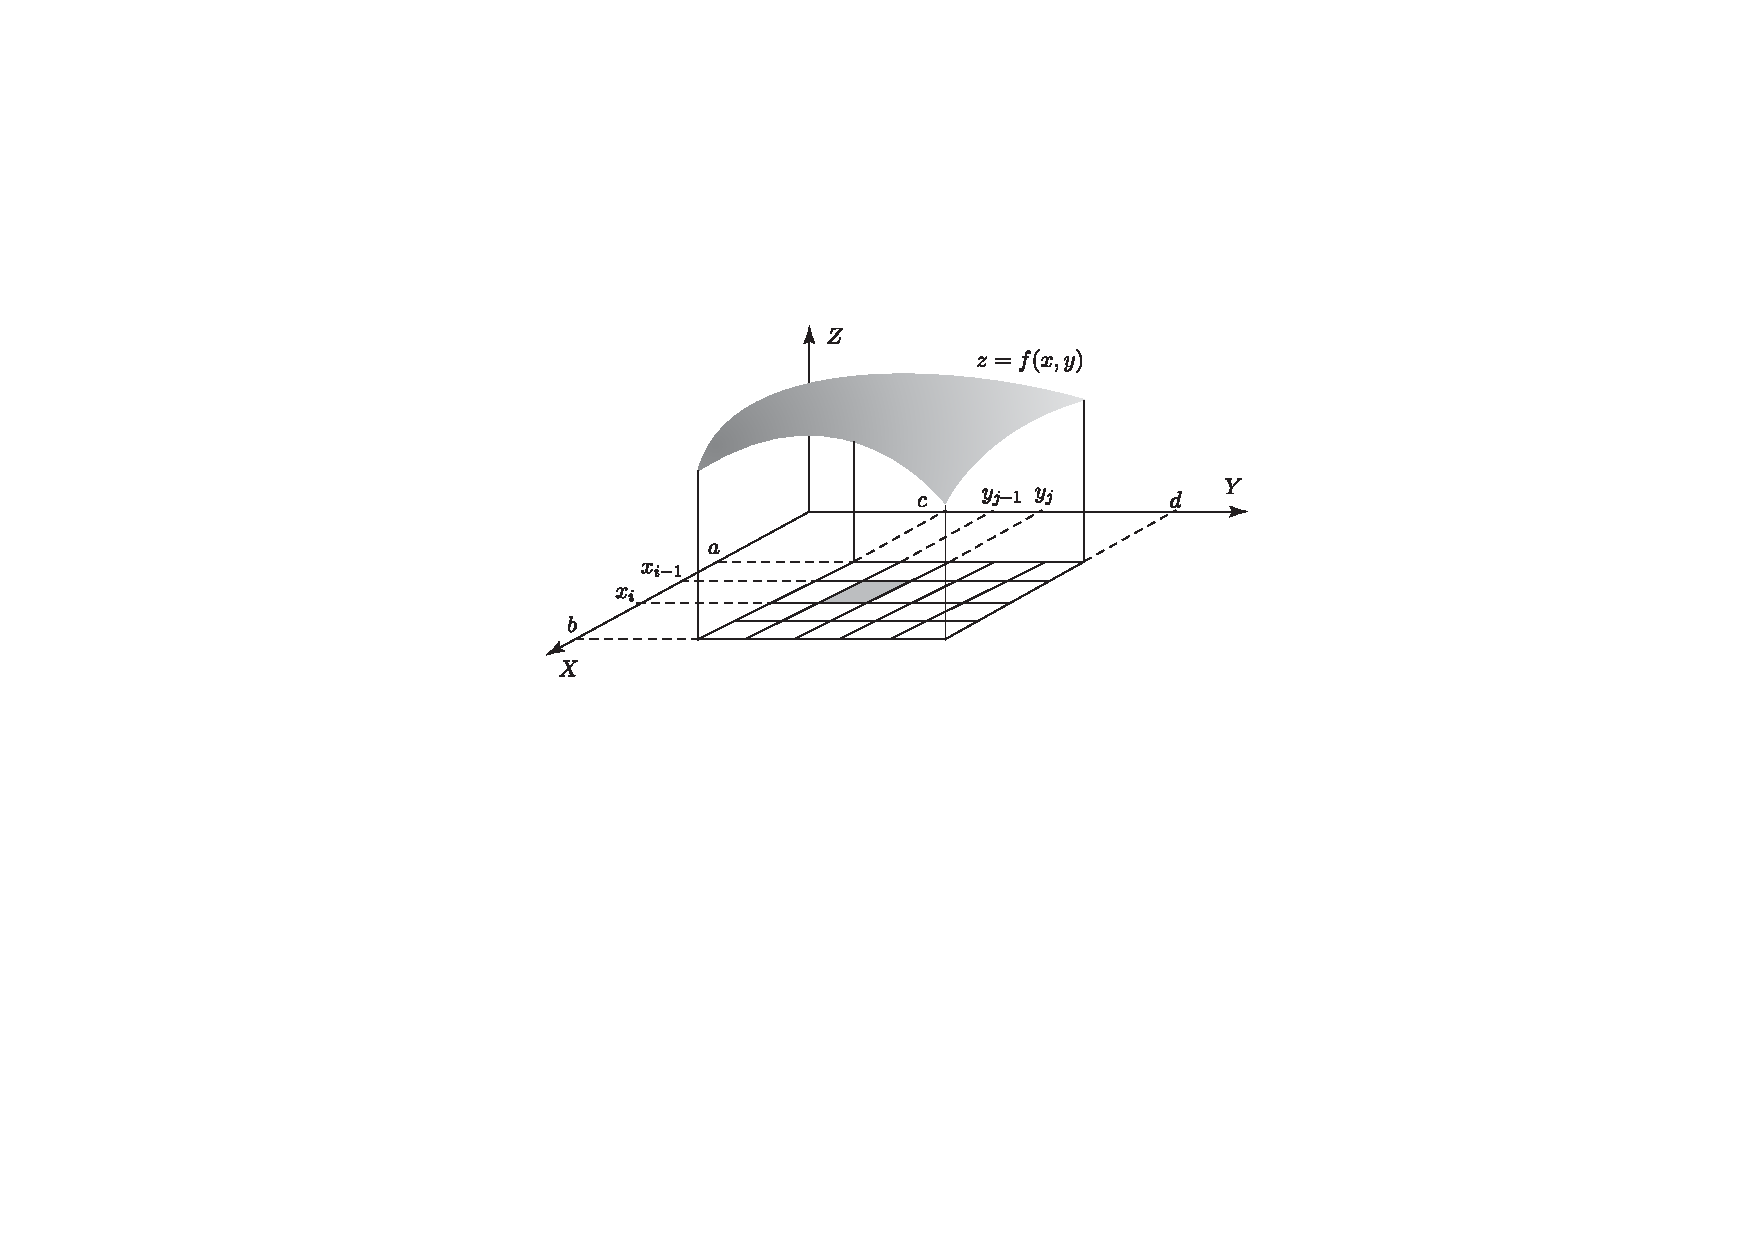
\includegraphics[scale=.8]{T3/figs/IntDoble1.pdf}\\
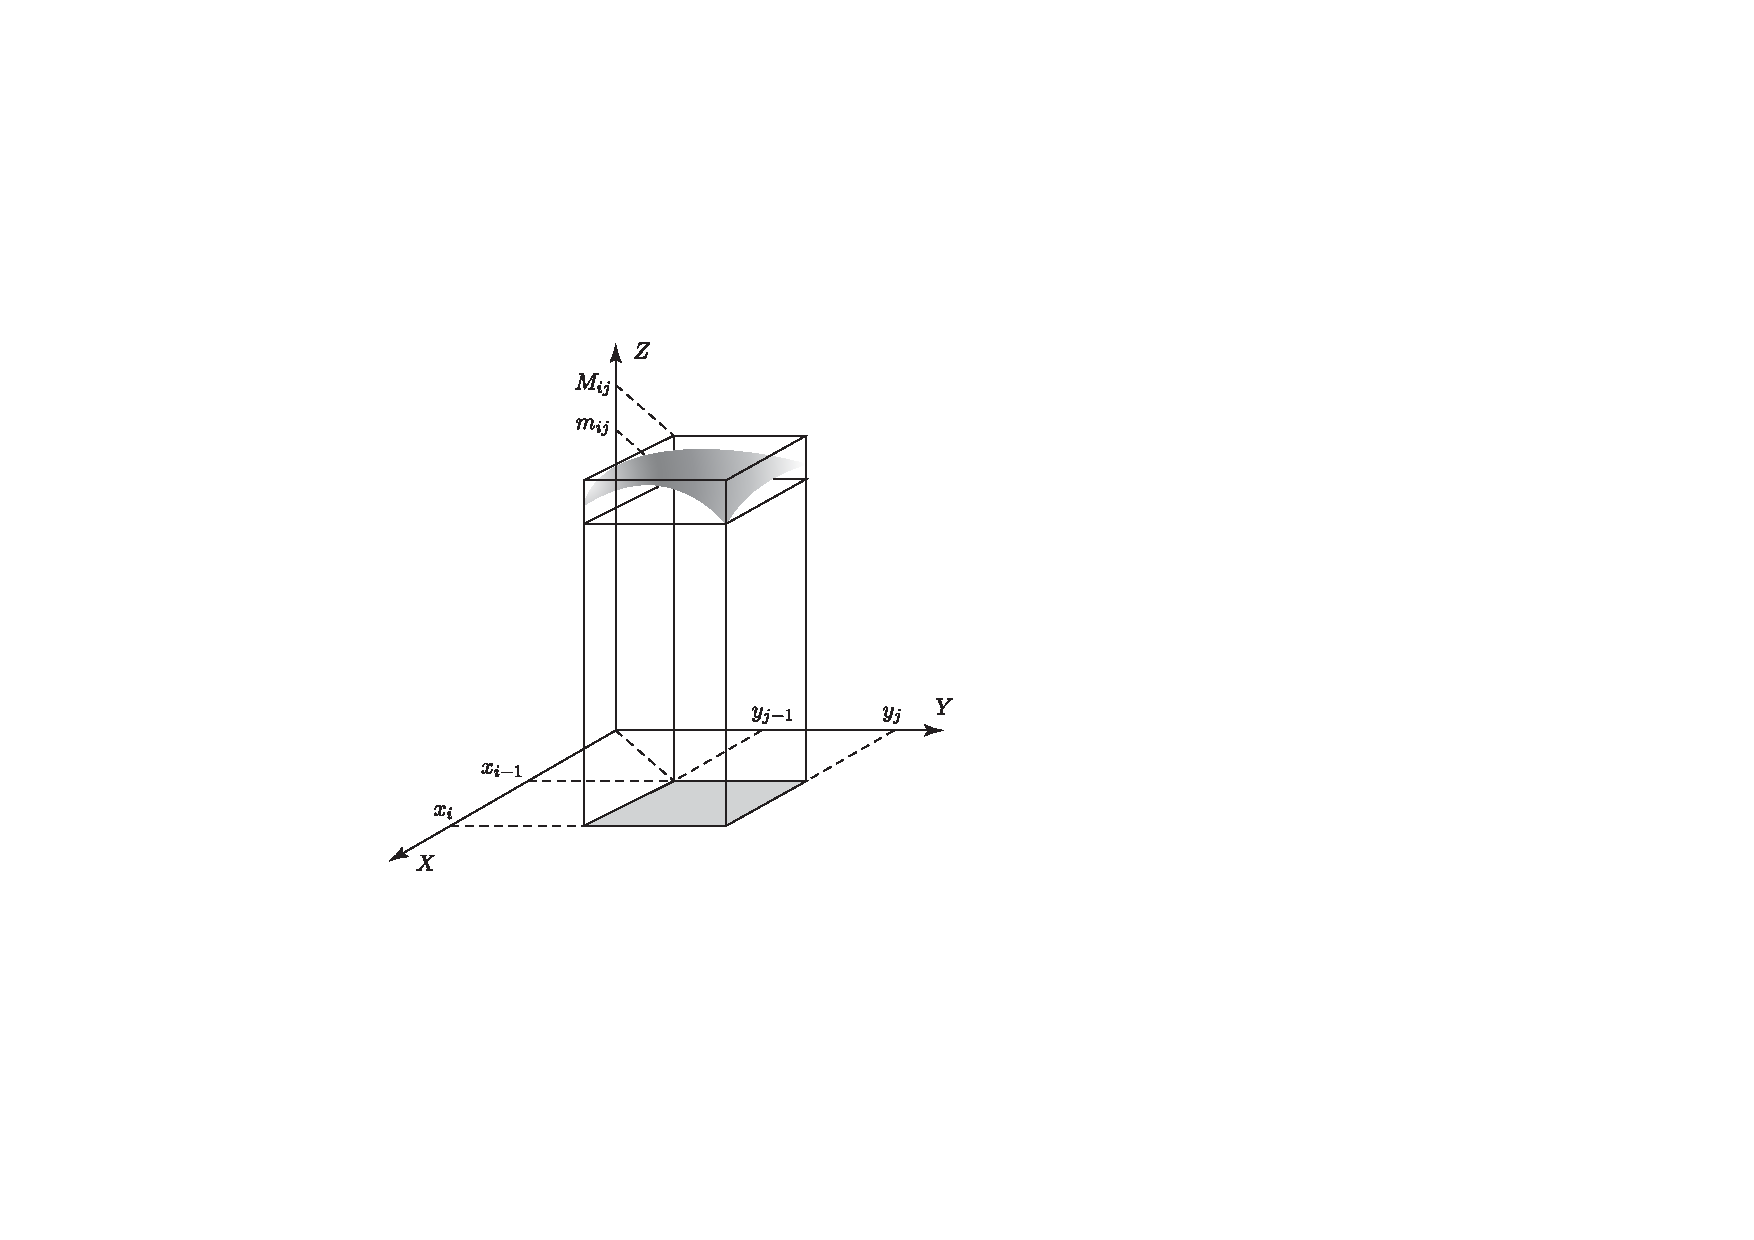
\includegraphics[scale=.8]{T3/figs/IntDoble2.pdf}
\end{center}
\end{latexonly}
\begin{rawhtml}
<div class="center">
<img src="./T3/figuras/Leccion34-1-IntDoble1.svg" width="400">
</div>
<div class="center">
<img src="./T3/figuras/Leccion34-2-IntDoble2.svg" width="400">
</div>
\end{rawhtml}

Podemos tomar aproximaciones por defecto o por exceso considerando los valores máximo y mínimo en el rectángulo como altura del prisma, o tomar una suma de Riemann usando como altura el valor de la función evaluando en cualquier punto interior.
\[
\sum_{i=1}^n\sum_{j=1}^m f(t_i,s_j)(x_i-x_{i-1})(y_j-y_{j-1}),
\]
Como para las funciones de una variable, para mejorar estas aproximaciones basta con tomar más puntos en las particiones, de forma que las áreas de los rectángulos
$R_{ij}=[x_{i-1},x_i]\times[y_{j-1},y_j]$ disminuyan tendiendo a 0.
Diremos que el campo es integrable si, en estas condiciones, las sumas de Riemann convergen a un mismo valor, que denominamos integral de $f$ en la región $R=[a,b]\times[c,d]$:
\[
\iint_Rf(x,y)\mathrm dx\mathrm dy = \lim_{\mathrm{\acute{A}rea}(R_{ij})\to 0} \sum_{i=1}^n\sum_{j=1}^m f(t_i,s_j)(x_i-x_{i-1})(y_j-y_{j-1})
\]
Si el campo es positivo en la región, esta integral es el volumen de la región que queda entre el grafo y el plano $XY$.
En este curso, solo vamos a trabajar con campos continuos, que en particular son integrables, en cualquier región contenida en su dominio.
%
%\begin{ejemplo}
%Vamos a calcular la integral del campo $f(x,y)=2x+y$ en la región $R=[0,1]\times[0,1]$ utilizando particiones regulares de $[0,1]$ en $n$ subintervalos en cada coordenada, y tomando como puntos intermedios los vértices superiores derechos de cada rectángulo.
%\begin{align*}
%\sum_{i=1}^n\sum_{j=1}^n \Big(2\frac{i}{n}+\frac{j}{n}\Big)&\frac{1}{n}\cdot\frac{1}{n}
% =\frac{1}{n^3}\sum_{i=1}^n\sum_{j=1}^n (2i+j)= \frac{1}{n^3}\sum^n_{j=1}\sum^n_{i=1} (2i+j)=\\
%& =\frac{2}{n^3}\Big(\sum^n_{j=1}\sum^n_{i=1} i \Big)
%+\frac{1}{n^3} \Big(\sum^n_{i=1}\sum^n_{j=1} j \Big)=\\
%& =\frac{2}{n^3}\Big(n\cdot\sum^n_{i=1} i \Big)
%+\frac{1}{n^3} \Big(n\cdot \sum^n_{j=1} j \Big)=\\
%& =\frac{2}{n^2}\Big(\sum_{i=1}^n i\Big)
%+\frac{1}{n^2}\Big(\sum_{j=1}^n j\Big)= \\
%& = \frac{3}{n^2}\sum_{i=1}^n i =\frac{3n(n+1)}{2n^2}=\frac{3(n+1)}{2n}
%\end{align*}
%Por lo tanto,
%$\displaystyle\int\limits_R (2x+y)\mathrm dx\mathrm dy = \lim \frac{3(n+1)}{2n}=
%\dfrac{3}{2}$\fej
%\end{ejemplo}

No vamos a abordar en este curso las integrales de campos de tres o más variables, aunque teóricamente su definición no supone ninguna dificultad.
Como veremos a lo largo del tema, el calculo de las integrales múltiples se sustenta en el cálculo de primitivas y en el estudio y transformación de las regiones de integración y por lo tanto, el nivel de dificultad que aporta el aumento de las variables no está en el propio concepto de integral sino en la manipulación de regiones y objetos en el espacio.

\begin{rawhtml}
<p style="text-align: center;"><iframe width="560" height="316" src="https://www.youtube.com/embed/eveq08rsopI?list=PL2rtpLKW91qawRYK1FOQv2H_dcdGz_dIo" frameborder="0" allowfullscreen=""></iframe></p>
\end{rawhtml}

\subsection{Teorema de Fubini. Consecuencias}\label{ejs-fubini}

La definición de integral que hemos dado más arriba establece la forma de saber qué magnitudes pueden se calculadas con la integral de una función, pero no igual que ocurre en funciones de una variable, no constituye un método efectivo de cálculo.
El teorema de Fubini, que enunciamos a continuación, establece la relación entre integrales dobles e integrales de una variable, por lo que, usando conjuntamente con la regla de Barrow, nos da un método de cálculo de integrales basado en el cálculo de primitivas.

\begin{latexonly}
\begin{figure}[p]
\begin{center}
\includegraphics[width=.8\textwidth]{T3/figs/FubIntroX.pdf}\\
$\displaystyle\iint\limits_R f(x,y) = V = \int_a^b A(x)\mathrm dx = \int_a^b \left(\int_c^d f(x,y)\mathrm dy\right)\mathrm dx$\\[6em]
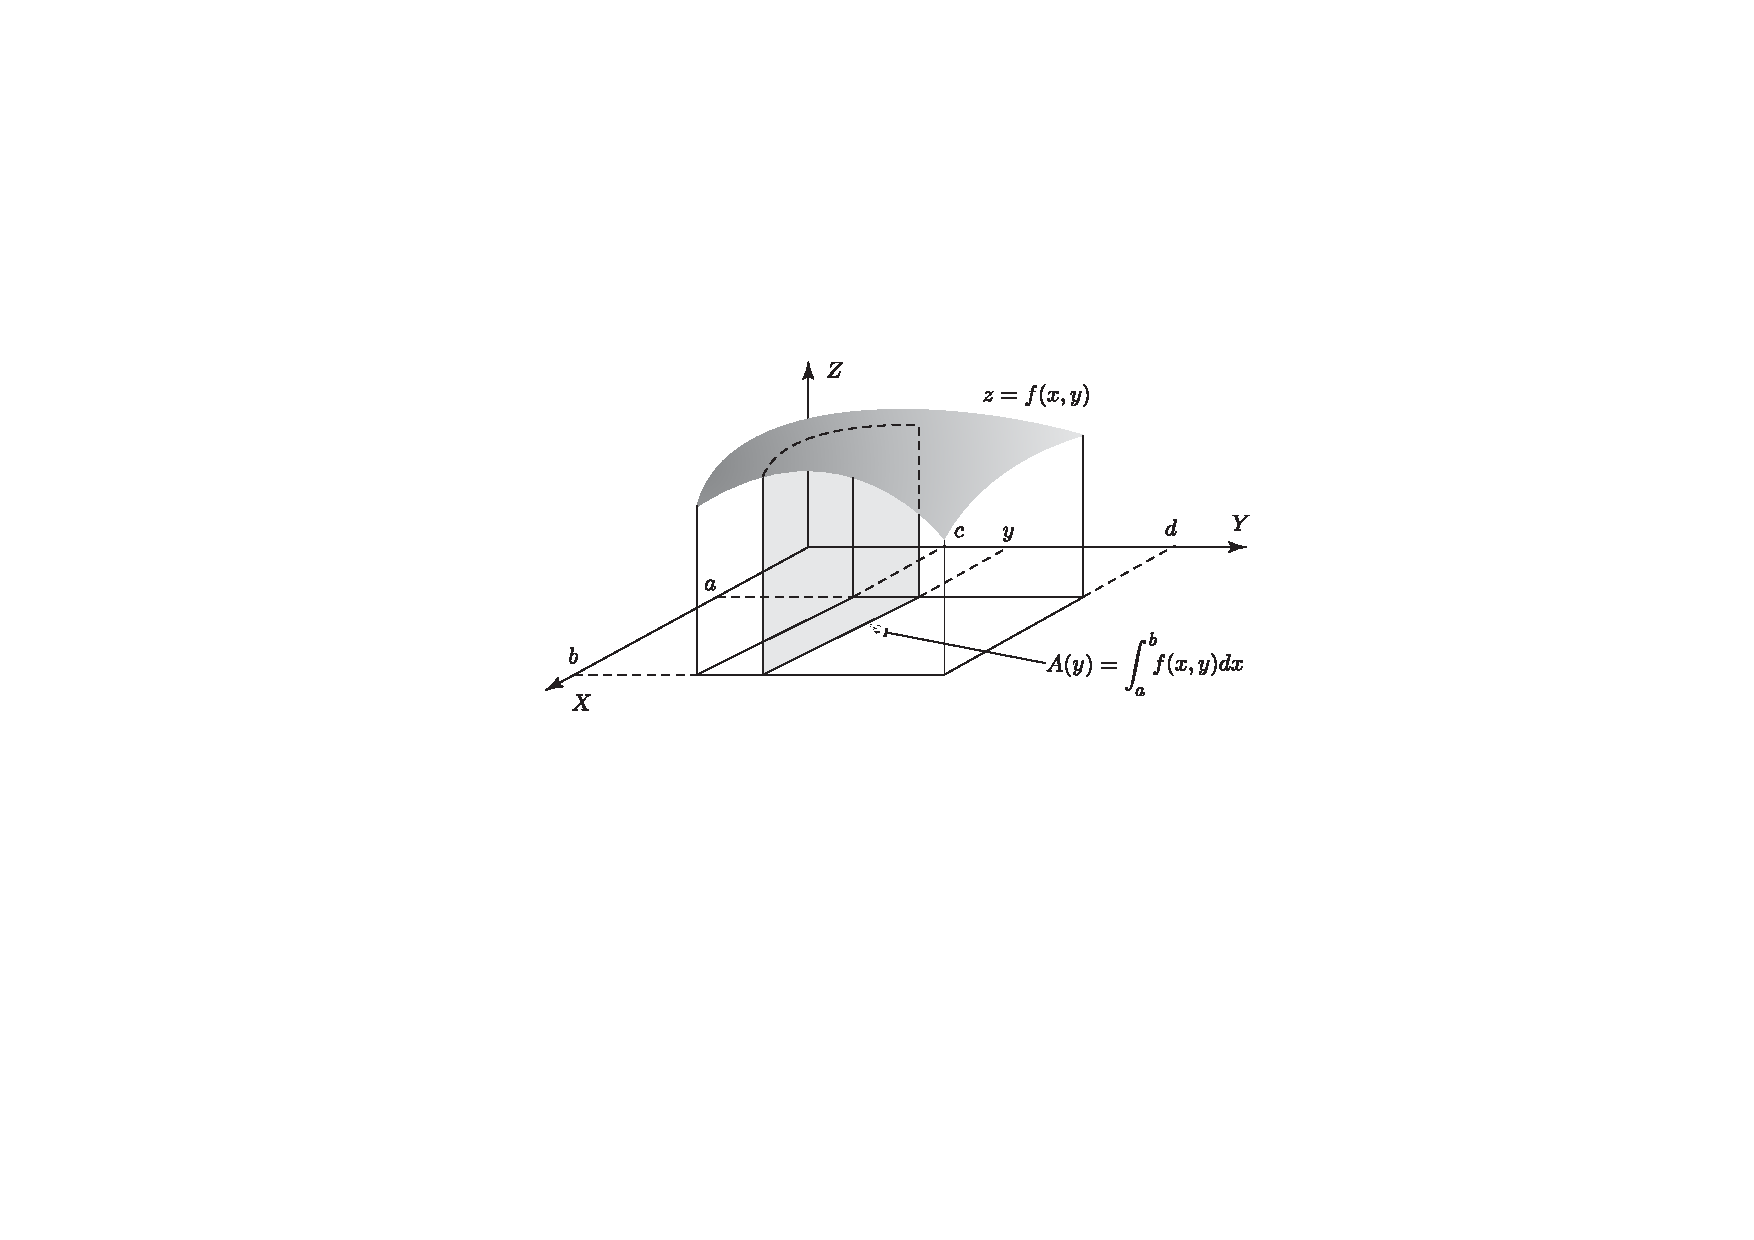
\includegraphics[width=.8\textwidth]{T3/figs/FubIntroY.pdf}\\
$\displaystyle\iint\limits_R f(x,y) = V = \int_c^d A(y)\mathrm dy = \int_c^d \left(\int_a^b f(x,y)\mathrm dx\right)\mathrm dy$
\end{center}
\caption{Justificación del teorema de Fubini usando el cálculo de volúmenes por el método de las secciones.}\label{fig:fub-sec}
\end{figure}
\end{latexonly}

\begin{teorema}[de Fubini]
Sea $f\colon R\subset\mathbb{R}^2\to \mathbb{R}$ un campo escalar integrable en el rectángulo $R=[a,b]\times[c,d]$.
Entonces:
\[
\iint\limits_R f(x,y)\mathrm dx \mathrm dy
=\int_{a}^{b}\left(\int_{c}^{\mathit d}f(x,y)\mathrm dy\right)\mathrm dx
=\int_{c}^{\mathit d}\left(\int_{a}^{b}f(x,y)\mathrm dx\right)\mathrm dy
\]
\end{teorema}
\begin{rawhtml}
&nbsp;
\end{rawhtml}
\begin{ejemplo}
Vamos a calcular la integral $\displaystyle\int_R(2x+y)\mathrm dx\mathrm dy$ con $R=[0,1]\times[0,1]$
%, que estudiamos en la sección anterior haciendo uso de sumas de Riemann.
\begin{align*}
\iint_R(2x+y)\mathrm dx\mathrm dy &= \int_0^1\left(\int_0^1 (2x+y)\mathrm dx\right)\mathrm dy \\
&= \int_0^1 \left[x^2+yx\vphantom{\dfrac12}\right]_{x=0}^1\mathrm dy \\
&= \int_0^1 (1+y)\mathrm dy = \left[y+\frac{y^2}{2}\right]_{y=0}^1=\frac32\tag*{\fej}
\end{align*}
\end{ejemplo}

Como podemos ver en las figuras de la página~\pageref{fig:fub-sec}, las igualdades dadas por el Teorema de Fubini se pueden obtener como consecuencia del método de las secciones para el cálculo de un volumen por el método de las secciones.
\begin{rawhtml}
<div class="center">
<img src="./T3/figuras/Leccion34-3-FubIntroX.svg" width="450">
</div>
<div class="center">
<img src="./T3/figuras/Leccion34-4-FubIntroY.svg" width="450">
</div>
\end{rawhtml}


Naturalmente, trabajar con dominios rectangulares es una restricción demasiado fuerte;
el siguiente resultado introduce la herramienta para trabajar con campos en cualquier dominio.
%
\begin{teorema}\label{th:barf}
Sea $D$ un subconjunto acotado de $\mathbb{R}^2$ y sea $f$ un campo escalar continuo y acotado en $D$. Sea $R$ un rectángulo tal que $D\subset R$ y consideremos el campo
\[
\bar{f}(x,y)=\begin{cases}
f(x,y) & \text{ si } (x,y)\in D\\
0 & \text{ si } (x,y)\in R\smallsetminus D
\end{cases}
\]
Entonces, el campo $\bar f$ es integrable en $R$ y su integral se toma como definición de la integral de $f$ en $D$:
\[
\iint\limits_D f(x,y)\,\mathrm dx\,\mathrm dy \stackrel{(\mathrm{def.})}{=} \iint\limits_R \bar{f}(x,y)\,\mathrm dx\,\mathrm dy
\]
\end{teorema}
\begin{rawhtml}
&nbsp;
\end{rawhtml}
\begin{ejemplo}
Supongamos que $\mathit D\subset\mathbb{R}^2$ está limitado por los grafos de las funciones
$\varphi_1\colon [a,b]\to\mathbb{R}$ y $\varphi_2\colon [a,b]\to\mathbb{R}$ tal y como se muestra en la
figura~\ref{fig:fub}, entonces, considerando la función $\bar{f}$ definida en el
teorema anterior:
\begin{rawhtml}
<div class="center">
<img src="./T3/figuras/Leccion34-5-Fub2.svg" width="300">
</div>
\end{rawhtml}
\begin{align*}
\iint\limits_{\mathit D} f(x,y)\mathrm dx\,\mathrm dy & 
=\int_a^b\left(\int_c^{\mathit d}\bar{f}(x,y)\mathrm dy\right)\mathrm dx\\
& =\int_a^b\left(\int_c^{\varphi_1(x)}0\cdot \mathrm dy+
\int_{\varphi_1(x)}^{\varphi_2(x)}f(x,y) \mathrm dy+\int_{\varphi_2(x)}^{\mathit d}0\cdot \mathrm dy\right)\mathrm dx \\
& =\int_a^b\left(\int_{\varphi_1(x)}^{\varphi_2(x)}f(x,y)\mathrm dy\right)\mathrm dx
\end{align*}
%
\begin{latexonly}
\begin{figure}
\begin{center}
\includegraphics{T3/figs/Fub2.pdf}\\
\end{center}
\caption{Región limitada por dos grafos.}\label{fig:fub}
\end{figure}
\end{latexonly}
%
Por ejemplo, podemos calcular el volumen de la cuña que vimos en un ejemplo anterior, que se obtenía cortando un tronco (cilíndrico) de radio 2 dm dando dos cortes con una sierra mecánica que llegan hasta el centro del
tronco; uno de los cortes se hace perpendicular y el otro formando un ángulo de
$30^\circ$ con  el primero:
\begin{latexonly}
\begin{center}
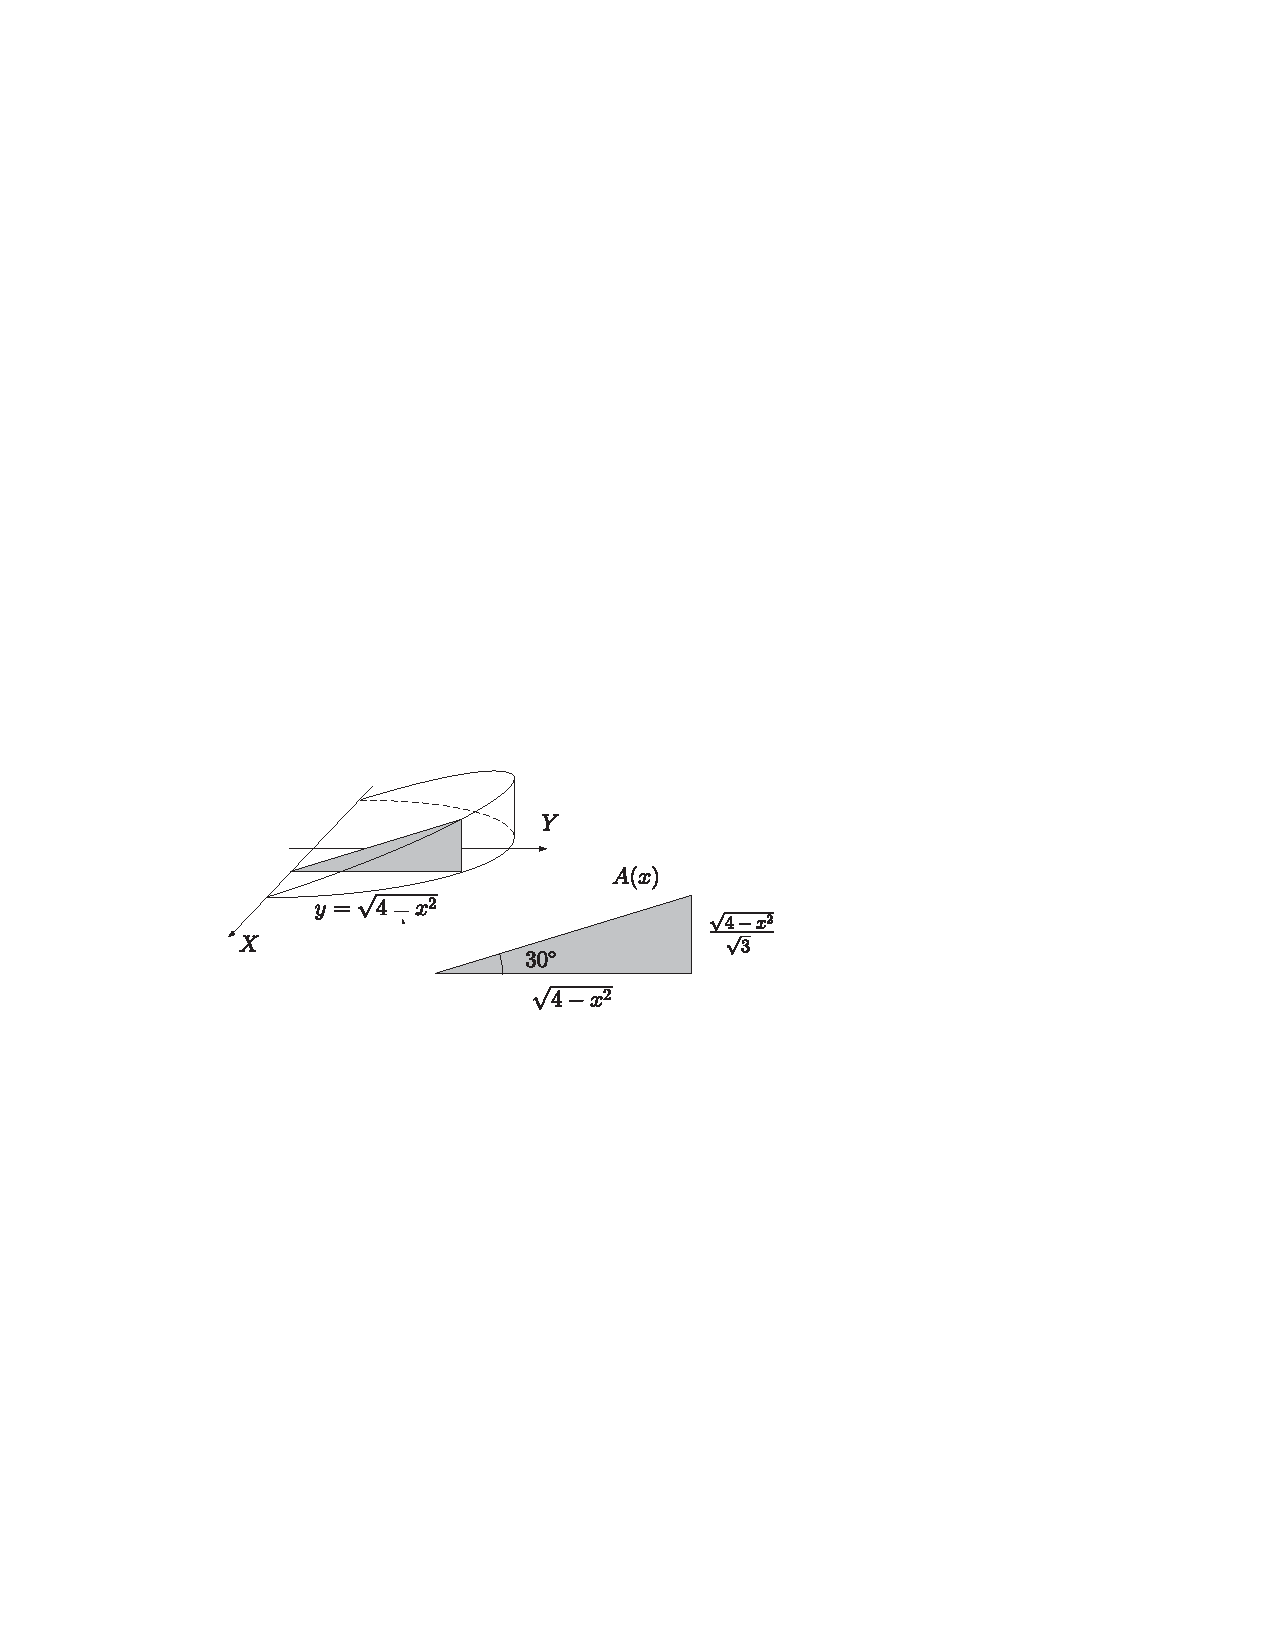
\includegraphics{T3/figs/cunna.pdf}
\end{center}
\end{latexonly}
\begin{rawhtml}
<div class="center">
<img src="./T3/figuras/Leccion33-8-cunna.svg" width="450">
</div>
\end{rawhtml}
Ahora, utilizando una integral doble, la cuña es la región que queda entre el grafo del campo $f(x,y)=\dfrac{y}{\sqrt3}$ y el plano $OX$ en el dominio $\mathit D$ definido por $-2\le x\le 2$, $0\le y \le\sqrt{4-x^2}$.
\begin{align*}
V=&\iint_{\mathit D} \frac{y}{\sqrt3}\,\mathrm dx\,\mathrm dy 
= \int_{-2}^2 \left(\int_0^{\sqrt{4-x^2}} \frac{y}{\sqrt3}\,\mathrm dy\right)\mathrm dx \\
=&\int_{-2}^2 \left[\dfrac{y^2}{2\sqrt3} \right]_0^{\sqrt{4-x^2}}\mathrm dx
= \dfrac{1}{2\sqrt3} \int_{-2}^2  (4-x^2)\mathrm dx\\
= &\dfrac{1}{2\sqrt3} \left[4x-\dfrac{x^3}3\right]_{-2}^2 = \dfrac{16}9\sqrt3\tag*{\fej}
\end{align*}
\end{ejemplo}

Los siguientes resultados establecen varias propiedades de la integral doble.
%
\begin{teorema}
Consideremos un campo escalar $f\colon \mathit{D}\subset\mathbb{R}^2\to \mathbb{R}$ y
supongamos que $f$ es positivo y acotado en $\mathit{D}$.
Entonces, la integral $\int_{\mathit{D}} f(x,y)$ es el valor del volumen del sólido comprendido entre el grafo de $f$ en $\mathit{D}$ y el plano $XY$.
\end{teorema}

Si en este teorema consideramos la función constante $f(x,y)=1$, obtenemos la siguiente consecuencia.

\begin{corolario}\label{cor:areaplana}
$\displaystyle\iint_{\mathit{D}}\,\mathrm dx\,\mathrm dy$ es el valor del área de la región $\mathit D$.
\end{corolario}

La integral doble, también verifica las propiedades de linealidad y de aditividad.

\begin{teorema} Sean $f$ y $g$ campos escalares integrables sobre $\mathit D\subset\mathbb{R}^2$ y
$c,k\in\mathbb{R}$.
\begin{enumerate}
\item Linealidad:
\[\displaystyle\iint\limits_{\mathit D} (c\cdot f(x,y)+k\cdot g(x,y))\,\mathrm dx\,\mathrm dy = c\cdot\Bigg(\iint\limits_{\mathit D} f(x,y)\,\mathrm dx\,\mathrm dy\Bigg)+k\cdot\Bigg(\iint\limits_{\mathit D} g(x,y)\,\mathrm dx\,\mathrm dy\Bigg)
\]
\item Aditividad: Si ${\mathit D}=D_1\cup D_2$ y $\textrm{Área}(D_1\cap D_2) = 0$,
\[
\iint\limits_{\mathit D} f\,\mathrm dx\,\mathrm dy = \Bigg(\iint\limits_{D_1} f(x,y)\,\mathrm dx\,\mathrm dy\Bigg)+\Bigg(\iint\limits_{D_2} f(x,y)\,\mathrm dx\,\mathrm dy\Bigg)
\]
\end{enumerate}
\end{teorema}

\vspace{2em}

\subsection{Teorema de cambio de variable}

El teorema de Fubini es la herramienta fundamental para el cálculo de integrales múltiples, sin embargo, hemos podido observar que su aplicación no es sencilla si la región de integración no es rectangular.
Los cambios de variable nos van a permitir utilizar descripciones más simples de una región. Por ejemplo, mientras que un círculo de radio $a$ centrado en $(0,0)$ en coordenadas cartesianas se describe por $-\sqrt{a^2-x^2}\le y\le \sqrt{a^2-x^2}$, $-a\le x\le a$, en coordenadas polares se describe simplemente por $0\le r\le a$, $0\le \theta\le 2\pi$.
%
\begin{latexonly}
\begin{figure}
\begin{center}
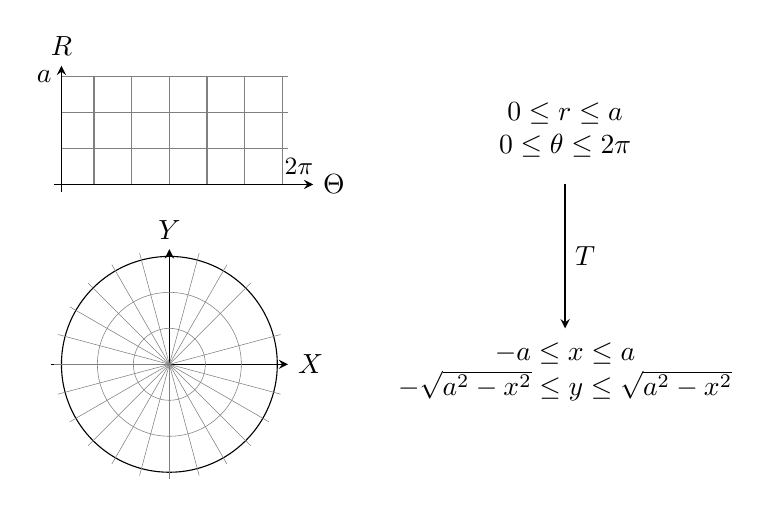
\begin{tikzpicture}[x=1.3em,y=1.3em]
\pgfsetlinewidth{.5pt}
\pgfsetcolor{gray}
\pgfpathgrid[step={\pgfpointxy{1.0472}{1}}]%
{\pgfpointxy{-3}{5}}{\pgfpointxy{3.3}{8}}
\pgfusepath{stroke}
\pgfsetcolor{black}
\draw[-stealth] (-3.2,5) -- (4,5) node[right] {$\Theta$}; 
\draw[-stealth] (-3,4.8) -- (-3,8.3) node[above] {$R$};
\draw (-3,8) node[left] {$a$};
\draw (3.6,5) node[above] {\small $2\pi$};
\draw[-stealth] (-3.3,0) -- (3.3,0) node[right] {$X$}; 
\draw[-stealth] (0,-3.1) -- (0,3.2) node[above] {$Y$};
\draw[thin] (0,0) circle (3);
\foreach \radio in {1,2}
\draw[very thin,color=gray] (0,0) circle (\radio);
%
\foreach \angulo in {15,45,60,75,105,120,135,150,165,180,%
195,210,225,240,255,270,285,300,315,330,345}
\draw[very thin,color=gray] (0,0) -- (\angulo:3.2);
\draw (11,6.5) node{$\begin{array}{c}
0\le r\le a\\
0\le \theta \le 2\pi
\end{array}$};
\draw[-stealth] (11,5) -- (11,1);
\draw (11,3) node[right]{$T$};
\draw (11,-.2) node{$\begin{array}{c}
-a \le x \le a\\
-\sqrt{a^2-x^2}\le y \le \sqrt{a^2-x^2}
\end{array}$};
\end{tikzpicture}
\end{center}
\caption{Cambio de variable a coordenadas polares.}\label{fig:pol}
\end{figure}
\end{latexonly}
%
Para hacer esta descripción alternativa, hemos usado la aplicación
\[
\boldsymbol{T}(r,\theta) = (r\cos\theta,r\operatorname{sen}\theta)
\]
que convierte las \emph{coordenadas polares} en \emph{coordenadas cartesianas}, según se muestra
en la figura~\ref{fig:pol}.
\begin{rawhtml}
<div class="center">
<img src="./T3/figuras/Leccion34-6.svg" width="500">
</div>
\end{rawhtml}
Esta aplicación tiene su origen e imagen en $\mathbb{R}^2$, es decir, es un \emph{campo vectorial}.
Para poder enunciar el teorema de cambio de variable necesitamos introducir algunos conceptos previos.

\begin{definicion} Un campo vectorial es una aplicación cuyo dominio está contenido en un
espacio $\mathbb{R}^n$ y su imagen lo está en otro espacio $\mathbb{R}^m$; es decir, responde al esquema
$\boldsymbol{f}\colon \mathit D\subset\mathbb{R}^n\to \mathbb{R}^m$. Un campo vectorial está determinado por $m$ campos
escalares: $\boldsymbol{f}=(f_1,\dots ,f_m)$.
\end{definicion}

En el teorema de cambio de variable, utilizaremos campos vectoriales continuos y diferenciables, es decir, sus componentes son campos escalares continuos y diferenciables.
La \emph{diferencial} de estos campos se puede estudiar formalmente siguiendo un esquema similar al utilizado para los campos escalares, llegando a la conclusión de que la matriz de esta aplicación lineal se puede expresar a partir de los gradientes de sus componentes según establece la siguiente definición.
Los detalles de estas comprobaciones quedan fuera de los objetivos del curso y de las necesidades de este tema.
%
\begin{definicion}
Si $\boldsymbol{f}=(f_1,\dots,f_m)$ es diferenciable en $\boldsymbol{a}\in \mathrm{Dom}(f)$, llamamos \emph{matriz jacobiana} de $\boldsymbol{f}$ en $\boldsymbol{a}$ a la matriz:
\[
J\boldsymbol{f}(a)=\left(\begin{array}{cccc}
\dfrac{\partial f_1}{\partial x_1}(\boldsymbol{a}) &
\dfrac{\partial f_1}{\partial x_2}(\boldsymbol{a}) & \dots &
\dfrac{\partial f_1}{\partial x_n}(\boldsymbol{a})\\
\dfrac{\partial f_2}{\partial x_1}(\boldsymbol{a}) & 
\dfrac{\partial f_2}{\partial x_2}(\boldsymbol{a}) & \dots & 
\dfrac{\partial f_2}{\partial x_n}(\boldsymbol{a})\\
\vdots & \vdots & \ddots &\vdots \\
\dfrac{\partial f_m}{\partial x_1}(\boldsymbol{a}) & 
\dfrac{\partial f_m}{\partial x_2}(\boldsymbol{a}) & \dots & 
\dfrac{\partial f_m}{\partial x_n}(\boldsymbol{a})
\end{array}\right)_{m\times n}
=\left(\begin{array}{c}
\nabla f_1(\boldsymbol{a})\\
\nabla f_2(\boldsymbol{a})\\
\vdots \\
\nabla f_m(\boldsymbol{a})
\end{array}\right)
\]
\end{definicion}
\begin{rawhtml}
&nbsp;
\end{rawhtml}
\begin{ejemplo}
Vamos a calcular la matriz jacobiana del campo vectorial
\begin{align*}
\boldsymbol f(x,y,z) & =
(3x^2-y,2xz-3y,x-yz^2) \\
J\boldsymbol{f}(x,y,z) & =
\begin{pmatrix}
6x & -1 & 0 \\
2z & -3 & 2x \\
1 & -z^2 & -2yz
\end{pmatrix}\tag*{\fej}
\end{align*}
\end{ejemplo}
Ya tenemos los elementos necesarios para enunciar el teorema de cambio de variable.
%
\begin{teorema} Sea $F\colon \boldsymbol{T}(\mathit D)\subset\mathbb{R}^2\to\mathbb{R}$ un campo escalar continuo, siendo $\mathit D$ cerrado y acotado. Sea $\boldsymbol{T}\colon\mathit D\subset\mathbb{R}^2\to\mathbb{R}^2$ un campo vectorial biyectivo, salvo en un subconjunto de área nula, diferenciable y con las derivadas parciales continuas.
Entonces:
\[
\iint\limits_{\boldsymbol{T}(\mathit D)} F = \iint\limits_{\mathit D} (F\circ \boldsymbol{T})|\det(J\boldsymbol{T})|
\]
\end{teorema}
%
Mientras que para las integrales de una variable, este teorema se utiliza
fundamentalmente para el cálculo de primitivas para simplificar la función a integrar, en la integración múltiple lo utilizaremos fundamentalmente para describir de forma más sencilla la región de integración.

\begin{ejemplo}
Hemos mostrado más arriba el cambio a coordenadas polares:
\[
\boldsymbol{T}(r,\theta) = (r\cos\theta,r\operatorname{sen}\theta)
\]
Veamos como se transforma una integral al aplicar este cambio de variables.
En primer lugar, calculamos el jacobiano de $\boldsymbol{T}$:
\[
J\boldsymbol{T}(r,\theta)=\left(\begin{array}{cc}
\cos\theta & -r\operatorname{sen}\theta\\
\operatorname{sen}\theta & r\cos\theta
\end{array}
\right)
\]
Por lo tanto, el valor absoluto del determinante es: $|\det(J\boldsymbol{T}(r,\theta))| = |r|$;
y la fórmula de cambio de variable queda:
\[
\iint\limits_{\boldsymbol{T}(\mathit D)} F(x,y)\mathrm dx\,\mathrm dy = \iint\limits_{\mathit D} F(r\cos\theta,r\operatorname{sen}\theta)|r|dr\,d\theta
\]
En la integral de la izquierda, $\boldsymbol{T}(\mathit D)$ representa a la región de integración descrita en coordenadas cartesianas, mientras que $\mathit D$, en la integral de la derecha, representa a la misma región pero descrita en coordenadas polares.\fej
\end{ejemplo}
\begin{rawhtml}
&nbsp;
\end{rawhtml}
\begin{ejemplo}\label{ej:reg-paras}
Calculemos la integral $\displaystyle\iint_{D} xy\,\mathrm dx\mathrm dy$ en donde 
$D$ es la región delimitada por las parábolas,
$y=x^2+4, y=x^2, y=6-x^2, y=12-x^2$, según se muestra en la figura~\ref{fig:reg-paras}
\begin{rawhtml}
<div class="center">
<img src="./T3/figuras/Leccion34-8-region.svg" width="220">
</div>
\end{rawhtml}
\begin{latexonly}
\begin{figure}
\begin{center}
\includegraphics{T3/figs/region.pdf}
\end{center}
\caption{Región de integración en el ejemplo~\ref{ej:reg-paras}.}\label{fig:reg-paras}
\end{figure}
\end{latexonly}
En este caso, cada par $(u,v)$ tal que $u\in[6,12]$, $v\in[0,4]$, determina un único punto de la región, determinado por las siguientes ecuaciones
\[
y=x^2+v,\quad  y=u-x^2
\]
Esto permite obtener un cambio de variable de $[6,12]\times [0,4]$ en $D$:
\[
x=\sqrt{\frac12(u-v)},\qquad y=\frac12(u+v)
\]
Utilizamos entonces el cambio $\boldsymbol{T}(u,v)=(\sqrt{\frac12(u-v)},\frac12(u+v))$, para calcular la integral propuesta
\[
\mathrm{Det}(J\boldsymbol{T}(u,v))=\left|\begin{matrix}
\dfrac{\sqrt2}{4\sqrt{u-v}} & \dfrac{-\sqrt2}{4\sqrt{u-v}} \\
\dfrac12 & \dfrac12
\end{matrix}\right| = \dfrac{\sqrt2}{4\sqrt{u-v}}
\]
\begin{multline*}
\iint\limits_{D} xy\,\mathrm dx\mathrm dy =
\iint\limits_{T^{-1}(D)} \dfrac{\sqrt{u-v}(u+v)}{2\sqrt2}\dfrac{\sqrt2}{4\sqrt{u-v}}\mathrm du\,\mathrm dv\\ =
\dfrac{1}{8}\int_0^4\int_6^{12}(u+v)\mathrm du\,\mathrm dv
=\dfrac18\int_0^4\left[\dfrac{u^2}{2}+vu\right]_{u=6}^{12}\mathrm dv\\
=\dfrac18\int_0^4(54+6v)\mathrm dv
=\dfrac18\left[54v+3v^2\vphantom{\dfrac12}\right]_{v=0}^{4}\mathrm dv 
= 33\tag*{\fej}
\end{multline*}
\end{ejemplo}

%\subsection{Aplicaciones}

%Tal y como ocurre con las funciones de variable real, las aplicaciones de la integral doble no se reducen al cálculo de volúmenes. Son múltiples las magnitudes físicas, matemáticas y de otras áreas que pueden ser modeladas y calculadas con este tipo de integrales. A modo de ejemplo, mostramos dos aplicaciones geométricas.

\subsection{Áreas de regiones planas}

Según hemos visto anteriormente, la integral doble nos da una forma sencilla de expresar el área de una región plana arbitraria:
\[
\mathrm{\acute{A}rea}(\mathit D)=\iint\limits_{\mathit D} \mathrm dx\mathrm dy,
\]
El uso de las técnicas presentadas en las secciones anteriores nos permitirá abordar el cálculo del área de regiones cuyas representaciones como integrales de una variable sería más compleja.

\begin{ejemplo}
Calculemos el área de la región interior a la elipse $\dfrac{x^2}{a^2}+\dfrac{y^2}{b^2}=1$.
%\[
%\mathrm{\acute{A}rea}(D)=\int\limits_D \mathrm dx\mathrm dy.
%\]
Podemos plantear la integral en la región elíptica aplicando directamente el teorema de Fubini, pero las primitivas resultantes no serán sencillas.
Es mejor utilizar un cambio de variable, que podemos intuir fácilmente si recordamos la parametrización de la elipse que estudiamos en el tema~2:
\[
\frac{x}a =r \cos t,\qquad \frac{y}b=r\operatorname{sen} t,\quad r\in[0,1],\quad t\in[0,2\pi].
\]
Obsérvese que este cambio no es el cambio a coordenadas polares; de hecho, el uso de coordenadas polares sobre regiones elípticas conduce, por lo general, a primitivas más complejas.

Por lo tanto:
\begin{align*}
\boldsymbol{T}(r,t) &= (ar\cos t,br\operatorname{sen} t) \\
J\boldsymbol{T}(r,t) &=
\begin{pmatrix}
a\cos t & -ar\operatorname{sen} t \\
b\operatorname{sen} t & br\cos t
\end{pmatrix} \\
|\mathrm{Det}(J\boldsymbol{T}(r,t))| & = rab \\
\mathrm{\acute{A}rea}(\mathit D)&=\iint\limits_{\mathit D} \mathrm dx\mathrm dy=\int_0^{2\pi}\int_0^1 abr\,dr\,\mathrm dt =\pi ab\tag*{\fej}
\end{align*}
\end{ejemplo}


%
%\paragraph{Áreas de grafos.} Si $f$ es un campo escalar continuo con parciales continuas en un dominio~$\mathit D$, entonces el área de la superficie de su grafo sobre el dominio $\mathit D$ es
%\[
%\int\limits_{\mathit D} \sqrt{1+\Big(\dfrac{\partial f}{\partial x}(x,y)\Big)^2+
%\Big(\dfrac{\partial f}{\partial y}(x,y)\Big)^2}\,\mathrm dx\,\mathrm dy
%\]
%La expresión del integrando se conoce como \emph{diferencial de superficie} y juega un papel similar al de la diferencial de longitud.
%
%%:Arreglar: Pasar integral de línea a la lección anterior y dejar aquí solo
%% el teorema de Green.

\subsection{Integrales de línea}

Una de las aplicaciones fundamentales de la integral en la física es el cálculo del trabajo que realiza un campo (vectorial) de fuerzas al desplazarse por una curva. 
Esta magnitud se modeliza con lo que se conoce como \emph{integral de línea}, que definimos a continuación.
%
\begin{definicion}
Sea $\boldsymbol{F}=(F_1,F_2)$ un campo vectorial y $\gamma(t)$, $t\in[a,b]$, una curva en $\mathbb{R}^2$ tal que $\gamma'$ es continua en $[a,b]$.
Llamamos \emph{integral de línea de $\boldsymbol{F}$ sobre la curva $C$} o \emph{circulación de $\boldsymbol{F}$ a través de $C$}~a:
\[
\int_C \boldsymbol{F} = 
\int_a^b \boldsymbol{F}(\gamma(t))\cdot\gamma'(t)\,\mathrm dt
= \int_a^b (F_1(x(t),y(t))x'(t)+F_2(x(t),y(t))y'(t))\,\mathrm dt
\]
Si la curva $C$ es cerrada, es decir $\gamma(a)=\gamma(b)$, esta integral se denota:
$\displaystyle\oint_C \boldsymbol{F}$
\end{definicion}
De forma más abreviada, la integral de línea se suele expresar igualmente como sigue:
\[
\int_C \boldsymbol{F} = \int_C F_1(x,y)\mathrm dx+F_2(x,y)\mathrm dy
\]

\begin{latexonly}
\begin{figure}
\begin{center}
\begin{tikzpicture}[x=30em,y=30em]
\draw[domain=0:.1,smooth,variable=\t,-stealth]
plot (2*\t*\t*\t-3*\t*\t+\t,\t-\t*\t);
\draw[domain=.1:.3,smooth,variable=\t,-stealth]
plot (2*\t*\t*\t-3*\t*\t+\t,\t-\t*\t);
\draw[domain=.3:.6,smooth,variable=\t,-stealth]
plot (2*\t*\t*\t-3*\t*\t+\t,\t-\t*\t);
\draw[domain=.6:.9,smooth,variable=\t,-stealth]
plot (2*\t*\t*\t-3*\t*\t+\t,\t-\t*\t);
\draw[domain=.9:1,smooth,variable=\t]
plot (2*\t*\t*\t-3*\t*\t+\t,\t-\t*\t);
% Ejes
\draw[-stealth] (-.16,0) -- (.16,0) node[right] {$X$}; 
\draw[-stealth] (0,-.01) -- (0,.3) node[right] {$Y$};;
\end{tikzpicture}
\end{center}
\caption{Curva de los ejemplos~\ref{ej:int-lin} y~\ref{ej:area-green}.}\label{fig:ej-int-lin}
\end{figure}
\end{latexonly}
\begin{ejemplo}\label{ej:int-lin}
Consideremos el campo $\boldsymbol F(x,y)=\Big(\dfrac{x}{y},\dfrac{y}x\Big)$ y la curva cerrada $C$ determinada por la parametrización
$\gamma(t)=(2t^3-3t^2+t,t-t^2)$, $t\in[0,1]$ (ver figura~\ref{fig:ej-int-lin}).
\begin{rawhtml}
<div class="center">
<img src="./T3/figuras/Leccion34-9.svg" width="250">
</div>
\end{rawhtml}
\begin{multline*}
\oint_{C} \boldsymbol{F} = 
\int_0^1 \boldsymbol{F}(\gamma(t))\cdot\gamma'(t)\,\mathrm dt
= \int_0^1 (F_1(x(t),y(t))x'(t)+F_2(x(t),y(t))y'(t))\,\mathrm dt =\\
= \int_0^1 \left(\frac{x(t)}{y(t)}x'(t)+\frac{y(t)}{x(t)}y'(t)\right)\,\mathrm dt =\\
= \int_0^1 \left(\frac{t(t-1)(2t-1)}{-t(t-1)}(6t^2-6t+1)+
\frac{-t(t-1)}{t(t-1)(2t-1)}(1-2t)\right)\,\mathrm dt =\\
= \int_0^1 \big(-(2t-1)(6t^2-6t+1)+1\big)\,\mathrm dt =\\
= \int_0^1 (-12t^3+18t^2-8t+2)\,\mathrm dt =\\
= \left[-3t^4+6t^3-4t^2+2t\right]_0^1=-3+6-4+2=1\tag*{\fej}
\end{multline*}
\end{ejemplo}

Las integrales de línea y las integrales dobles están relacionadas por el teorema de Green, que enunciamos a continuación.
%
\begin{teorema}[de Green]\label{th:green}
Sea $C$ es una curva regular a trozos, cerrada y simple de $\mathbb{R}^2$ recorrida de tal forma que el interior de la curva queda a la izquierda,~$\mathit D$ la región interior de esta curva y
$\boldsymbol{F}\colon \mathit D\subset\mathbb{R}^2\to\mathbb{R}^2$ un campo vectorial continuo y con parciales continuas en~$\mathit D$.
Entonces
\[
\oint_C \boldsymbol{F}  =  \int\limits_{\mathit D} \Big(\dfrac{\partial F_2}{\partial x}(x,y) - \dfrac{\partial F_1}{\partial y}(x,y)\Big)\,\mathrm dx\,\mathrm dy
\]
\end{teorema}

\begin{latexonly}
\begin{figure}
\begin{center}
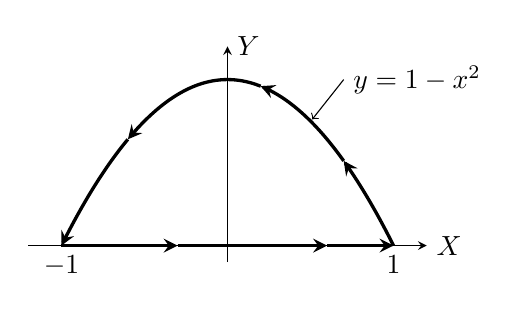
\begin{tikzpicture}[x=6em,y=6em]
\draw[very thick,domain=0:.3,smooth,variable=\t,-stealth]
plot (1-\t,-\t*\t+2*\t);
\draw[very thick,domain=.3:.8,smooth,variable=\t,-stealth]
plot (1-\t,-\t*\t+2*\t);
\draw[very thick,domain=.8:1.6,smooth,variable=\t,-stealth]
plot (1-\t,-\t*\t+2*\t);
\draw[very thick,domain=1.6:2,smooth,variable=\t,-stealth]
plot (1-\t,-\t*\t+2*\t);
\draw[very thick,-stealth] (-1,0)--(-.3,0);
\draw[very thick,-stealth] (-.3,0)--(.6,0);
\draw[very thick,-stealth] (.6,0)--(1,0);
\draw[<-] (.51,.76)--(.7,1) node[right]{$y=1-x^2$};
\draw (-1,0) node[below]{$-1$};
\draw (1,0) node[below]{$1$};
% Ejes
\draw[-stealth] (-1.2,0) -- (1.2,0) node[right] {$X$}; 
\draw[-stealth] (0,-.1) -- (0,1.2) node[right] {$Y$};;
\end{tikzpicture}
\end{center}
\caption{Curva del ejemplo~\ref{ej:green}.}\label{fig:ej-green}
\end{figure}
\end{latexonly}
\begin{ejemplo}\label{ej:green}
Vamos a calcular la integral del campo $\boldsymbol F(x,y)=(y^2,x^2)$ sobre la curva cerrada $C$ que aparece en la figura~\ref{fig:ej-green}; 
\begin{rawhtml}
<div class="center">
<img src="./T3/figuras/Leccion34-10.svg" width="300">
</div>
\end{rawhtml}
esta curva está formada por el segmento que une los puntos $(-1,0)$ y $(1,0)$ y el segmento de la parábola $y=1-x^2$ que va de $(1,0)$ a $(-1,0)$.
Dado que vamos a utilizar el teorema de Green, no es necesario obtener una parametrización.
Si $\mathit{D}$ es la región encerrada por la curva: 
\begin{multline*}
\oint_{C} \boldsymbol{F} = 
\oint_{C} y^2\,\mathrm dx + x^2\,\mathrm dy =
\iint\limits_{\mathit D} (2x-2y)\,\mathrm dx\,\mathrm dy =\\
=\int_{-1}^1 \int_0^{1-x^2} (2x-2y)\,\mathrm dy\,\mathrm dx =
\int_{-1}^1 \left[2xy-y^2\right]_0^{y=1-x^2}\,\mathrm dx =\\
=\int_{-1}^1 2x(1-x^2)-(1-x^2)^2\,\mathrm dx =
\int_{-1}^1 (-x^4-2x^3+2x^2+2x-1)\,\mathrm dx =\\
=\left[-\frac15x^5-\frac12x^4+\frac23x^3+x^2-x\right]_{-1}^1  =\\
=(-\frac15-\frac12+\frac23+1-1)-(\frac15-\frac12-\frac23+1+1) = \frac{-16}{15}\tag*{\fej}
\end{multline*}
\end{ejemplo}

Si $C$ es una curva cerrada y $D$ es la región del plano que encierra, entonces, por el teorema de Green
\[
\oint_{C} -y\,\mathrm dx + x\,\mathrm dy = \iint\limits_{\mathit D} (1-(-1))\,\mathrm dx\,\mathrm dy )= 
2\iint\limits_{\mathit D} \mathrm dx\,\mathrm dy = 2\text{Área}(D)
\]
Hemos considerado que la curva se está recorriendo en sentido positivo, es decir, de tal forma que el interior queda a la izquierda.
Si la curva se recorre en sentido contrario, el valor de la integral será negativo, aunque su valor absoluto coincidirá igualmente con el área.
Este razonamiento demuestra el siguiente corolario.

\begin{corolario}\label{cor:areacurva}
Si $C$ es una curva regular, cerrada y simple, entonces el área de la región encerrada por $C$ es
\[
A= \frac12\left|\oint_C -y\,\mathrm dx+x\,\mathrm dy\right|
\]
\end{corolario}
\begin{rawhtml}
&nbsp;
\end{rawhtml}
\begin{ejemplo}\label{ej:area-green}
Vamos a calcular el área de la región  encerrada por la curva $C$ determinada por la parametrización $\gamma(t)=(2t^3-3t^2+t,t-t^2)$, $t\in[0,1]$ (ver figura~\ref{fig:ej-int-lin}).
\begin{multline*}
\text{Área}=\frac12\oint_{C} -y\,\mathrm dx+x\,\mathrm dy =\\
= \int_0^1 \frac12\big(-(t-t^2)(6t^2-6t+1)+(2t^3-3t^2+t)(1-2t)\big)\,\mathrm dt =\\
= \int_0^1 (t^4-2t^3+t^2)\,\mathrm dt 
= \left[\frac15t^5-\frac12t^4+\frac13t^3\right]_0^1=\frac15-\frac12+\frac13=\frac1{30}\tag*{\fej}
\end{multline*}
\end{ejemplo}


%    \newpage
%    \thispagestyle{empty}
%    
%    \ 
%    
%    \vfill
%    \begin{center}
%    (Esta página se ha dejado intencionalmente en blanco)
%    \end{center}

\newpage

%%%%%%%%%%%%%%%%%%%%%%%%%%%%%%%%%%%%%%%%%%%%%%%%%%%%%%%%%%%%%%%%%%%%%%%%%%%%%%%%%%%%
\section*{Relación de ejercicios \thechapter.1}
%%%%%%%%%%%%%%%%%%%%%%%%%%%%%%%%%%%%%%%%%%%%%%%%%%%%%%%%%%%%%%%%%%%%%%%%%%%%%%%%%%%%

\pagestyle{relaciones}


\begin{enumerate}


\item Las expresiones $\dfrac{1}{x}$ y $\dfrac{2}{2x}$ son iguales, sin embargo, si calculamos la integral (inmediata) de cada una de ellas, obtenemos los siguientes resultados:
\[
\displaystyle\int\frac{1}{x}\,\mathrm dx=\log |x|+C \qquad\text{ y }\qquad \displaystyle\int\frac{2}{2x}\,\mathrm dx=\log|2x| + C
\] 
¿Son esos dos resultados realmente distintos?


\item Calcule las siguientes integrales observando que son inmediatas:

\setcontadoralph
\begin{center}
\begin{tabular}{l@{\qquad\quad}l}
\nitem $\displaystyle\int(4x^3-3x^2+\dfrac{1}{2}x-\pi)\,\mathrm dx$ &
\nitem $\displaystyle\int\sqrt[3]{x^2}\,\mathrm dx$ \\
\nitem $\displaystyle\int\cos x\operatorname{sen}^3 x\,\mathrm dx$ &
\nitem $\displaystyle\int x\operatorname{sen} x^2\,\mathrm dx$
\end{tabular}
\end{center}

\item
\begin{enumerate}
\item
Transforme el polinomio $9x^2-6x+2$ usando la técnica de completar cuadrados.
\item
Utilice la expresión anterior para calcular la integral $\displaystyle\int\dfrac{3}{9x^2-6x+2}\mathrm{d}x$
\end{enumerate}


\item
Utilice la descomposición en fracciones simples para calcular la integral
\[
\int\dfrac{x^2+6x+5}{x^3-x^2-x-2}\mathrm{d}x
\]


\item Calcule las siguientes integrales racionales, analizando en primer lugar si son inmediatas:

\setcontadoralph
\begin{centrar}
\nitem $\displaystyle\int\dfrac{x}{4+x^4}\,\mathrm dx$ \hfill
\nitem $\displaystyle\int\dfrac{x^3}{4+x^4}\,\mathrm dx$ \hfill
\nitem $\displaystyle\int\dfrac{x^2}{4+x^4}\,\mathrm dx$
\end{centrar}

\item Calcule las  integrales 
\setcontadoralph
\begin{centrar}
\nitem $\displaystyle\int\operatorname{tg} x\,\mathrm dx$,\hfill
\nitem $\displaystyle\int(\log x)^2\,\mathrm dx$
\end{centrar}
y deduzca a partir de ellas las integrales siguientes:
\begin{centrar}
\nitem $\displaystyle\int e^x\,\operatorname{tg} e^x\,\mathrm dx$,\hfill
\nitem $\displaystyle\int\dfrac{(\log(\operatorname{arctg} x))^2}{1+x^2}\,\mathrm dx$
\end{centrar}


\item Calcule las  integrales siguientes utilizando el método de integración por partes.
\setcontadoralph
\begin{centrar}
\nitem $\displaystyle\int e^{2x}\cos x\,\mathrm dx$ \hfill
\nitem $\displaystyle\int x^5 \operatorname{sen} x^3\,\mathrm dx$
\end{centrar}

\item
Utilice el cambio de variable $t=e^x$ y las fórmulas de derivación vistas en el tema para calcular la integral
\[
\displaystyle\int\dfrac{\text{e}^x\,\mathrm dx}{1-\text{e}^{2x}}
\]

\item Calcule las siguientes integrales teniendo en cuenta que son funciones racionales en seno y coseno y utilizando el cambio más adecuado según lo explicado en la sección~\ref{trig}.
\setcontadoralph
\begin{centrar}
\nitem $\displaystyle\int\operatorname{sen}^3 x\cos^2 x\,\mathrm dx$ \hfill
\nitem $\displaystyle\int\dfrac{\mathrm dx}{1+\cos x}$
\end{centrar}

\item
Calcule la integral $\displaystyle\int \dfrac{\sqrt{1-x}}{1-\sqrt{x}}\,\mathrm dx$ utilizando en primer lugar el cambio de variable $x=\operatorname{sen}^2 t$ y posteriormente el cambio más adecuado según lo explicado en la sección~\ref{trig}.

\item Consideramos la integral $\displaystyle\int\cos^5 x\,\mathrm dx$:
\begin{enumerate}
\item
Calcúlela utilizando la forma compleja de las funciones trigonométricas.
\item
Calcúlela utilizando el cambio de variable $\operatorname{sen} x=t$.
\end{enumerate}


\item
Resuelva las siguientes integrales irracionales.
\setcontadoralph
\begin{centrar}
\nitem $\displaystyle\int\dfrac{x\,\mathrm dx}{\sqrt{5-4x-x^2}}$ \hfill
\nitem $\displaystyle\int(x-3)\sqrt{x^2-6x}\,\mathrm dx$ 
\end{centrar}

\item
Calcule las siguientes integrales prestando especial atención al indicador de la variable ($\mathrm dx$ o $\mathrm dy$) de integración.
\setcontadoralph
\begin{center}
\begin{tabular}{l@{\qquad\qquad}l@{\qquad\qquad}l}
\nitem $\displaystyle\int x\,\mathrm dx$ &
\nitem $\displaystyle\int 2xy^2\,\mathrm dx$ &
\nitem $\displaystyle\int \dfrac{x}{y^2+x^4}\,\mathrm dx$ \\
\nitem $\displaystyle\int x\,\mathrm dy$ &
\nitem $\displaystyle\int 2xy^2\,\mathrm dy$ &
\nitem $\displaystyle\int\dfrac{x}{y^2+x^4}\,\mathrm dy$
\end{tabular}
\end{center}



\end{enumerate}

%%%%%%%%%%%%%%%%%%%%%%%%%%%%%%%%%%%%%%%%%%%%%%%%%%%%%%%%%%%%%%%%%%%%%%%%%%%%%%%%%%%%
\newpage
%%%%%%%%%%%%%%%%%%%%%%%%%%%%%%%%%%%%%%%%%%%%%%%%%%%%%%%%%%%%%%%%%%%%%%%%%%%%%%%%%%%%
\section*{Relación de ejercicios \thechapter.2}
%%%%%%%%%%%%%%%%%%%%%%%%%%%%%%%%%%%%%%%%%%%%%%%%%%%%%%%%%%%%%%%%%%%%%%%%%%%%%%%%%%%%

\pagestyle{relaciones}


\begin{enumerate}

\item Distinga si las siguientes expresiones son ecuaciones diferenciales y determine el tipo (ordinarias o en derivadas parciales) y el orden.
\setcontadoralph
\begin{center}
\begin{tabular}{l@{\qquad\qquad}l}
\nitem $x^2+3y^2=5xy$ &
\nitem $x^2+3y''-5(y')^3=0$ \\
\nitem $1+y+y''+y'''=0$ &
\nitem $xy-y'\operatorname{sen} x=0$ \\
\nitem $x\dfrac{\mathrm dy}{\mathrm dx}-\operatorname{sen} x = \mbox{e}^x$ &
\nitem $5\left(\dfrac{\partial z}{\partial x}\right)^2+xy\dfrac{\partial z}{\partial y}=3xyz$
\end{tabular}
\end{center}


\item Consideremos la ecuación $y'+2y=0$. Se pide:
\begin{enumerate}
\item Estudie la existencia y unicidad de soluciones.
\item Compruebe que la función $y=Ce^{-2x}$ es una solución general.
\item Determine la solución particular que pasa por el punto $(0,3)$.
\end{enumerate}

\item Consideremos la ecuación diferencial $y'=y^2-4$. Se pide
\begin{enumerate}
\item Estudie la existencia y unicidad de soluciones
\item Resuelva la ecuación (variables separables) y obtener la solución general.
\item Calcule la solución particular, si existe, que pasa por $(0,0)$.
\item Calcule la solución particular, si existe, que pasa por $(0,2)$.
\item Calcule la solución particular, si existe, que pasa por $(0,-2)$.
\end{enumerate}

\item
Compruebe que la ecuación $xyy'-\log x=0$ es de variables separables y resuélvala. ¿Alguna solución pasa por el punto $(1,-2)$?


\item
Compruebe que la ecuación $(2x-3y)+(2y-3x)y'=0$ es exacta y resuélvala.  ¿Alguna solución pasa por el punto $(1,-2)$?


\item
Resuelva la ecuación diferencial lineal
$y'+\dfrac{y}{x}=3x+4$ y compruebe la solución.  ¿Alguna solución pasa por el punto $(2,6)$?



\item
Resuelva la ecuación $y'=\dfrac{xy}{x^2-y^2}$ utilizando el cambio de variable $y=x\cdot u$ y compruebe la solución.

\item
Resuelva la ecuación $yy'-2y^2=e^x$ utilizando el cambio de variable $u=y^2$.

\item
Entre los modelos estudiados en el tema, determine qué tipo de ecuación diferencial es cada una de las siguientes:
\setcontadoralph
\begin{center}
\begin{tabular}{l@{\qquad\quad}l}
\nitem $(2+x)y'=3y$ &  %sep
\nitem $y'=\dfrac{3x+2y}{x}$ \\ %lin
\nitem $2\cos(2x-y)-y'\cos(2x-y)=0$ & %exac
\nitem $y'=-2-y+y^2$ \\ %sep
\nitem $(x-1)y'+y=x^2-1$ & %lin
\nitem $y'=\dfrac{y+x-3}{y-x-1}$ \\ %exac
\nitem $y'+2xy=2x$ & %lin
\nitem $e^xyy'=e^{-y}+e^{-2x-y}$ \\ %sep
\nitem $y'+2y=\operatorname{sen} x$ & %lin
\nitem $y^2e^{xy^2} + 2xyy'e^{xy^2}=0$ %exac
\end{tabular}
\end{center}

\end{enumerate}

%%%%%%%%%%%%%%%%%%%%%%%%%%%%%%%%%%%%%%%%%%%%%%%%%%%%%%%%%%%%%%%%%%%%%%%%%%%%%%%%%%%%
\newpage
\thispagestyle{empty}

\ 

\vfill
%\begin{center}
%(Esta página se ha dejado intencionalmente en blanco)
%\end{center}
\newpage

%%%%%%%%%%%%%%%%%%%%%%%%%%%%%%%%%%%%%%%%%%%%%%%%%%%%%%%%%%%%%%%%%%%%%%%%%%%%%%%%%%%%
\section*{Relación de ejercicios \thechapter.3}
%%%%%%%%%%%%%%%%%%%%%%%%%%%%%%%%%%%%%%%%%%%%%%%%%%%%%%%%%%%%%%%%%%%%%%%%%%%%%%%%%%%%

\pagestyle{relaciones}


\begin{enumerate}


\item
Calcule la siguiente integral utilizando el cambio de variable $x=t^2$.
\[
\displaystyle\int_0^{\pi^2/4}\operatorname{sen}\sqrt{x}\,\mathrm dx
\]

\item
Calcule el área de las regiones acotadas delimitadas por las gráficas de las funciones $f(x)=x^4-9x^2+10$ y
$g(x)=x^2+1$.


%Volumen por discos y capas
\item Consideremos la región comprendida entre la curva $y=x^2$ y la recta $y=x+2$.
Dibuje la región y utilice los modelos de la sección~\ref{sec:geom} para calcular los siguientes volúmenes.
\begin{enumerate}
\item Volumen de revolución que se genera al girar la región alrededor del eje $X=2$.
\item Volumen de revolución que se genera al girar la región alrededor del eje $Y=-1$.
\end{enumerate}


%Longitud de un arco en paramétricas
\item Halle la distancia recorrida por un móvil entre los instantes $t=0$ y $t=4$ si su posición viene determinada por las ecuaciones:
$$ x(t)=\frac{t^2}{2},\qquad y(t)=\frac{1}{3}(2t+1)^{3/2} $$


\item
Halle la integral $\displaystyle\iint\limits_R y^3\cos^2x\,\mathrm dx\,\mathrm dy$, en donde
$R=[-1,2]\times [0,2]$

\item
Halle la integral $\displaystyle\iint\limits_R yx^3 e^{x^2y^2}\,\mathrm dx\,\mathrm dy$, en donde
$R=[1,3]\times [1,2]$


\item Dibuje la región sobre la que se integra, intercambie el orden de
integración y evalúe la integral 
\[
\int_0^1\int_x^1 (x-y)^3\,\mathrm dy\,\mathrm dx.
\]

\item Dibuje la región sobre la que se integra, intercambie el orden de
integración y evalúe la integral 
\[
\int_1^4\int_1^{\sqrt{x}} (x^2+y^2)\,\mathrm dy\,\mathrm dx.
\]

\end{enumerate}

\newpage
\thispagestyle{empty}

\ 

\vfill
%\begin{center}
%(Esta página se ha dejado intencionalmente en blanco)
%\end{center}
%%%%%%%%%%%%%%%%%%%%%%%%%%%%%%%%%%%%%%%%%%%%%%%%%%%%%%%%%%%%%%%%%%%%%%%%%%%%%%%%%%%%
\newpage
%%%%%%%%%%%%%%%%%%%%%%%%%%%%%%%%%%%%%%%%%%%%%%%%%%%%%%%%%%%%%%%%%%%%%%%%%%%%%%%%%%%%
\section*{Relación de ejercicios \thechapter.4}
%%%%%%%%%%%%%%%%%%%%%%%%%%%%%%%%%%%%%%%%%%%%%%%%%%%%%%%%%%%%%%%%%%%%%%%%%%%%%%%%%%%%

\pagestyle{relaciones}


\begin{enumerate}
\item
Consideramos la región $R$ delimitada por las rectas $y=x+1$, $y=x-3$, $y=4-x$, $y=3-x$.
Utilizar el teorema de cambio de variable para expresar la integral respecto de las variables $u$ y $v$ tales que $y=x+u$, $y=v-x$ y calcularla
\[
\iint\limits_R (y-2x)\,\mathrm dx\,\mathrm dy.
\]

\item
Utilice el cambio de variable a coordenadas polares para hallar la integral
\[
\iint\limits_{\mathit D} xy\,\mathrm dx\,\mathrm dy,
\]
en donde $\mathit D$ es el interior de la curva $(x^2+y^2)^2=4(x^2-y^2)$ en $x\geq 0$.

%Area en coordenadas polares
\item
Utilice el cambio de variable a coordenadas polares para hallar el área encerrada por la cardioide de ecuación $\rho=3(1+\cos\theta)$.


\item
Si $f$ es un campo escalar continuo con parciales continuas en un dominio~$\mathit D$, entonces el área de la superficie de su grafo sobre el dominio $\mathit D$ es
\[
\iint\limits_{\mathit D} \sqrt{1+\Big(\dfrac{\partial f}{\partial x}(x,y)\Big)^2+
\Big(\dfrac{\partial f}{\partial y}(x,y)\Big)^2}\,\mathrm dx\,\mathrm dy
\]
Halle el área de la superficie del grafo del campo $f(x,y)=xy$ sobre el círculo de centro $(0,0)$ y radio 1.


\item
Consideramos la siguiente integral de línea:
\[
\oint_C y^3\mathrm dx + (x^3+3xy^2)\mathrm dy
\]
en donde $C$ es la curva que va del punto $(1,1)$ al punto $(0,0)$ siguiendo la recta $Y=X$ y vuelve al punto $(1,1)$ siguiendo la curva $Y=X^3$.
\begin{enumerate}
\item
Calcúlela utilizando la definición.
\item
Calcúlela utilizando el teorema de Green (página~\pageref{th:green}).
\end{enumerate}


\item
Consideramos la parábola de la figura cuya parametrización es $x(t)=t^2+t-2$, $y(t)=-t^2+t+6$, $t\in[-2,3]$.
Calcule el área de la región sombreada de la figura.
\begin{latexonly}
\begin{center}
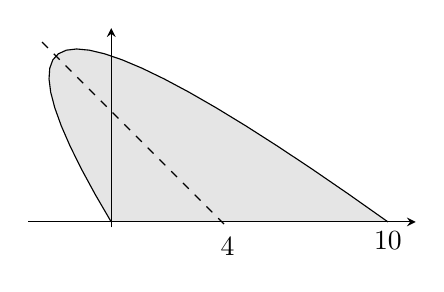
\begin{tikzpicture}[x=1em,y=1em]
\filldraw[domain=-2:3,variable=\t,gray!20] plot (\t*\t+\t-2,-\t*\t+\t+6);
\draw[domain=-2:3,variable=\t] plot (\t*\t+\t-2,-\t*\t+\t+6);
\draw (0,0)--(10,0);
\draw[-stealth] (0,-.2) -- (0,7);% node[right] {$Y$}; 
\draw[-stealth] (-3,0) -- (11,0);% node[above] {$X$};
\draw[dashed] (-2.5,6.5) -- (4.2,-.2) node[below]{$4$};
\draw (10,0) node[below]{$10$};
\end{tikzpicture}
\end{center}
\end{latexonly}
\begin{rawhtml}
<div class="center">
<img src="./T3/figuras/Relacion34-1.svg" width="450">
</div>
\end{rawhtml}

\end{enumerate}

\newpage

\ 

%%%%%%%%%%%%%%%%%%%%%%%%%%%%%%%%%%%%%%%%%%%%%%%%%%%%%%%%%%%%%%%%%%%%%%%%%%%%%%%%%%%%
\newpage
%%%%%%%%%%%%%%%%%%%%%%%%%%%%%%%%%%%%%%%%%%%%%%%%%%%%%%%%%%%%%%%%%%%%%%%%%%%%%%%%%%%%
\section*{Relación de ejercicios \thechapter.5}
%%%%%%%%%%%%%%%%%%%%%%%%%%%%%%%%%%%%%%%%%%%%%%%%%%%%%%%%%%%%%%%%%%%%%%%%%%%%%%%%%%%%

\pagestyle{relaciones}


\begin{enumerate}

\item
Calcule las siguientes integrales utilizando los métodos de integración inmediata o por cambio de variable directo:
\setcontadoralph
\begin{center}
\begin{tabular}{l@{\qquad}l@{\qquad}l}
\nitem $\displaystyle\int\dfrac{1}{\sqrt[3]{x^2}}\,\mathrm dx$ &
\nitem $\displaystyle\int\dfrac{\mathrm dx}{(3x+4)^4}$ &
\nitem $\displaystyle\int x(3x^2-5)^7\,\mathrm dx$ \\
\nitem $\displaystyle\int\sqrt[5]{5x+6}\,\mathrm dx$ &
\nitem $\displaystyle\int\dfrac{6x^2}{x^3-2}\,\mathrm dx$ &
\nitem $\displaystyle\int x^2\cos(x^3-7)\,\mathrm dx$
\end{tabular}
\end{center}

\item
Calcule las siguientes integrales con el cambio de variable indicado:
\begin{enumerate}
\item
$\displaystyle\int\dfrac{\operatorname{sen}\sqrt{x}}{\sqrt{x}}\,\mathrm dx$,\quad $x=t^2$.

\item
$\displaystyle\int\dfrac{\mathrm dx}{\cosh x}$,\quad $e^x=t$.

\item
$\displaystyle\int\dfrac{e^x}{\sqrt{e^x+1}}\,\mathrm dx$,\quad $e^x+1=t$.

\end{enumerate}

\item Calcular la integral $\displaystyle\int\dfrac{\log x}{x}\mathrm dx$ aplicando los siguientes métodos:
\begin{enumerate}
\item Integración inmediata o cambio de variable directo.
\item Integración por partes.
\end{enumerate}

\item Calcule las siguientes integrales utilizando el método de integración por partes:
\setcontadoralph
\begin{centrar}
\nitem $\displaystyle\int x^2\,\log x\,\mathrm dx$ \hfill
\nitem $\displaystyle\int \text{e}^x\operatorname{sen}^2 x\,\mathrm dx$ \hfill
\nitem $\displaystyle\int\operatorname{arctg} x \,\mathrm dx$
\end{centrar}

\item
Calcule las siguientes integrales racionales:
\setcontadoralph
\begin{centrar}
\nitem $\displaystyle\int\dfrac{x^2+3x-4}{x^2-2x-8}\,\mathrm dx$ \hfill
\nitem $\displaystyle\int\dfrac{3x+5}{x^3-x^2-x+1}\,\mathrm dx$
\end{centrar}

\item Calcule las siguientes integrales trigonométricas utilizando la forma compleja de las funciones trigonométricas:
\setcontadoralph
\begin{centrar}
\nitem $\displaystyle\int\operatorname{sen}^4 x\,\mathrm dx$\hfill
\nitem $\displaystyle\int\cos^6 x\,\mathrm dx$
\end{centrar}

\item
Resuelva las siguientes integrales utilizando el cambio de variable adecuado según lo explicado en la sección~\ref{trig}.
\setcontadoralph
\begin{centrar}
\nitem $\displaystyle\int\dfrac{\operatorname{sen} x}{\cos^3 x}\,\mathrm dx$ \hfill
\nitem $\displaystyle\int\operatorname{tg}^2 x\,\mathrm dx$ \hfill
\nitem $\displaystyle\int\dfrac{\mathrm dx}{\cos x-\operatorname{sen} x}$
\end{centrar}

\item Resuelva las siguientes ecuaciones diferenciales de variables separables:
\setcontadoralph
\begin{centrar}
\nitem $(2+x)y'=3y$ \hfill
\nitem $yy' =\operatorname{sen} x$ \hfill
\nitem $y'=\exp (3x+2y)$
\end{centrar}

\item
Compruebe que las siguientes ecuaciones son exactas y resuélvalas:
\begin{enumerate}
\item $(3y^2+10xy^2)+(6xy-2+10x^2y)y'=0$
\item $(\operatorname{sen} xy+xy\cos xy)+(x^2\cos xy)y'=0$
\end{enumerate}

\item Resuelva las siguientes ecuaciones diferenciales lineales de primer orden:
\setcontadoralph
\begin{centrar}
\nitem $y'+2y=\operatorname{sen} x$ \hfill
\nitem $y'+5y=e^{5x}$
\end{centrar}

\item
Resuelva la ecuación $y'=2+\sqrt{y-2x+3}$ utilizando el cambio de variable $u=y-2x+3$.

\item
Resuelva la ecuación $y'=\dfrac{x-y}{x+y}$ utilizando el cambio de variable $y=x\cdot u$.


\item
Resuelva la ecuación $y'+y^2+\dfrac{y}{x}=\dfrac{1}{x^2}$ utilizando el cambio de variable $\dfrac1u=y+\dfrac1x$.

%:%%% Integrales definidas
\item Halle el área determinada por las curvas $y=x^4-2x^2$, $y=2x^2$.

%:Ej: aplicaciones
\item Utilice el método de secciones para calcular el volumen de una pirámide cuadrangular cuya altura es $h$ y el lado de la base vale $\ell$.

\item Calcule el volumen de revolución obtenido al hacer girar alrededor del eje $OY$ la región comprendida entre curva $y^2=x$ y la recta $x=1$.

\item Consideremos la región $A$ encerrada por las gráficas de
$f(x)=2x-\frac{1}{2}x^2$ y $g(x)=\frac{1}{2}x$. Se pide:
\begin{enumerate}
\item Calcule el volumen de revolución obtenido al hacer girar la región $A$ alrededor del eje $OX$.
\item Calcule el volumen de revolución obtenido al hacer girar la región $A$ alrededor del eje $OY$.
\item Calcule el volumen de revolución obtenido al hacer girar la región $A$ alrededor del eje $x=-1$
\item Calcule el volumen de revolución obtenido al hacer girar la región $A$ alrededor del eje $x=3$
\item Calcule el volumen de revolución obtenido al hacer girar la región $A$ alrededor del eje $y=2$
\item Calcule el volumen de revolución obtenido al hacer girar la región $A$ alrededor del eje $y=-1$
\end{enumerate}

\item Un cable eléctrico soportado por dos postes distantes 200 metros adopta la forma de una catenaria (coseno hiperbólico) de ecuación $y=150\cosh\dfrac{x}{150}$. Calcule la longitud del cable entre esos dos postes.

\item
Calcule el volumen de un cono de altura $h$ y radio $r$:
\begin{enumerate}
\item Utilizando el método de discos.
\item Utilizando el método de capas.
\end{enumerate}

\item Halle la distancia recorrida por un móvil entre $t=0$ y $t=2$, sabiendo que su posición en cada instante está dada por: 
$$\left\lbrace\begin{array}{l}
x(t)=\cos t+t\operatorname{sen} t\\
y(t)=\operatorname{sen} t-t\cos t
\end{array}\right.$$

\item
Las coordenadas de un punto móvil vienen dadas en el instante $t$ por las ecuaciones $x=t^2$, $y=t^3$. Encuentre la longitud del espacio recorrido entre $t=0$ y $t=2$.

%:Ej: integral doble por Fubini
\item Halle las siguientes integrales dobles:
\begin{enumerate}
\item
$\displaystyle\iint\nolimits_{R} y^3 \cos^2 x\,\mathrm dx\,\mathrm dy$, en donde $R=[-\pi/2,\pi]\times [1,2]$.
\item
$\displaystyle\iint\nolimits_{R} \left(xy+\dfrac{x}{y+1}\right)\mathrm dx\,\mathrm dy$, en donde $R=[1,4]\times [1,2]$.
\end{enumerate}

\item
Esboce la región sobre la que se integra, intercambie el orden de
integración y evalúe las siguientes integrales:
\setcontadoralph
\begin{centrar}
\nitem $\displaystyle\int_0^1\int_{1-y}^{1} (x +y^2)\,\mathrm dx\,\mathrm dy,$\hfill
\nitem $\displaystyle\int_1^4\int_1^{\sqrt{x}} (x^2 +y^2)\,\mathrm dy\,\mathrm dx$
\end{centrar}

\item Halle el área de la región encerrada por la curva $\rho=4+\cos\theta$.

\item Exprese la siguiente integral en coordenadas polares y calcúlela:
\[
\int_0^2\left(\int_0^{\sqrt{4-x^2}} \sqrt{4-x^2-y^2}\,\mathrm dy\right)\mathrm dx
\]


%:Ej: aplicaciones


\item
Consideremos la región $R$ delimitada por el eje $OX$ y la curva
\[
x(t)=t-\operatorname{sen} t,\qquad y(t)= 1-\cos t,\quad 0\leq t\leq 2\pi.
\]
Utilice el cambio de variable $\boldsymbol{T}(s,t)=(x(t),s\cdot y(t))$, $s\in[0,1]$, $t\in [0,2\pi]$, para calcular la integral $\displaystyle\iint\limits_R y\,\mathrm dx\,\mathrm dy$.


%:Ej2: integral de línea
\item Calcule mediante la definición la integral de línea, $\displaystyle\oint_C
x^2y^2\mathrm dx+\mathrm dy$ en donde $C$ es la circunferencia centrada en el origen y de radio $r$.

%\item
%Consideramos la curva $5x^2+6xy+5y^2+6x+10y-11=0$.
%Encuentre una parametrización de esta curva y utilice el corolario del teorema de Green para calcular el área encerrada por ella.
% 4*(x+y+1)^2+(x-y-1)^2-16
% x= s*(2*sin(t)+cos(t)),y=s*(-2*sin(t)+cos(t))-1
% Basándose en el cambio de variable a coordenadas polares describa un cambio de variable
% adecuado para calcular el área encerrada por la curva

\end{enumerate}

\newpage

\ 

\endinput




